\documentclass[12pt,a4paper]{article}

% My custom packages for this document.
\usepackage{FRKv2} % style file specific to this document

\usepackage{soul}

\newenvironment{tabnote}{\par\vspace{1mm}\footnotesize}{\par}


\begin{document}

\numberwithin{equation}{subsection} % Specifies that equations are numbered within section. Can change to subsection, or subsubsection. Also can add this command at beginning of new section (say at the start of appendix) to vary numbering throughout the thesis. Can also change theorem, result, etc. numbering.

\title{\textbf{Modelling, Fitting, and Prediction with Non-Gaussian Spatial and Spatio-Temporal Data using \texttt{TMB} and \texttt{FRK}}}
%\subtitle{Do you have a subtitle?\\ If so, write it here}
%\titlerunning{Short form of title}        % if too long for running head

\author[1]{\textbf{Matthew Sainsbury-Dale et al.}}
% \author[1]{\textbf{Andrew Zammit-Mangion}}
% \author[1]{\textbf{Noel Cressie}}
\affil[1]{University of Wollongong}
% \affil[2]{University of Wollongong}
% \affil[3]{University of Wollongong}


\date{}


\maketitle

\begin{abstract}
\onehalfspacing

\texttt{FRK} is an \texttt{R} package for spatial/spatio-temporal modelling and prediction with large datasets. 
% In this paper, we describe the enhanced functionality of \texttt{FRK} which allows for spatial and spatio-temporal modelling of big data from a host of non-Gaussian data models. 
In this paper, we describe extensions to \texttt{FRK} that allow for modelling with non-Gaussian data, as well as an increased number of basis functions in the spatial random process. 
To cater for non-Gaussian data, we employ the generalised linear mixed model (GLMM) framework, integrating out the latent random effects using the Laplace approximation, implemented with the computationally efficient \texttt{R} software \texttt{TMB}. 
% , whose  implementation of automatic differentiation facilitates the inclusion of multiple link functions and distributions within the exponential family.
The existing functionality of \texttt{FRK} is retained with this upgrade; in particular, the upgraded package (\texttt{FRK} v.2) makes use of automatic basis function construction, is capable of handling both point-referenced and areal data, and eases the so-called spatial change-of-support problem. 
% The proposed framework is seen to be both scalable with dataset size and very flexible with regards to the choice of the response distribution. 
We demonstrate new features in \texttt{FRK}, and compare it to alternative models, using both simulated and real datasets. 
\end{abstract}

 
\section{Introduction}\label{Chapter1}


\texttt{FRK}, introduced by \cite{FRK_paper}, is an \texttt{R} \citep{Rcoreteam_2020} package for spatial/spatio-temporal modelling and prediction that can handle large data, can handle both point-referenced and areal data, and seamlessly deals with the so-called spatial change-of-support problem. 
The original version of \texttt{FRK}, which we refer to as \texttt{FRK} v.1, catered for Gaussian data only; however, many spatial/spatio-temporal datasets are non-Gaussian. 
In such cases, the assumption of Gaussianity is inappropriate, and may lead to inaccurate predictions and prediction interval estimation.
This paper presents extensions to the package \texttt{FRK} that allow the user to cater for many distributions within the exponential family, and use multiple link functions within a generalised linear modelling framework.
Furthermore, \texttt{FRK} v.2 allows for the use of many more basis functions when modelling the spatial process, and can therefore also often achieve more accurate predictions in a Gaussian setting than \texttt{FRK} v.1. 


There are several approaches for spatial and spatio-temporal modelling in a non-Gaussian setting.
% Spatial optimal linear prediction is known as \textit{kriging} \citep{Cressie_1990_kriging_origins}, and is the equivalent of best linear unbiased prediction (BLUP) in a spatial setting. 
% Standard kriging is not very effective when the data is highly non-Gaussian.
One widespread method to deal with non-Gaussian data is \textit{trans-Gaussian kriging} \citep[pg.~137--138]{Cressie_1993_stats_for_spatial_data}, in which standard kriging methods (i.e., spatial optimal linear prediction methods) are used after applying a non-linear transformation to the data (i.e., doing kriging on the transformed data $\{\phi(Z_i)\}$, where $\phi(\cdot)$ is a monotonic, invertible function, and $Z_i$ is a datum). 
Several other approaches hinge on the use of a spatial version of the generalised linear mixed model \citep[GLMM;][]{Diggle_1998_spatial_GLMM}, whereby the response distribution is assumed to be a member of the exponential family, and the conditional mean is modelled using a transformation of some latent spatial process $Y(\cdot)$. 
\cite{Diggle_1998_spatial_GLMM} assumed a stationary model for $Y(\cdot)$, and used a Markov Chain Monte Carlo (MCMC) algorithm to obtain predictive distributions. 
% Another approach to the analysis of non-Gaussian spatial data was provided by \cite{Zhang_2002_spatial_GLMM}, who proposed a Monte Carlo version of the expectation-maximisation (EM) algorithm.
These methods typically suffer from computational inefficiencies in a big data setting. 
% When the data is Gaussian, many reduced-rank modelling approaches for the latent process have been developed to deal with this challenge; in particular, \cite{Cressie_Johannesson_2008_FRK} propose a method coined fixed rank kriging, which represents the latent process using a fixed number of spatial basis functions. 
\cite{Lopes_2011_spatial_GLMM_reduced_rank_factor_analytic_model} used the spatial GLMM framework, but with a reduced-rank factor analytic model for the latent process $Y(\cdot)$. 
The spatial GLMM framework was also used by \cite{Sengupta_Cressie_2013_spatial_GLMM_FRK}, with the latent process $Y(\cdot)$ modelled as a linear combination of a fixed number of spatial basis functions \citep{Cressie_Johannesson_2008_FRK}; their approach involved the use of Laplace approximations within an expectation maximisation (EM) algorithm when model fitting.
\cite{Bradley_2018_computationally_efficient_multivariate_ST_models_for_high-dimensional_count-valued_data,  Bradley_2020_Bayesian_Hierarchical_Models_With_Conjugate_Full-Conditional_Distributions_for_Dependent_Data_From_the_Natural_Exponential_Family} used Bayesian hierarchical modelling to model dependent data from the natural exponential family; they introduced the ``conjugate multivariate distribution'', which is the multivariate version of the conjugate prior for distributions in the natural exponential family presented by \cite{Diaconis_Ylvisaker_1979_conjugate_prior_natural_exponential_family}.
\cite{Lindgren_Rue_2011_GF_GMRF_SPDE} provide a low rank method using stochastic partial differential equations to link Gaussian Fields (GFs) to Gaussian Markov Random Fields (GMRFs); this approach combines the interpretability of GFs with the computational efficiency of GMRFs.
Recently, \cite{Lee_2020_partitioned_domain_basis_function_non_Gaussian} proposed a scalable algorithm  for non-Gaussian spatial data, which involved partitioning the spatial domain into disjoint regions, fitting local spatial GLMMs to each partition region using a basis-function representation for the latent process $Y(\cdot)$, and constructing the global process as a weighted average of the local processes. 
The local models were similar to those of \cite{Sengupta_Cressie_2013_spatial_GLMM_FRK}, but assumed uncorrelated basis-function random coefficients, and did not include a fine-scale variation term. 
To alleviate overfitting issues which may arise when assuming uncorrelated basis-function coefficients, \cite{Lee_2020_partitioned_domain_basis_function_non_Gaussian} used lasso regression to select a reduced set of basis functions.


Despite the plethora of modelling approaches available, software for spatial and spatio-temporal model fitting with non-Gaussian data is relatively scarce; see, for instance, the CRAN Task Views ``Analysis of Spatial Data'' \citep{CRAN_Task_View:spatial} and ``Handling and Analyzing Spatio-Temporal Data'' \citep{CRAN_Task_View:spatio-temporal}.
One of the most popular packages used is \texttt{INLA} \citep{Lindgren_2015_R-INLA}, a general purpose package which uses the Integrated Nested Laplace Approximation \citep{Rue_2009_INLA} approach for model fitting and prediction, and caters for a number of non-Gaussian distributions. 
In principle, \texttt{INLA} is capable of tackling the difficult modelling challenges that come with big, non-Gaussian, areal spatial and spatio-temporal data, however, as it is not intended for this purpose, it can be difficult for a user to implement. 
A project aimed at facilitating spatial modelling using \texttt{INLA} is the \texttt{inlabru} package \citep{Bachl_2019_inlabru}, although spatio-temporal modelling was still not implemented at the time of writing.
Generalised additive models (GAMs), which rely on constructing smooth functions of the covariates (in a spatio-temporal setting, the covariates would include space and time) can be implemented efficiently with the package \texttt{mgcv} \citep{Wood_2001_mgcv}. 
The package yields excellent computational times, however the models tend to yield predictions that are overly smooth, and the package does not cater for spatial change of support \red{(Andrew: I wonder if this statement is invalid now that mgcv does relatively well in the comparison study of Section 4.1?)}.
The function \texttt{spGLM()} from the \texttt{spBayes} package \citep{Finley_2015_spBayes} fits univariate Bayesian generalised linear spatial regression models. 
However, the function only supports binary data modelled using logit or probit regression, and count data modelled using Poisson regression. 
Furthermore, \texttt{spBayes} only caters for point-referenced data and, for reasonable fitting times, only a small number of predictive process knots can be used, which causes a high degree of smoothing.
The package \texttt{spNNGP} \citep{Finley_2020_spNNGP} facilitates dimension reduction using a nearest neighbour Gaussian Process \citep{Datta_2016_NNGP_spatial}, and performs model fitting using an efficient data augmented Gibbs sampler (whereby, through the use of Pólya-Gamma prior distributions \citep{Polson_2013_Polya-Gamma_Bayesian_logistic} on the random effects, the Gibbs updates are available in closed form). 
The package \texttt{spNNGP} currently does not cater for spatio-temporal data, allows only for point-referenced data, and only supports use of the binomial distribution when defining a non-Gaussian data model. 
 


The main purpose of this article is to describe developments in \texttt{FRK} v.2 that allow for the modelling of ``big,'' non-Gaussian spatial and spatio-temporal data in a user-friendly and computationally efficient manner. 
The package can handle both point- and areally-referenced data, and deals with the spatial change-of-support problem. 
To our knowledge, this is the first time that a flexible GLMM framework built on a fixed rank spatial random effects model, with the capacity to include observations with differing supports, has been made accessible in a user-friendly package.


% In this work, we use the spatial version of the GLMM framework, first proposed by \citet{Diggle_1998_spatial_GLMM}, whereby the response distribution is assumed to be a member of the exponential family, and the conditional mean is modelled using a transformation of some latent spatial process $Y(\cdot)$. 
% The exponential family of distributions include frequently used continuous and discrete distributions, encompassing a wide variety of mean-variance relationships.
% Following \cite{Sengupta_Cressie_2013_spatial_GLMM_FRK}, we represent the latent spatial process $Y(\cdot)$ as a linear combination  of known basis functions with random weights.
% The use  of a fixed number of spatial basis functions gives computational advantages due to dimension reduction, allowing us to overcome the computational bottleneck caused by inverting a very large variance-covariance matrix: this ensures the method is scalable in the sample size. 
% In order to perform maximum likelihood estimation of model parameters, it is necessary to integrate out the random effects present in the model of the latent process. 
% In a non-Gaussian setting, this typically requires approximation of some kind; in our case, we choose to use the \textit{Laplace approximation}. 
% Typically, previous works have had difficulties in dealing with the many available response distribution and link function combinations within the exponential family. 
% We overcome this difficulty by using the \texttt{R} \citep{Rcoreteam_2019} package \texttt{TMB} \citep{Kristensen_2016_TMB} to perform the Laplace approximation, which utilises a technique known as \textit{automatic differentiation}, and allows us to easily cater for a broad class of response distribution and link function combinations. 


The remainder of this paper is organised as follows. 
Section \ref{SEC:Methodology} establishes the proposed statistical framework, and includes descriptions of the model, and of model fitting and prediction with the package \texttt{TMB} \citep{Kristensen_2016_TMB}. 
In Section \ref{SEC:IllustrativeExample}, we discuss the new functionality in \texttt{FRK} v.2, provide illustrative examples using simulated data to demonstrate the use of \texttt{FRK} v.2 in a non-Gaussian setting, and demonstrate how using an increased number of basis functions affects predictive performance, drawing on the experiment of \citet{Heaton_2019_comparative_study}. 
In Section \ref{SEC:ApplicationStudy}, we present a comparative study between \texttt{FRK} v.2 and several related packages, as well as examples of real applications in which \texttt{FRK} v.2 may be useful.  
Finally, Section \ref{SEC:Conclusion} concludes.% and discusses possible avenues for future work.

\section{Methodology}\label{SEC:Methodology}

The statistical model that we implement in \texttt{FRK} v.2 is hierarchical, consisting of two layers. In the first layer, which we refer to as the \textit{data layer}, we use a conditionally independent exponential-family model for the data. 
In the second layer, the \textit{process layer}, we model the conditional mean of the data as a transformation of a latent spatial process. 
This hierarchical model is a spatial version of the generalised linear mixed model (GLMM) framework, which was first proposed by \citet{Diggle_1998_spatial_GLMM}. 
In \texttt{FRK} v.2, we model the spatial process as a low-rank spatial random-effects model, as used in the spatial GLMM setting by \cite{Sengupta_Cressie_2013_spatial_GLMM_FRK}. 
The remainder of this section is organised as follows. 
In Sections \ref{subsection:04-01:ProcessLayer} and \ref{subsection:04-02:DataLayer}, we describe the process and data layers, respectively. 
In Section \ref{subsection:02-03:Estimation}, we discuss inference on the process and parameter estimation.
In Section \ref{subsection:04-03:Prediction}, we deal with prediction and associated uncertainty quantification.
In Section \ref{sec:spatio-temporal}, we outline our approach for when the data is spatio-temporal.



\subsection{The process layer} \label{subsection:04-01:ProcessLayer}

The process layer, which governs the conditional mean of the data, retains many similarities to that in \texttt{FRK} v.1, as described by \cite{FRK_paper}.
% specifically, we model the latent spatial process as a spatial random-effects (SRE) model, containing regression covariates with corresponding fixed effects, a linear combination of spatial basis functions and random weights, and an additional random term capturing the process' fine-scale variation. 
%Dimension reduction is facilitated by fixing the number of basis functions to a manageable quantity, which ensures the method is scalable in the number of observations. 


Denote the latent spatial process as $Y(\cdot) \equiv \{Y(\vec{s}) \colon \vec{s}\in D\}$, where $\vec{s}$ indexes space in the spatial domain of interest $D$. 
The model for the latent process is
\begin{equation}\label{eqn:04-01:Y(s)}
    Y(\vec{s}) = \vec{t}(\vec{s})^\tp \vec{\alpha} + v(\vec{s}) + \xi(\vec{s}); \quad \vec{s} \in D.
\end{equation}
Each term in (\ref{eqn:04-01:Y(s)}) is intended to capture a different form of spatial variability. 
First, spatially referenced regression covariates $\vec{t}(\cdot)$, and the associated regression parameters $\vec{\alpha}$, capture spatial variability that is linked to known, usually large-scale, explanatory variables. 
The model requires that the regression covariates are known at every location in $D$. 
Second, the spatially correlated random effect $v(\vec{s})$ captures medium-to-small scale spatial variation.
Accounting for only large and medium-to-small scale spatial variation can result in overly smooth prediction surfaces, which in turn may lead to overly optimistic predictions; this problem is alleviated by including a fine-scale random process, $\xi(\cdot)$. 

The medium-to-small scale spatial variation term $v(\cdot)$ is constructed as a linear combination of $r$ spatial basis functions and random effects. Specifically,
\[
v(\vec{s}) 
= \sum_{l=1}^r \phi_l(\vec{s})\eta_l
= \vec{\phi}(\vec{s})^\tp \vec{\eta}; \quad \vec{s} \in D,
\]
where $\vec{\eta} \equiv \left(\eta_1, \dots, \eta_r \right)^\tp$ is an $r$-variate random effect vector and $\vec{\phi}(\vec{s}) \equiv \left(\phi_1(\vec{s}), \dots, \phi_r(\vec{s}) \right)^\tp$ is an $r$-dimensional vector of pre-specified spatial basis functions evaluated at location $\vec{s}$. 
See \cite{FRK_paper} for details on how these basis functions are constructed.

As in \texttt{FRK} v.1, \texttt{FRK} v.2 discretises the domain of interest $D$ into $N$ small, non-overlapping basic areal units (BAUs) $\{A_i:i = 1, \dots, N\}$ such that $D = \cup_{i = 1}^N A_i$. 
BAUs are a key element of \texttt{FRK} v.1/v.2, as they provide a framework that allows one to use both point-referenced and areal data simultaneously, and one that facilitates the spatial change-of-support problem. %; see Figure \ref{fig:BAU_intuition} for an illustration of how BAUs are used in the package.
After discretisation via the BAUs, we obtain the vectorised version of (\ref{eqn:04-01:Y(s)}), where the dimension of the vectors is equal to the number of BAUs,
\begin{equation}\label{Ch4:eqn:vecY}
    \vec{Y} = \vec{T}\vec{\alpha} + \vec{S}\vec{\eta} + \vec{\xi}.
\end{equation}
In (\ref{Ch4:eqn:vecY}) $\vec{T}$ and $\vec{S}$ are known design matrices associated with the fixed and random effects respectively, and $\vec{\xi}$ is the vector associated with the fine-scale process. 


Following standard generalised linear model theory \citep{McCullagh_Nelder_1989_GLM}, \texttt{FRK} v.2 uses a link function, $g(\cdot)$, to model $Y(\cdot)$ as a transformation of the mean process, $\mu(\cdot)$:
\[
g\left(\muZgivenY{\vec{s}}\right) = Y(\vec{s}); \quad \vec{s} \in D.
\]
% When the distribution is a member of the two-parameter exponential family, we model the dispersion parameter $\phi$ as being constant throughout the spatial domain $D$. 
The mean process evaluated over the BAUs is 
\[
\mu_i = g^{-1}(Y_i), \; i = 1, \dots, N,
\]
where $g^{-1}(\cdot)$ is the inverse link function. 
\texttt{FRK} v.2 is thus backward compatible with \texttt{FRK} v.1; specifically, $g(\cdot) = I(\cdot)$ and a Gaussian data model yields the model used in \texttt{FRK} v.1.


As in \texttt{FRK} v.1, when the data are spatial, we model the fine-scale random effects as being independent and identically distributed Gaussian random variables with variance $\sigma^2_\xi$. 
When the data are spatio-temporal, and each spatial BAU is observed more than once, \texttt{FRK} v.2 provides an option to associate each spatial BAU with its own fine-scale variance parameter, in which case there is a vector of fine-scale variance parameters, $\vec{\sigma}^2_\xi$, of length equal to the number of spatial BAUs  (see Section \ref{sec:spatio-temporal} for details). 
As in \texttt{FRK} v.1, we model $\vec{\eta}$ as a mean-zero multivariate-Gaussian random variable; however, \texttt{FRK} v.2 allows two parameterisations, the first in terms of a prior covariance matrix, $\vec{K}$, and the second in terms of a prior precision matrix, $\vec{Q}$. 

As in \texttt{FRK} v.1, when the prior covariance matrix is used to model dependence between elements of $\vec{\eta}$, $\vec{K}$ is block-diagonal, wherein basis-function coefficients \textit{between} resolutions are independent, whilst basis-function coefficients \textit{within} a resolution are correlated, with the correlation decaying exponentially with the distance between basis function centroids. 
% This leads to a block-diagonal form for $\vec{K}$, that is, 
% \[
% \vec{K} = 
% \begin{pmatrix}
% \vec{K}_1   &           &           \\ 
%             & \ddots    &           \\
%             &           & \vec{K}_{l}
% \end{pmatrix},
% \]
% where $l$ is the number of basis function resolutions, and 
%The covariance between the $i$th and $j$th basis function of resolution $k$ is
%\[
%    \{\vec{K}_k\}_{i, j} = \sigma^2_k \exp \left\{\frac{-d(\vec{s}_{i, k},\vec{s}_{j, k})}{\tau_k}\right\},
%\]
%where $d(\vec{s},\vec{s}^*) \equiv \norm{\vec{s} - \vec{s}^*}$ is the Euclidean distance between two locations $\vec{s},\vec{s}^* \in D$, and the parameters $\sigma^2_k$ and $\tau_k$ are variance components pertaining to resolution $k$. 
The intra-resolution covariance function is always non-zero; however, after parameter estimation, it is common to observe that coefficients associated with basis functions separated by medium to large distances have almost zero correlation. 
In order to increase sparsity in $\vec{K}$, \texttt{FRK} v.2 allows covariance tapering \citep{Furrer_2006_CovarianceTapering} of the intra-resolution covariances, so that, if the distance between given basis functions is sufficiently large, the covariance of the coefficients is tapered to zero. 
Further details are given in Appendix \ref{Appendix:CovarianceTapering}.


\texttt{FRK} v.2 also offers a \texttt{LatticeKrig} \citep{Nychka_2016_LatticeKrig}  style prior wherein a sparse precision matrix $\vec{Q}$ is used to model dependence between the elements of $\vec{\eta}$. 
Let $\mathcal{N}_i$ denote the set of first-order horizontal and vertical neighbouring basis functions of basis function $i$. 
The number of elements in $\mathcal{N}_i$, $|\mathcal{N}_i|$, will be four for interior basis functions, three for basis functions on edges, and two for basis functions on corners when the basis functions are arranged on a regular grid in $\mathbb{R}^2$.
Let $\vec{Q}_k$ denote the prior precision matrix of the basis-function coefficients at resolution $k$. 
We model the elements of $\vec{Q}_k$ as
\begin{equation}\label{eqn:Q_k}
    \{\vec{Q}_k\}_{i, j}
=
\begin{cases}
\rho_k (|\mathcal{N}_i| + \kappa_k)   & i = j\\
-\rho_k & j \in \mathcal{N}_i \\
0 & \text{otherwise}
\end{cases},
\end{equation}
where $\rho_k$ and $\kappa_k$ are parameters that need to be estimated. 
The full precision matrix $\vec{Q}$ is then $\text{bdiag}(\{\vec{Q}_k: k = 1,...,l\})$, where $l$ is the number of basis-function resolutions, and $\text{bdiag}(\cdot)$ returns a block-diagonal matrix from its arguments. 
% constructed from $\vec{Q}_k$, $k = 1, \dots, l$ (where $l$ is the number of basis function resolutions), as a block-diagonal matrix.
% We then define the full precision matrix of $\vec{\eta}$ to be
% \[
% \vec{Q} = 
% \begin{pmatrix}
% \vec{Q}_1   &           &           \\ 
%             & \ddots    &           \\
%             &           & \vec{Q}_l
% \end{pmatrix}.
% \]
The matrix $\vec{Q}$ is guaranteed to be positive definite as it is a diagonally dominant matrix. 
Note also that in the \texttt{R} package \texttt{LatticeKrig}, $\vec{Q}_k^\tp\vec{Q}_k$ is used as the precision matrix blocks. 

For both the covariance and precision matrix formulations, each basis-function resolution is associated with two variance parameters that need to be estimated.
For notational convenience, we use $\vec{\vartheta}$ to denote the parameters associated with either $\vec{K}$ or $\vec{Q}$. 

\subsection{The data layer}\label{subsection:04-02:DataLayer}


% As alluded to in the introduction to this section, we use the spatial GLMM first introduced by \citet{Diggle_1998_spatial_GLMM}, whereby, given the latent spatial process, the data is assumed to be conditionally independent and come from a member of the exponential-family of distributions. 


We assume that we have $m$ data, with footprints spanning one or more BAUs. 
We define the observation supports as $B_j \equiv \cup_{i\in c_j} A_i, j = 1, \dots, m$, where $c_j$ is a non-empty set in the power set of $\{1, \dots, N\}$, and define $D^O \equiv \{B_j : j = 1, \dots, m\}$. 
Let $Z_j \equiv Z(B_j)$, $j = 1, \dots, m$. 
The vector of observations (the data vector) is then $\vec{Z} \equiv \left(Z_1, \dots, Z_m\right)^\tp$.


Since each $B_j \in D^O$ is either a BAU or a union of BAUs, one can construct an $m\times N$ matrix 
\[
\vec{C}_Z \equiv \Big(w_i\mathbb{I}(A_i \subset B_j) : i = 1, \dots, N; j = 1, \dots, m\Big),
\]
where $\mathbb{I}(\cdot)$ is the indicator function, which creates a linear mapping from $\vec{\mu} \equiv (\mu_i: i = 1, \dots, N)^\tp$ to a evaluations of the mean process over the observation supports;
\begin{equation}\label{eqn:04-01:mu_Z}
\vec{\mu}_Z \equiv \vec{C}_Z\vec{\mu}.  
\end{equation}
In \texttt{FRK} v.2, the weights $w_i$ may be controlled through the \texttt{wts} field of the BAU object. 
By default, if \texttt{wts} is \texttt{NULL}, each $w_i$ is set to one, so that all BAUs are equally weighted. 
If BAUs of unequal area are used, and one wishes to model the data mean as a spatial average of the mean process, then one may provide the areas of the BAUs, $\{|A_i|\}$, in the \texttt{wts} field when constructing the BAUs. 
The \mbox{\texttt{normalise\_wts}} argument in \texttt{SRE()} controls whether the linear mapping of $\vec{C}_Z$ corresponds to a weighted sum or a weighted average; if \mbox{\texttt{normalise\_wts = TRUE}} (default, and implicit in \texttt{FRK} v.1), then the weights $w_i$ are normalised so that the rows of $\vec{C}_Z$ sum to one, and the mapping represents a weighted average.
% We note that \cite{FRK_paper} referred to the incidence matrix as $\vec{C}_Z$; we refer to it as $\vec{C}_\mu$ to emphasise that it is applied to the mean process. 
% Furthermore, \cite{FRK_paper} applied the incidence matrix directly to $\vec{Y}$, to create a vector $\vec{Y}_Z$; in this work, we apply it to the mean vector, so that we aggregate/average at the untransformed scale.
We note that \cite{FRK_paper} applied the incidence matrix directly to $\vec{Y}$, to create a vector $\vec{Y}_Z$; in this work, we apply it to the mean vector, so that we aggregate/average at the untransformed scale.
Of course,  whenever the identity link function is used, 
$\vec{\mu}$ and $\vec{Y}$ are  equivalent, and  $\vec{\mu}_Z = \vec{Y}_Z$.




We assume that $[Z_j \mid \mu(\cdot), \psi] = [Z_j \mid \vec{\mu}_{Z, j}, \psi]$, where $\psi$ is a dispersion parameter discussed below, and, for a generic random quantity $A$, $[A]$ denotes the probability distribution of $A$. 
That is, a given observation depends only on the value of the mean process at the corresponding observation support, rather than on the process over the whole domain. 
As a result, conditional on the latent spatial process, all observations are conditionally independent; that is, 
\[
[\vec{Z} \mid \mu(\cdot), \psi] = \prod_{j=1}^m[Z_j \mid \vec{\mu}_{Z, j}, \psi].
\]
We model the conditional distribution $[Z_j \mid \vec{\mu}_{Z, j}, \psi]$ as a member of the exponential family \citep[sec.~2.2.2]{McCullagh_Nelder_1989_GLM}, with conditional expectation 
$\muZgivenY{B_j} \equiv \ECurly{Z_j \mid \vec{\mu}_{Z, j}, \psi}$. 
Members of the exponential family may also be associated with a dispersion parameter, $\psi$, which we assume is spatially invariant (note that for some distributions, such as the binomial, negative-binomial, and Poisson distributions, $\psi = 1$).  

The model employed by \texttt{FRK} v.2 can be summarised as follows. 
\begin{gather}
    Z_j \mid \vec{\mu}_{Z,j}, \psi \inddist \text{EF}(\vec{\mu}_{Z,j}, \psi), \quad j = 1, \dots, m, \label{eqn:new_model_Z}\\
    \vec{\mu}_Z = \vec{C}_Z \vec{\mu}, \\
    g(\vec{\mu}) = \vec{Y}, \\
    \vec{Y} = \vec{T} \vec{\alpha} + \vec{S} \vec{\eta} + \vec{\xi}, \label{eqn:new_model_Y}\\
    \vec{\eta} \mid \vec{\vartheta} \sim \Gau(\vec{0}, \vec{Q}^{-1}), \\
    % \vec{\xi} \sim \Gau(\vec{0}, \sigma^2_\xi \vec{I}) \label{eqn:new_model_priors}.
    \vec{\xi} \mid \vec{\sigma}^2_\xi \sim \Gau(\vec{0}, \vec{\Sigma}_{\xi}) \label{eqn:new_model_priors},
\end{gather}
where $\vec{\Sigma}_{\xi}$ is a diagonal matrix, and is equal to $\sigma^2_\xi \vec{V}$ in a spatial setting, where $\vec{V}$ is a known diagonal matrix with positive entries on the diagonal and $\sigma^2_\xi$ is unknown \red{(Andrew: actually, we allow the user to treat $\sigma^2_\xi$ as if it is known by passing in it's value through the \texttt{known\_sigma2fs} argument; should this be acknowledged here?)}. In a spatio-temporal setting, a more complex model of $\vec{\Sigma}_{\xi}$ is allowed, although $\vec{\Sigma}_{\xi}$ is still diagonal (see Section \ref{sec:spatio-temporal}).
%Figure \ref{fig:02-02:DAG} shows the directed acyclic graph (DAG) of the model (\ref{eqn:new_model_Z} -- \ref{eqn:new_model_priors}). 
% In practice, we do not explicitly fit the model (\ref{eqn:new_model_Z}) -- (\ref{eqn:new_model_priors}), but rather an equivalent and more stable version. See Appendix \ref{appendix:implementation_details} for details.

%\begin{figure}[t!]
%\centering
%\resizebox{0.6\linewidth}{!}{%
%\begin{tikzpicture}[
%roundnode/.style={circle, draw=black},
%diamondnode/.style={diamond, draw=black, aspect = 2
%},
%]
%% Y field
%% \begin{scope}[shift={(0,-3)}]
%    \draw plot [scale=0.7, smooth cycle] coordinates {(0,-2.5) (-2,-3.5) (-3.8,-3.8) (-5.2, -2.5) (-4.8, -1) (-4, 0) (-2, 0.8) (0,1.3) (2,2) (4,1.3) (4.5, 0.6) (3.5, -1.5) (1,-2)} node (YField) at (1.5, -0.4) {\scriptsize $Y(\cdot)$};
%% \end{scope}
%
%% s_i
%\filldraw[black] (-3,-0.7) circle (1.5pt) node[anchor=north] (si) {\tiny $B_i$};
%\node[diamondnode] (musi) [above=of si] {\tiny $\muZgivenY{B_i}$};
%\node[roundnode] (Zsi) [above=of musi] {\tiny $Z_i$};
%\draw[->] (si.north) -- (musi.south);
%\draw[->] (musi.north) -- (Zsi.south);
%% s_j
%\filldraw[black] (-0.3,0.3) circle (1.5pt) node[anchor=north] (sj) {\tiny $B_j$};
%\node[diamondnode] (musj) [above=of sj] {\tiny $\muZgivenY{B_j}$};
%\node[roundnode] (Zsj) [above=of musj] {\tiny $Z_j$};
%\draw[->] (sj.north) -- (musj.south);
%\draw[->] (musj.north) -- (Zsj.south);
%\end{tikzpicture}
%}
%\caption[Graphical representation (DAG) of the spatial model]{Graphical representation of the spatial model outlined in Section \ref{subsection:04-02:DataLayer}. 
%First, we assume there exists a latent, correlated random field $Y(\cdot)$ permeating throughout the spatial domain $D$. 
%The value of the process $Y(\cdot)$ at any given location determines the value of the mean of the data, $\muZgivenY{\cdot}$, at that location. 
%Specifically the mean is a \textit{deterministic} function of the latent process (emphasised by the diamond shape of the conditional mean nodes). 
%Then, the distribution of the data, which is a member of the exponential family, depends on the mean at that location. 
%Finally, given the value of the latent process at $B_i$, the observation $Z_i$ is conditionally independent of both $Z_j$ and the latent process at $B_j$. }\label{fig:02-02:DAG}
%\end{figure} 


\subsection{Inference on the process and parameter estimation}\label{subsection:02-03:Estimation}

We now derive the likelihood functions required for model fitting, describe how we deal with the intractable integrals which arise when using non-Gaussian data models, and describe how \texttt{TMB} \citep{Kristensen_2016_TMB}, which we use for implementation, is used to obtain estimates of the parameters, fixed effects, and random effects in the model.


\subsubsection{Complete-data likelihood}

The complete-data log-likelihood function for our model is
%For model fitting, we use the marginal likelihood function for maximum likelihood estimation, which is derived from the so-called \textit{complete-data} likelihood function. 
%The complete-data likelihood function, $L(\vec{\theta}; \vec{Z}, \vec{\eta}, \vec{\xi})$, is the joint-density function of the data, $\vec{Z}$, and the random effects, $\vec{\eta}$ and $\vec{\xi}$ (which are the unobserved ``data'' that ``complete'' the likelihood), treated as a function of the parameters and fixed effects, $\vec{\theta} \equiv
%(
%\vec{\alpha}^\tp,
%\vec{\vartheta}^\tp, 
%{\vec{\sigma}^2_\xi}^\tp, 
%\psi
%)^\tp$;
\begin{equation}\label{eqn:04:Joint_Likelihood}
    L(\vec{\theta}; \vec{Z}, \vec{\eta}, \vec{\xi})
    =
    [\vec{Z} \mid \vec{\mu}_Z, \psi]
    [\vec{\eta} \mid \vec{\vartheta}]
    [\vec{\xi} \mid \vec{\sigma}^2_\xi], 
\end{equation}
 where
 \[
 \vec{\theta}
 \equiv
 \lr{
 \vec{\alpha}^\tp,
 \vec{\vartheta}^\tp, 
 \vec{\sigma}^2_\xi, 
 \psi
 }^\tp
 .
 \]
The complete-data \textit{log} likelihood function, $l(\vec{\theta}; \vec{Z}, \vec{\eta}, \vec{\xi})$, is simply the logarithm of (\ref{eqn:04:Joint_Likelihood});
\begin{equation}\label{eqn:04:Joint_Log_Likelihood}
    l(\vec{\theta}; \vec{Z}, \vec{\eta}, \vec{\xi})
    =
    \ln{[\vec{Z} \mid \vec{\mu}_Z, \psi]}
    +
    \ln{[\vec{\eta} \mid \vec{\vartheta}]}
    +
    \ln{[\vec{\xi} \mid \vec{\sigma}^2_\xi]}.
\end{equation}

% For model fitting, we use the marginal likelihood function for maximum likelihood estimation. 
% To obtain the marginal likelihood function, we first derive the complete-data likelihood function. 
% For notational convenience, we define the vector of nuisance parameters and fixed effects in the model as 
% \[
% \vec{\theta}
% \equiv
% \lr{
% \vec{\alpha}^\tp,
% \vec{\vartheta}^\tp, 
% \sigma^2_\xi, 
% \psi
% }^\tp.
% \]
% Conditional on $\vec{\theta}$, the joint density function of the observations $\vec{Z}$, the basis function random weights $\vec{\eta}$, and the observed fine-scale random effects $\vec{\xi}$ (i.e., the ``complete'' data), may be factorised as
% \begin{align}
%     [\vec{Z}, \vec{\eta}, \vec{\xi} \mid \vec{\theta}]
%     &=
%     [\vec{Z} \mid \vec{\alpha}, \vec{\eta}, \vec{\xi}, \psi]
%     [\vec{\eta} \mid \vec{\vartheta}]
%     [\vec{\xi} \mid \vec{\sigma}^2_\xi]\nonumber\\
%     &=
%     [\vec{Z} \mid \vec{\mu}_Z, \psi]
%     [\vec{\eta} \mid \vec{\vartheta}]
%     [\vec{\xi} \mid \vec{\sigma}^2_\xi]\label{eqn:joint_density_function},
% \end{align}
% where conditioning on $\vec{\alpha}$, $\vec{\eta}$, and $\vec{\xi}$ is equivalent to conditioning on $\vec{\mu}_Z$.  
% Thus, the log-complete-data likelihood function, which is the logarithm of the joint density function (\ref{eqn:joint_density_function}) treated as a function of $\vec{\theta}$, is
% \begin{equation}\label{eqn:04:Joint_Log_Likelihood}
%     l(\vec{\theta}; \vec{Z}, \vec{\eta}, \vec{\xi})
%     =
%     \ln{[\vec{Z} \mid \vec{\mu}_Z, \psi]}
%     +
%     \ln{[\vec{\eta} \mid \vec{\vartheta}]}
%     +
%     \ln{[\vec{\xi} \mid \vec{\sigma}^2_\xi]}.
% \end{equation}
Under our modelling assumptions, the conditional density functions  $[\vec{\eta}\mid\vec{\vartheta}]$ and $[\vec{\xi} \mid \vec{\sigma}^2_\xi]$ are invariant to the specified link function and assumed distribution of the response variable. 
On the other hand, the first term on the right-hand side of (\ref{eqn:04:Joint_Log_Likelihood}), $\ln{[\vec{Z} \mid \vec{\mu}_Z, \psi]}$, does depend on the response and link function choice. 
As is typical in GLM settings, we are able to cater for a large class of distributions and link-function combinations. 
Specifically, as we only consider data models in the exponential family, $\ln{[\vec{Z}  \mid  \vec{\mu}_Z]}$ may be expressed as  
\begin{equation}\label{eqn:ln[Z|Y],ExpFam}
\ln{[\vec{Z} \mid \vec{\mu}_Z, \psi]}
=
\sum_{j=1}^m\left\{
\frac{Z_j\lambda(\mu_{Z, j}) - b(\lambda(\mu_{Z, j}))}{a(\psi)} + c(Z_j, \psi)\right\},
\end{equation}
where $a(\cdot)$, $b(\cdot)$, and $c(\cdot, \cdot)$ are deterministic functions specific to the exponential family member, and $\lambda(\cdot)$ is the canonical parameter. % which is a specific function of the conditional mean $\muZgivenY{\cdot}$ determined by the specified exponential family member. 

\subsubsection{Marginal likelihood}\label{sec:marginal_likelihood}



We obtain the marginal likelihood function by integrating out the latent random effects from the complete-data likelihood function. 
With a non-Gaussian data model, this typically requires the evaluation of an intractable integral, which we must approximate either numerically or analytically. 
In \texttt{FRK} v.2, we use the Laplace approximation. 


Let $\vec{u} \equiv (\vec{\eta}^\tp, \vec{\xi}^\tp)^\tp \in \mathbb{R}^{{p}}$, where ${p}$ is the total number of random effects in the model.
Then the marginal likelihood is given by
\begin{equation*}\label{eqn:02-04:LikelihoodTheta}
    L^*(\vec{\theta}; \vec{Z}) 
    = 
    \int_{\mathbb{R}^{{p}}}
    L(\vec{\theta} ; \vec{Z}, \vec{u}) \d \vec{u} 
    \equiv 
    \int_{\mathbb{R}^{{p}}}
    \exp\left\{l(\vec{\theta} ; \vec{Z}, \vec{u})\right\} \d \vec{u}.
\end{equation*}
% When the data model is non-Gaussian, this integral is intractable and requires either numerical or analytical approximation.
% The Laplace approximation involves approximating $ L(\vec{\theta} ; \vec{Z}, \vec{u})$ with a Gaussian distribution centred at a mode of $ L(\vec{\theta} ; \vec{Z}, \vec{u})$.
Let $\hat{\vec{u}}\equiv\hat{\vec{u}}(\vec{\theta}, \vec{Z})$ be a mode of $l(\vec{\theta}; \vec{Z}, \vec{u})$ with respect to $\vec{u}$, and $\vec{H}$ be the negative of the inverse Hessian matrix of $l(\vec{\theta} ; \vec{Z}, \vec{u})$ with respect to $\vec{u}$ at $\hat{\vec{u}}$:
% \begin{equation*}
% \left.\nabla_{\vec{u}} l(\vec{\theta} ; \vec{Z}, \vec{u})\right\rvert_{\vec{u}=\hat{\vec{u}}} = \vec{0},
% \end{equation*}
% where $\nabla_{\vec{u}}$ denotes the gradient with respect to $\vec{u}$.
\begin{equation*}
    \vec{H} 
    =
    -\left(\left.\nabla_{\vec{u}} \nabla_{\vec{u}} l(\vec{\theta} ; \vec{Z}, \vec{u}) \right\rvert_{\vec{u}=\hat{\vec{u}}}\right)^{-1}.
\end{equation*}
A second-order Taylor series approximation of $l(\vec{\theta} ; \vec{Z}, \vec{u})$ about $\vec{u} =   \hat{\vec{u}}$ results in an approximation of the complete-data likelihood function, $L(\vec{\theta}; \vec{Z}, \vec{u})$, which, in terms of $\vec{u}$, has the form of a Gaussian distribution with mean $\hat{\vec{u}}$ and covariance matrix $\vec{H}$. This allows $\vec{u}$ to be integrated out of $L(\vec{\theta}; \vec{Z}, \vec{u})$, yielding the Laplace approximation of the marginal log likelihood, $l^*(\vec{\theta}; \vec{Z})
    \approx
    l(\vec{\theta} ;  \vec{Z}, \hat{\vec{u}}) + \frac{{p}}{2} \log{2\pi} + \frac{1}{2} \log{\left|\vec{H}\right|}$.
%Using a second-order Taylor series approximation of $l(\vec{\theta} ; \vec{Z}, \vec{u})$ about $\red{\vec{u} =} \hat{\vec{u}}$, the Laplace approximation of the marginal likelihood is
%\begin{align*}
%    L^*(\vec{\theta}; \vec{Z})
%    \approx L(\vec{\theta} ; \vec{Z}, \hat{\vec{u}})
%    (2\pi)^{\frac{{p}}{2}}\left|\vec{H}\right|^{\frac{1}{2}},
%\end{align*}
%and so the Laplace approximation of the marginal log likelihood is 
%\begin{equation}\label{eqn:02-04:Laplace_margloglike}
%l^*(\vec{\theta}; \vec{Z})
%    \approx
%    l(\vec{\theta} ;  \vec{Z}, \hat{\vec{u}}) + \frac{{p}}{2} \log{2\pi} + \frac{1}{2} \log{\left|\vec{H}\right|}.
%\end{equation}
%Therefore, the Laplace approximation makes the assumption that the conditional distribution of the random effects is Gaussian with mean vector $\hat{\vec{u}}$ and variance matrix $\vec{H}$; that is, $\vec{u} \mid \vec{Z}, \vec{\theta} \sim \Gau(\hat{\vec{u}}, \vec{H})$.
%This makes prediction of $\vec{u}$ and nonlinear functions of $\vec{u}$ via Monte Carlo straightforward. 


Since the Laplace approximation of $L(\vec{\theta}; \vec{Z}, \vec{u})$ has the form of a $\Gau(\hat{\vec{u}}, \vec{H})$ distribution in terms of  $\vec{u}$, and $[\vec{u} \mid \vec{Z}, \vec{\theta}] \propto [\vec{u}, \vec{Z} \mid \vec{\theta}] \equiv L(\vec{\theta}; \vec{Z}, \vec{u})$, the Laplace approximation makes the assumption that the conditional distribution of the random effects is Gaussian with mean vector $\hat{\vec{u}}$ and variance matrix $\vec{H}$; that is, $\vec{u} \mid \vec{Z}, \vec{\theta} \sim \Gau(\hat{\vec{u}}, \vec{H})$.
This makes prediction of $\vec{u}$ and nonlinear functions of $\vec{u}$ via Monte Carlo straightforward. 

%%%%%%%%%%%% LONGER VERSION
 
%\red{Longer version} 
% 
% Let $\vec{u} \equiv (\vec{\eta}^\tp, \vec{\xi}^\tp)^\tp \in \mathbb{R}^{{p}}$ denote the random effects in our model, where ${p}$ is the total number of random effects.
% The marginal likelihood function, $L^*(\vec{\theta}; \vec{Z})$, is obtained by integrating out the random effects from the complete-data likelihood function;
% \begin{equation}\label{eqn:02-04:LikelihoodTheta}
%     L^*(\vec{\theta}; \vec{Z}) 
%     = 
%     \int_{\mathbb{R}^{{p}}}
%     L(\vec{\theta} ; \vec{Z}, \vec{u}) \d \vec{u} 
%     \equiv 
%     \int_{\mathbb{R}^{{p}}}
%     \exp\left\{l(\vec{\theta} ; \vec{Z}, \vec{u})\right\} \d \vec{u}.
% \end{equation}
%  When the data model is non-Gaussian, this integral is intractable and requires either numerical or analytical approximation.
%  The Laplace approximation involves approximating $ L(\vec{\theta} ; \vec{Z}, \vec{u})$ with a Gaussian distribution centred at a mode of $ L(\vec{\theta} ; \vec{Z}, \vec{u})$.
% Define $\hat{\vec{u}}\equiv\hat{\vec{u}}(\vec{\theta}, \vec{Z})$ to be a mode of $l(\vec{\theta}; \vec{Z}, \vec{u})$ with respect to $\vec{u}$.
%  \begin{equation*}
%  \left.\nabla_{\vec{u}} l(\vec{\theta} ; \vec{Z}, \vec{u})\right\rvert_{\vec{u}=\hat{\vec{u}}} = \vec{0},
%  \end{equation*}
%  where $\nabla_{\vec{u}}$ denotes the gradient with respect to $\vec{u}$.
% A second-order Taylor series approximation of $l(\vec{\theta} ; \vec{Z}, \vec{u})$ about $\hat{\vec{u}}$ yields
% \begin{equation}\label{eqn:02-04:TaylorApprox}
% l(\vec{\theta} ; \vec{Z}, \vec{u}) 
%     \approx 
%     l(\vec{\theta} ; \vec{Z}, \hat{\vec{u}}) 
%     -
%     \frac{1}{2}(\vec{u} - \hat{\vec{u}})^\tp \vec{H}^{-1}(\vec{u} - \hat{\vec{u}}), 
% \end{equation}
% where 
%  the first-order term is zero as we have expanded about a stationary point, and 
% $\vec{H}$ is the negative of the inverse Hessian matrix of $l(\vec{\theta} ; \vec{Z}, \vec{u})$ with respect to $\vec{u}$ at $\hat{\vec{u}}$:
% \begin{equation*}
%     \vec{H} = \vec{H}(\vec{\theta}; \vec{Z})
%     =
%     -\left(\left.\nabla_{\vec{u}} \nabla_{\vec{u}} l(\vec{\theta} ; \vec{Z}, \vec{u}) \right\rvert_{\vec{u}=\hat{\vec{u}}}\right)^{-1}.
% \end{equation*}
% Exponentiating (\ref{eqn:02-04:TaylorApprox}), we have that
% \begin{equation}\label{eqn:approx_joint_likelihood}
%     L(\vec{\theta} ; \vec{Z}, \vec{u}) 
%     \approx 
%     L(\vec{\theta} ; \vec{Z}, \hat{\vec{u}}) \exp\left\{
%     -
%     \frac{1}{2}(\vec{u} - \hat{\vec{u}})^\tp \vec{H}^{-1}(\vec{u} - \hat{\vec{u}})
%     \right\},
% \end{equation}
% while substituting (\ref{eqn:approx_joint_likelihood}) into the marginal likelihood (\ref{eqn:02-04:LikelihoodTheta}) yields the Laplace approximation of the marginal likelihood:
% \begin{align*}
%     L^*(\vec{\theta}; \vec{Z})
%      &= \int_{\mathbb{R}^{{p}}} L(\vec{\theta} ; \vec{Z}, \vec{u}) \d \vec{u}\\
%      &= \int_{\mathbb{R}^{{p}}} \exp\left\{l(\vec{\theta} ; \vec{Z}, \vec{u})\right\} \d \vec{u}\\
%     &\approx \int_{\mathbb{R}^{{p}}} L(\vec{\theta} ; \vec{Z}, \hat{\vec{u}}) \exp\left\{
%     -
%     \frac{1}{2}(\vec{u} - \hat{\vec{u}})^\tp \vec{H}^{-1}(\vec{u} - \hat{\vec{u}})
%     \right\} \d \vec{u}\\
%      &= L(\vec{\theta} ; \vec{Z}, \hat{\vec{u}})\int_{\mathbb{R}^{{p}}} \exp\left\{-\frac{1}{2}(\vec{u} - \hat{\vec{u}})^\tp \vec{H}^{-1} (\vec{u} - \hat{\vec{u}})\right\} \d \vec{u}\\
%      &= L(\vec{\theta} ; \vec{Z}, \hat{\vec{u}})
%      \left|2\pi\vec{H}\right|^{\frac{1}{2}}\\
%     &= L(\vec{\theta} ; \vec{Z}, \hat{\vec{u}})
%     (2\pi)^{\frac{{p}}{2}}\left|\vec{H}\right|^{\frac{1}{2}}.
% \end{align*}
%  Hence, the Laplace approximation of the marginal likelihood is
%  \begin{equation}\label{eqn:02-04:marglike}
%      L^*(\vec{\theta}; \vec{Z})
%      \approx
%      L(\vec{\theta} ; \hat{\vec{u}}, \vec{Z})
%      (2\pi)^{\frac{s}{2}}\left|\vec{H}\right|^{\frac{1}{2}}.
%  \end{equation}
% The Laplace approximation of the marginal log-likelihood is then
% \begin{equation}\label{eqn:02-04:margloglike}
% l^*(\vec{\theta}; \vec{Z}) = 
%     \ln{L^*(\vec{\theta}; \vec{Z})}
%     \approx
%     l(\vec{\theta} ;  \vec{Z}, \hat{\vec{u}}) + \frac{{p}}{2} \log{2\pi} + \frac{1}{2} \log{\left|\vec{H}\right|}.
% \end{equation}
%
%% % The reason for $\hat{\vec{u}}$ needing to be a mode (rather than the weaker condition of it being a stationary point) is apparent: in order for the Gaussian density function used to derive the approximation to be well defined (and integrate to one), its variance-covariance matrix must be positive definite, which implies that $\hat{\vec{u}}$ must be a maximum (i.e., a mode of the log-likelihood function). 
%
%% % As an aside, a maximum likelihood estimate of the parameters derived from (\ref{eqn:02-04:margloglike}) is the maximum of the function $L^*(\vec{\theta}; \vec{Z})$ with respect to the parameters $\vec{\theta}$; it is, in general, \textit{not} the maximum of $L(\vec{\theta}; \vec{Z}, \vec{u})$. This is a subtle yet important distinction; see Figure \ref{fig:02-04:TwoProbMass} for further clarification.  
%
% The Laplace approximation implicitly assumes the posterior distribution of the random effects is Gaussian.  
%  we may express the complete-data  likelihood function as
%  \begin{align*}
%      L(\vec{\theta}; \vec{Z}, \vec{u})
%      &= 
%      [\vec{Z}, \vec{u} \mid \vec{\theta}]
%      =
%      [\vec{u} \mid \vec{Z}, \vec{\theta}][\vec{Z} \mid \vec{\theta}],
%  \end{align*}
% To see this, substituting the complete-data likelihood function with its Laplace approximation, we have that
% \begin{align*}
%     [\vec{u} \mid \vec{Z}, \vec{\theta}]
%     &=
%     \frac{L(\vec{\theta}; \vec{Z}, \vec{u})}{[\vec{Z} \mid \vec{\theta}]}\\
%     &\approx 
%     \frac{L(\vec{\theta} ; \vec{Z}, \hat{\vec{u}}) }{[\vec{Z} \mid \vec{\theta}]}\exp\left\{
%     -
%     \frac{1}{2}(\vec{u} - \hat{\vec{u}})^\tp \vec{H}^{-1}(\vec{u} - \hat{\vec{u}})
%     \right\}\\
%     &\propto
%     \exp\left\{
%     -
%     \frac{1}{2}(\vec{u} - \hat{\vec{u}})^\tp \vec{H}^{-1}(\vec{u} - \hat{\vec{u}})
%     \right\},
% \end{align*}
% so that (approximately) $\vec{u} \mid \vec{Z}, \vec{\theta} \sim \Gau(\hat{\vec{u}}, \vec{H})$.
%


% \subsubsection{The Laplace approximation using \texttt{TMB}}

\subsubsection{Model fitting with \texttt{TMB}}

Given as input a \texttt{C++} template function 
%(referred to by the \texttt{TMB} authors as the \textit{User Template}) 
which defines the complete-data log-likelihood function (\ref{eqn:04:Joint_Log_Likelihood}), \texttt{TMB} computes the Laplace approximation of the marginal log-likelihood, and automatically computes its derivatives, which are then called from within \texttt{FRK} v.2 by an optimising function specified by the user (\texttt{nlminb()} is used by default). 
 \texttt{TMB} uses \texttt{CppAD} \citep{CppAD_Package} for automatic differentiation, and the linear algebra libraries \texttt{Eigen} \citep{Eigen} and \texttt{Matrix} \citep{Matrix_Package} for vector and matrix operations in \texttt{C++} and \texttt{R}, respectively; use of these packages yields good computational efficiency. 
\texttt{TMB}'s implementation of automatic differentiation is a key reason why we can cater for a variety of response distributions and link functions, as we do not need to consider each combination on a case-by-case basis.



Note that all parameters, fixed effects, and random effects, are treated as random in \texttt{TMB} (with a flat prior assumed if a prior is not provided).
For the parameters, which in this framework we assume are non-random, we use the posterior mode estimators, and then treat them as non-random quantities when doing prediction. 
For the fixed effects $\vec{\alpha}$, we allow the user to decide whether or not they are treated as fixed or random. 
If they are treated as fixed, then we use the posterior mode estimators, and then treat them as non-random quantities when doing prediction; this choice ignores the uncertainty in estimation of $\vec{\alpha}$, and so it is flagged by setting \texttt{kriging = "simple"} in the \texttt{predict()} function. 
If they are treated as random, we jointly sample $\vec{\alpha}$ along with the random effects $\vec{u}$ in the prediction stage;  this choice accounts for the uncertainty in estimation of $\vec{\alpha}$, and so it is flagged by setting \texttt{kriging = "universal"}. \red{(Need citation which demonstrates equivalence of a flat prior on $\vec{\alpha}$ to performing universal kriging; Email Noel.)}  


%%%%% Notes which are useful to keep, but do not need to be in the paper:

%The justification for fixing the parameters/fixed-effects to their mode estimators is as follows. 
%\texttt{TMB} uses the Laplace approximation, and so implicitly assumes that
%\begin{equation}
%    \begin{bmatrix}
%    \vec{\theta} \\
%    \vec{u}
%    \end{bmatrix}
%    \sim \Gau\left( 
%    \begin{bmatrix}
%    \hat{\vec{\theta}} \\
%    \hat{\vec{u}}
%    \end{bmatrix}, 
%    \begin{bmatrix}
%    \vec{Q}_{\theta, \theta} & \vec{Q}_{\theta, u} \\
%    \vec{Q}_{u, \theta} & \vec{Q}_{u, u}
%    \end{bmatrix}^{-1}
%    \right).
%\end{equation}
%If we fix $\vec{\theta}$ to their mode estimates, that is, if we condition on $\vec{\theta} = \hat{\vec{\theta}}$, then,
%by well known properties of the Gaussian distribution \citep[e.g., ][App. A]{RW_2006_Gaussian_Processes_for_Machine_Learning}, we have that 
%$\ENoLR{\vec{u} \mid \vec{\theta} = \hat{\vec{\theta}}} = \hat{\vec{u}}$
%and
%$\precisionNoLR{\vec{u} \mid \vec{\theta} =  \hat{\vec{\theta}}} = \vec{Q}_{u, u}$.


\subsection{Prediction and uncertainty quantification}\label{subsection:04-03:Prediction}




We now discuss prediction, and quantifying the uncertainty of those predictions. 
When predicting, one has a choice to focus on the process layer, or on the noisy data layer. 
% When the assumed distribution of the response variable is Gaussian, interest usually lies in the process layer, whereas in the non-Gaussian case interest often lies in both the process layer and the data layer. 
% Before proceeding, we note that, throughout this section, the fixed-effects and parameters are assumed to be \textit{known} quantities. 
% Hence, although in practice these values are estimated, the uncertainty of the estimates are not accounted for when making uncertainty quantification on the predictions.
Irrespective of this choice, we use the posterior expectation. %  conditional on the data as our prediction; a decision theoretic justification for this choice is provided by \citet*[ch.~3]{Cressie_1993_stats_for_spatial_data}.
A commonly used metric for uncertainty quantification, particularly in a Gaussian setting, is the mean-squared prediction error (MSPE). 
%The MSPE has an appealing form when the conditional expectation, $\E{A \mid \vec{Z}}$, is used as a predictor of some quantity $A$; specifically, using the law of total expectation, and the definition of conditional variance, it can be shown that
%% \begin{align}\label{eqn:04-03:GeneralMSPE}
%%     \MSPEtwoarg{\E{A \mid \vec{Z}}}{A}
%%     &\equiv
%%     \ESquare{\left\{\E{A \mid \vec{Z}}-A\right\}^2} \nonumber \\
%%     &=
%%     \ESquare{\E{\left\{\E{A \mid \vec{Z}}-A\right\}^2 \mathrel{\Big|} \vec{Z}}} \nonumber \\
%%     &=
%%     \ESquare{\var{A \mid \vec{Z}}}.
%%     %= \var{A} - \varCurly{\E{A \mid \vec{Z}}},
%% \end{align}
%\begin{equation}\label{eqn:04-03:GeneralMSPE}
%    \MSPEtwoarg{\E{A \mid \vec{Z}}}{A}
%    \equiv
%    \ESquare{\left\{\E{A \mid \vec{Z}}-A\right\}^2} 
%    % =
%    % \ESquare{\E{\left\{\E{A \mid \vec{Z}}-A\right\}^2 \mathrel{\Big|} \vec{Z}}}
%    =
%    \ECurly{\var{A \mid \vec{Z}}},
%\end{equation}
%where $\MSPEtwoarg{\cdot}{\cdot}$ is a function of two arguments (the predictor, and the predictand). 
%If $A$ and $\vec{Z}$ are both Gaussian, then $A \mid \vec{Z}$ exhibits a feature known as conditional homoskedasticity; that is, the conditional variance $\var{A \mid \vec{Z}}$ \textit{does not} depend on $\vec{Z}$ \citep[e.g., ][p.~110]{Cressie_1993_stats_for_spatial_data}. 
%In this case, (\ref{eqn:04-03:GeneralMSPE}) is equal to  $\var{A \mid \vec{Z}}$. 
%When the conditional variance \textit{does} depend on $\vec{Z}$, (\ref{eqn:04-03:GeneralMSPE}) can be estimated by dropping the expectation. 
% Then the MSPE (\ref{eqn:04-03:GeneralMSPE}) is given by
% \begin{equation}\label{eqn:04-03:MSPEyGivenz2}
%     \MSPEtwoarg{\pYgivenZ{\vec{s}_0}}{Y(\vec{s}_0)} 
%     \approx 
%     \varCurly{Y(\vec{s}_0) \mid \vec{Z}, \vec{\theta}},
% \end{equation}
% where approximate equality is replaced by equality in the case of Gaussian data. 
In a non-Gaussian setting, it can be difficult to interpret the MSPE, and it is often more intuitive to quantify uncertainty through the width of the posterior predictive intervals; hence, in \texttt{FRK} v.2, we provide the user with the MSPE, and user-specifed percentiles of the posterior predictive distribution.


\texttt{FRK} v.2 can return predictions and associated uncertainties on the latent process, the mean process, and the (noisy) data process. For details, see Appendix \ref{app:prediction}. 




\subsubsection{Arbitrary prediction regions}


Often, one does not wish to predict over a single BAU, but over regions spanning multiple BAUs.
Define the set of prediction regions as 
$D^P \equiv \{\tilde{B}_k : k = 1, \dots, N_P\}$, where $\tilde{B}_k \equiv \cup_{i\in c_k} A_i$, and where $c_k$ is some non-empty set in the power set of $\{1, \dots, N\}$. 
Here, $N_P$ is the number of areas at which spatial prediction takes place, and is equal to $|D^P|$.
As with the observations, the prediction regions $\{\tilde{B}_k\}$ may overlap. 
% In practice, $\tilde{B}_k$  may not include entire BAUs; in this case, we assume that a prediction region contains a BAU if and only if the BAU centroid lies within the region. 
In practice, $\tilde{B}_k$  may not include entire BAUs; in this case, we assume that a prediction region contains a BAU if and only if there is at least some overlap between the BAU and the prediction region.
\texttt{FRK} v.1 assumed that a prediction region contains a BAU if and only if the BAU centroid lies within the region; the relaxed condition in \texttt{FRK} v.2 is intended to cater for non-convex BAUs, such as those used in Section \ref{sec:spatialCOS}.
Prediction over $D^P$ requires some form of aggregation across relevant BAUs.
Since in the non-Gaussian setting aggregation must be done on the original scale, we restrict prediction over arbitrary regions to the mean (or the noisy data process).  
% \red{(Can we predict noisy data process over aggregations of the BAUs? Does it require assuming permanence of whatever-distribution-we-are-using?)}
Therefore, predictions of the latent process $Y(\cdot)$ are not allowed over arbitrary prediction regions.

Consider the predictions $\{\mu_P(\tilde{B}_k) : k = 1, \dots, N_P\}$, where $\mu_P(\cdot) \equiv \mu(\cdot \mid \vec{Z}, \vec{\theta})$. 
These predictions are weighted sums of the predictions over the associated BAUs. 
Specifically,
\[
    \mu_{P, k} \equiv \mu_P(\tilde{B}_k) = 
   \sum_{i = 1}^N \tilde{w}_i \mathbb{I}(A_i \subset \tilde{B}_k)\mu_i; \quad i = 1, \dots, N;\;  k = 1, \dots, N_P;\; \tilde{B}_k \in D^P,
\]
where, in a similar fashion to the incidence matrix $\vec{C}_Z$, the weights $\{\tilde{w}_i\}$ are optionally provided by the user in the \texttt{wts} field of the BAU object, and may be normalised if \mbox{\texttt{normalise\_wts = TRUE}}. 
If \texttt{wts = NULL}, the BAUs are assumed to be equally weighted. 
Define $\vec{\mu}_P \equiv (\mu_{P, k} : k = 1, \dots, N_P)^\tp$. 
Since each element in $D^P$ is the union of subsets of $D^G$, one can construct a matrix, 
\[
\vec{C}_P \equiv \left(\tilde{w}_i : i = 1, \dots, N; k = 1, \dots, N_P\right),
\]
such that
\[
\vec{\mu}_P = \vec{C}_P \vec{\mu}.
\]
In \texttt{FRK} v.2, we typically use Monte Carlo sampling to predict $\vec{\mu}_P$. 
First, we construct $\vec{Y}_{\text{MC}}$, an $N \times n_{MC}$ matrix whose $i$th row contains $n_{MC}$ Monte Carlo samples of $Y_i$. 
Then, we pass these samples through the inverse link function to obtain Monte Carlo samples of the mean process, $
\vec{M} \equiv g^{-1}(\vec{Y}_{\text{MC}})$,
where $g^{-1}(\cdot)$ is applied element-wise. 
Finally, we let $
\vec{M}_P \equiv \vec{C}_P \vec{M}$,
whose $n_{MC}$ columns consist of Monte Carlo samples of $\vec{\mu}_P$. 
The samples contained in $\vec{M}_P$ can then be used to obtain predictions and associated prediction uncertainty of $\vec{\mu}_P$.
If inference on the noisy data process over aggregations of BAUs is desired, \texttt{FRK} v.2 returns predictions and uncertainty by simulating the specified response distribution with mean equal to the samples in $\vec{M}_P$. 



% For intuition on the preceding discussion, write the matrices $\vec{M}$ and $\vec{C}_P$ as
% \[
% \vec{M} =
% \begin{bmatrix}
% \vec{\mu}_1 & \dots & \vec{\mu}_{n_{MC}}
% \end{bmatrix},
% \]
% and 
% \[
% \vec{C}_P =
% \begin{bmatrix}
% \vec{c}_{1}^\tp \\ 
% \vdots \\
% \vec{c}_{N_P}^\tp
% \end{bmatrix},
% \]
% respectively, where
% $\vec{\mu}_j$ denotes the $j$th Monte Carlo sample of $\vec{\mu}$, and $\vec{c}_{k}^\tp$ is the vector of weights associated with prediction region $\tilde{B}_k$.
% Then we have
% \[
% \vec{C}_P\vec{M}
% =
% \begin{bmatrix}
% \vec{c}_{1}^\tp \\ 
% \vdots \\
% \vec{c}_{N_P}^\tp
% \end{bmatrix}
% \begin{bmatrix}
% \vec{\mu}_1 & \dots & \vec{\mu}_{n_{MC}}
% \end{bmatrix}
% =
% \begin{bmatrix}
% \vec{c}_{1}^\tp\vec{\mu}_1 & \dots & \vec{c}_{1}^\tp\vec{\mu}_{n_{MC}}\\
% \vec{c}_{2}^\tp\vec{\mu}_1 & \dots & \vec{c}_{2}^\tp\vec{\mu}_{n_{MC}}\\
% \vdots &  & \vdots\\
% \vec{c}_{N_P}^\tp\vec{\mu}_1 & \dots & \vec{c}_{N_P}^\tp\vec{\mu}_{n_{MC}}
% \end{bmatrix}.
% \]
% Now, $\vec{c}_{k}^\tp \vec{\mu}_j$ is a scalar, and is a Monte Carlo sample of the $k$th element of $\vec{\mu}_P$, and so it is not difficult to see that each of the $n_{MC}$ columns of $\vec{C}_P\vec{M}$ contain a Monte Carlo of $\vec{\mu}_P$.


\subsection{Spatio-temporal framework}\label{sec:spatio-temporal}

Extending \texttt{FRK} v.2 to accommodate non-Gaussian spatio-temporal data involves using an additional dimension of basis functions.
Let $r_t$ and $r_s$ denote the number of temporal and spatial basis functions, respectively. 
Denote $\vec{Q}_t$ and $\vec{Q}_s$ as the precision matrices of the random coefficients associated with the temporal basis functions and spatial basis functions, respectively. 
We model the $r_tr_s \times r_tr_s$ precision matrix  of the $r_tr_s$ spatio-temporal random coefficients associated with basis functions created through the tensor product of the $r_t$ temporal and $r_s$ spatial basis functions as
\[
\vec{Q} = \vec{Q}_t \otimes \vec{Q}_s.
\]
The assumption of separability between time and space, and hence the ability to write $\vec{Q}$ as a Kronecker product, leads to significant computational savings. 
\texttt{FRK} v.2 uses an AR1 model for the random coefficients associated with the temporal basis functions.

In a spatio-temporal setting, it is possible that each spatial BAU is observed multiple times. 
Furthermore, it is also possible that the fine-scale variation is not constant over the spatial domain $D$. 
In these situations, a better fit may be obtained by allowing each spatial BAU to be associated with its own fine-scale variance parameter. 
Let $N_s$ and $N_t$ denote the number of spatial and temporal BAUs, respectively (so that $N = N_sN_t$).
Then, instead of modelling $\vec{\xi} \sim \Gau(\vec{0}, \sigma^2_\xi \vec{I})$, \texttt{FRK} v.2 also allows one to model
% \[\vec{\xi} \sim \Gau\left(\vec{0}, \text{diag}(\text{vec}(\vec{\Sigma}_\xi))\right),\] 
% where $\vec{\Sigma}_\xi \equiv
% (\underbrace{
% \vec{\sigma}^2_\xi, \dots, \vec{\sigma}^2_\xi
% }_{N_t \text{ times}})$, and $\vec{\sigma}^2_\xi \equiv (\sigma^2_{\xi, 1}, \dots, \sigma^2_{\xi, N_s})^\tp$,
$\vec{\xi} \sim \Gau\left(\vec{0}, \vec{\Sigma}_\xi\right)$,
where 
\begin{equation}
    \vec{\Sigma}_\xi \equiv
\begin{pmatrix}
\text{diag}(\vec{\sigma}^2_\xi) & & \\
&  \ddots  & \\
&    & \text{diag}(\vec{\sigma}^2_\xi)\\
\end{pmatrix},
\end{equation}
$\vec{\sigma}^2_\xi \equiv (\sigma^2_{\xi, 1}, \dots, \sigma^2_{\xi, N_s})^\tp$,
and the BAUs are assumed to be ordered such that space runs faster than time. 
This model for $\vec{\Sigma}_\xi$ is flagged by setting \texttt{fs\_by\_spatial\_BAU = TRUE} in the \texttt{SRE()} function, and is particularly useful when the number of spatial BAUs (and hence variance parameters to estimate) is relatively low and we have observed each spatial BAU over many time-points; see, for instance, the Chicago crime example presented in Section \ref{sec:ST_example}. 


\section{Usage of new features}\label{SEC:IllustrativeExample}

% \red{Change lstlisting to JSS style; see Andrews latex code. I will make this change at the very end.}

We now demonstrate how to use the new features in \texttt{FRK} v.2, an overview of which is presented in Table \ref{tab:new_arguments_in_functions}.
% No new functions have been added to the package; rather, existing functions have additional arguments to incorporate the new functionality (with argument defaults chosen to promote backward compatibility when possible). 
In Section \ref{sec:03-01:Poisson}, we discuss non-Gaussian spatial point-referenced data, whilst in Section \ref{sec:03-03:negative-binomial} we discuss non-Gaussian  spatial areal data and spatial change-of-support.
% ; these sections are each divided into four sub-subsections, designed to mimic the workflow of an \texttt{FRK} user.
In Section \ref{sec:3:increased_resolution}, we show the potential improvement in predictive performance of \texttt{FRK} v.2 over \texttt{FRK} v.1, thanks to the support for an increased number of basis functions in \texttt{FRK} v.2.
Finally, Section \ref{sec:03:Additonal_features} briefly discusses extensions available in \texttt{FRK} v.2 to model data in a spatio-temporal setting. 
For illustration, we provide running examples with code in each section.

% \renewcommand\topfraction{1}

\begin{table}%[t!]
    \centering
    \setlength{\tabcolsep}{2pt}
    \renewcommand{\arraystretch}{1.15}
    \caption{Important extensions to function arguments in \texttt{FRK} v.2.}
    \label{tab:new_arguments_in_functions}
    \begin{tabular}{ccp{11.5cm}}
    \hline
    \hline
    Function & Argument & Use\\
    \hline
    \texttt{SRE} & \texttt{response}  & A string indicating the data model. \\%[3pt]
        & \texttt{link}      & A string indicating the link function.\\%[3pt]
        & \texttt{K\_type}   & Controls the parameterisation of the prior variance matrix of the basis-function coefficients. If \texttt{TMB} is used for model fitting (which it must be for non-Gaussian data models), permissible values are \texttt{"block-exponential"} and \texttt{"neighbour"}, with the latter recommended for computational efficiency. \\%[3pt]
        % & \texttt{taper}     & A positive scalar indicating the strength of the covariance tapering (only applicable if \texttt{K\_type = "block-exponential"} and \texttt{method = "TMB"}). \\%[3pt]
        & \texttt{normalise\_wts} & Flag controlling whether the linear mappings of $\vec{C}_Z$ and $\vec{C}_P$ correspond to a weighted sum or a weighted average; if \texttt{TRUE}, then the weights are normalised so that aggregation of the mean over BAUs is a weighted average.\\
        & \texttt{fs\_by\_spatial\_BAU} & Flag indicating whether or not each spatial BAU should be given its own fine-scale variance parameter; only applicable in a spatio-temporal setting.\\
        \texttt{SRE.fit} & \texttt{method} & Controls the method of model fitting; the newly permissible value is \texttt{"TMB"}, which is required whenever a non-Gaussian data model or non-identity link function is used.\\%[3pt]
        & \texttt{optimiser} & Optimising function when \texttt{method = "TMB"} (default \texttt{nlminb()}). \\
        & \texttt{known\_sigma2fs} & Allows the user to fix the fine-scale variance to a known value. 
        If \texttt{fs\_by\_spatial\_BAU = TRUE}, the argument \texttt{known\_sigma2fs} should be a vector of fine-scale variances of length equal to the number of spatial BAUs.\\
        \texttt{predict} & \texttt{n\_MC} & The number of Monte Carlo samples at each prediction location.\\%[3pt]
        & \texttt{kriging} & A character string indicating whether \texttt{"simple"} or \texttt{"universal"} kriging is to be performed. \\
        & \texttt{type} & A vector strings indicating the quantities of interest for which inference is desired. 
        If \texttt{"link"} is in \texttt{type}, $Y(\cdot)$ is included; If \texttt{"mean"} is in \texttt{type},  the mean process (and the probability process, if applicable) is included; If \texttt{"response"} is in \texttt{type},  the response variable is included.  \\%[3pt]
        & \texttt{percentiles} & Numeric vector, each element between 0 and 100, indicating the desired percentiles of the prediction distribution to be returned by \texttt{predict()}. 
        % Setting \texttt{percentiles = NULL} indicates that no percentiles are to be computed.
        \\%[3pt]
%        & \texttt{cred\_mass} & A scalar between 0 and 1, indicating the credible mass of the highest posterior density (HPD) interval.% returned by predict. 
        % Setting \texttt{cred\_mass = NULL} indicates that no HPD interval is computed.\\%[3pt]
        & \texttt{k} & Vector of size parameters at each prediction location (applicable only for binomial and negative-binomial data).\\%[3pt]
        & \texttt{newdata} & \texttt{newdata} can now be a \texttt{SpatialPoints*} or \texttt{STI*} object, facilitating prediction over spatial or spatio-temporal point-referenced locations.\\
        \texttt{auto\_basis} & \texttt{spatial\_BAUs} & 
        The spatial BAUs to be used in a spatio-temporal setting. If \texttt{NULL} (default), the spatial BAUs are constructed automatically using the data.\\
%        & \texttt{buffer} & Numeric (between 0 and 0.5) indicating the size of the buffer of basis functions along the boundary. 
%        The buffer is added by computing the number of basis functions in each dimension, and increasing this number by a factor of \texttt{buffer}.
%        As precision matrices are more sensitive to boundary effects, a buffer can be useful when \texttt{K\_type = "neighbour"}.\\
     
\texttt{plot} & - & \red{A method for plotting the data, predictions, and uncertainty quantification given the result of a call to \texttt{predict()}.}\\
        \hline
    \end{tabular}
\end{table}


\subsection{Non-Gaussian, point-referenced spatial data}\label{sec:03-01:Poisson}


\begin{figure}[t!]
    \centering
    \includegraphics[width = 0.75\linewidth]{Images/Poisson_true_and_Z.pdf}
    \caption{Simulated point-referenced spatial Poisson dataset, and the true field from which the data was generated, used for the example presented in Section \ref{sec:03-01:Poisson}. (Left Panel) True mean process $\mu(\cdot)$. (Right panel) Simulated observations.  
}   
  \label{fig:Poisson_true_and_Z}
\end{figure}


For illustration, and so that readers can familiarise themselves with the workflow of \texttt{FRK} v.2, we use a Poisson dataset containing 750 observations as a running example. 
The data, simulated using code provided in the ``Quick start'' section on the \texttt{FRK} Github page (\url{https://github.com/andrewzm/FRK}), and the true field from which the data was simulated, is displayed in Figure \ref{fig:Poisson_true_and_Z}.
%For convenience, we include the data in \texttt{FRK} v.2 as \texttt{"Poisson\_simulated"}.
%The following code loads these data as a \texttt{data.frame} (containing the spatial coordinates, \texttt{x} and \texttt{y}, and the simulated data, \texttt{Z}), and then casts them into a \texttt{SpatialPointsDataFrame}.

\begin{table}[t!]
\setlength{\tabcolsep}{6pt}
\renewcommand{\arraystretch}{1.5}
    \begin{center}
    
    
    \caption{Combinations of exponential family member response distributions and link functions available in \texttt{FRK} v.2. A `\checkmark' indicates a combination is supported. A `$\bullet$' indicates a combination is allowed, however, due to the implied range of $\mu$, the support of the observations, and the form of probability density function of that family, nonsensical results are possible; if one of these problematic combinations is chosen, a warning is given to the user. Finally, blank entries indicate that the combination is not allowed. 
%    \red{Andrew: I moved the comments on the binomial and negative-binomial distribution to the footnotes of this table; what do you think?}
%    Note that two data models that can be used with \texttt{FRK} v.2, namely, the binomial and negative-binomial distributions, have a known constant ``size'' parameter $k_j$ and a ``probability of success'' parameter, $\pi_j$, associated with each datum $Z_j$; see the supplementary material in Section \ref{sec:Distributions with size parameters} for details on how we link the latent process $Y(\cdot)$ to the mean process $\mu(\cdot)$ when these distributions are chosen.
    }
    \label{table:response_and_links}
    \begin{tabular}{cc|*{6}{c}|}
    \multicolumn{2}{c}{} & \multicolumn{6}{c}{\textbf{Link Function}} \\
    % Use multicolumn to remove vertical bars
     & \multicolumn{1}{c}{} & \multicolumn{1}{c}{identity} &  \multicolumn{1}{c}{inverse} & \multicolumn{1}{c}{inverse-squared} & \multicolumn{1}{c}{log} & \multicolumn{1}{c}{square-root} & \multicolumn{1}{c}{\pbox{4cm}{logit/\\probit/\\cloglog}}  \\\cline{3-8} 
     % Start of Family cells
     \multirow{7}{*}{\rotatebox{90}{\textbf{Family}}} & Gaussian & \checkmark & \checkmark & $\bullet$ & $\bullet$ & $\bullet$ &  \\
      & Poisson & $\bullet$ & $\bullet$ & $\bullet$ & \checkmark & \checkmark &  \\
      & gamma & $\bullet$ & $\bullet$ & $\bullet$ & \checkmark & \checkmark &  \\
      & inverse-Gaussian & \checkmark & \checkmark & $\bullet$ & \checkmark & \checkmark &  \\
      & negative-binomial$^{*}$ &  &  &  & \checkmark & \checkmark & \checkmark \\
      & binomial$^{*}$ &  &  &  &  &  & \checkmark \\\cline{3-8}
    \end{tabular}
    \end{center}
    \begin{tabnote}
    $^{*}$The binomial and negative-binomial distributions have a known constant ``size'' parameter, $k_j$, and a ``probability of success'' parameter, $\pi_j$, associated with each datum, $Z_j$; see Appendix \ref{sec:Distributions with size parameters} for details on how we link the latent process $Y(\cdot)$ to the mean process $\mu(\cdot)$ when these distributions are chosen.
    \end{tabnote}
\end{table}


%\begin{minipage}{\linewidth}
%\begin{lstlisting}[style=R]
%## Load the data and cast into a SpatialPointsDataFrame object
%library("FRK")
%data("Poisson_simulated")
%coordinates(Poisson_simulated) <- ~ x + y
%\end{lstlisting}
%\end{minipage}


%\subsubsection{BAUs and basis functions}
%
%The first step when using \red{\texttt{FRK} v.1/v.2} is to create basis functions and BAUs, which can be performed automatically using the helper functions \texttt{auto\_BAUs()} and \texttt{auto\_basis()}; see \cite{FRK_paper} for more details. 
%When a sparse precision matrix is used for modelling the spatial random effects, a buffer of basis functions around the spatial domain can be useful to reduce the influence of boundary effects; in \texttt{FRK} v.2, one may construct a buffer via the \texttt{buffer} argument in \texttt{auto\_basis()}. 
%
%
%
%\begin{minipage}{\linewidth}
%\begin{lstlisting}[style=R]
%## Construct basis functions and Basic Areal Units (BAUs)
%B       <- auto_basis(manifold = plane(), data = Poisson_simulated, nres = 3)
%BAUs    <- auto_BAUs(manifold = plane(), data = Poisson_simulated)
%BAUs$fs <- 1 # scalar variance matrix for fine-scale random effects
%\end{lstlisting}
%\end{minipage}
%
%
%
%
%\subsubsection{The \texttt{SRE} object}
%
%
%    
%Next, we construct the \texttt{SRE} object using \texttt{SRE()}. 
%Here, we specify the data model and desired link function; for this example, we use \texttt{response = "poisson"} and \texttt{link = "log"} to indicate a Poisson data model and a log-link function. 
%The full list of data models and link functions available in \texttt{FRK} v.2 is shown in Table \ref{table:response_and_links}.
%In \texttt{SRE()}, we also specify the parameterisation of the basis function random weights. 
%In this case, as we are using a non-Gaussian data model, we must use \texttt{TMB} for model fitting; here, we will use the sparse precision matrix formulation indicated by \texttt{K\_type = "neighbour"}.
%% The flag \texttt{average\_in\_BAU = FALSE} indicates that we do not wish to average observations which have fallen into the same BAU.
%
%\begin{minipage}{\linewidth}
%\begin{lstlisting}[style=R]
%## Construct SRE object
%S <- SRE(f = Z ~ 1, data = list(Poisson_simulated), basis = B, BAUs = BAUs, 
%         response = "poisson", link = "log", K_type = "neighbour")
%\end{lstlisting}
%\end{minipage}
%
%
%\subsubsection{Model fitting}
%
%We fit the \texttt{SRE} object using the function \texttt{SRE.fit()}.
%In this example, the most important argument is \texttt{method}, which controls the fitting method; whenever (i) the data model is non-Gaussian, (ii) a non-identity link is used, or (iii) the precision matrix formulation is used for the basis function random weights, the user must choose \texttt{method = "TMB"}.
%The fitting procedure is controlled by the user, with the optimising function provided in the \texttt{optimiser} argument (the default function is \texttt{nlminb()}); optional control parameters may be passed to the optimising function using additional arguments, if needed. 
%% The only requirement of \texttt{optimiser} is that the first three arguments correspond to the initial parameters, the objective function, and the gradient, respectively.
%% If this is not the case for ones desired optimising function, one may satisfy this requirement by  defining a user defined function and rearranging the order of arguments before passing into \texttt{optimiser}.
%
%\begin{minipage}{\linewidth}
%\begin{lstlisting}[style=R]
%S <- SRE.fit(S, method = "TMB")
%\end{lstlisting}
%\end{minipage}


\subsubsection{Model fitting}

The first step when using \texttt{FRK} v.1/v.2 is to create basis functions and BAUs, a task which can be performed automatically using the helper functions \texttt{auto\_BAUs()} and \texttt{auto\_basis()}; see \cite{FRK_paper} for more details. 
Next, an object of class \texttt{SRE} is initialised using \texttt{SRE()}. 
In \texttt{SRE()}, we specify the data model and desired link function; for this example, we use \texttt{response = "poisson"} and \texttt{link = "log"} to indicate a Poisson data model and a log-link function. 
The full list of data models and link functions available in \texttt{FRK} v.2 is shown in Table \ref{table:response_and_links}. 
In \texttt{SRE()}, we also specify the parameterisation of the basis-function coefficients. 
In this example, as we are using a non-Gaussian data model, we must use \texttt{method = "TMB"} for model fitting; \texttt{TMB} is more computationally efficient when using a sparse precision matrix, so we will use the precision matrix formulation indicated by \texttt{K\_type = "neighbour"}.
 We then fit the initialised \texttt{SRE} object using \texttt{SRE.fit()}.
%In this example, the most important argument is \texttt{method}, which controls the fitting method; whenever (i) the data model is non-Gaussian, (ii) a non-identity link is used, or (iii) the precision matrix formulation is used for the basis function random weights, the user must choose \texttt{method = "TMB"}.
 These steps may be performed in a single line of code with the convenient wrapper function \texttt{FRK()}. 
% Note that when the response is non-Gaussian, or a non-identity link function is chosen, \texttt{FRK()} automatically selects \texttt{method = "TMB"} and \texttt{K\_type = "neighbour"}.


\begin{minipage}{\linewidth}
\begin{lstlisting}[style=R]
## Automatically construct BAUs and basis functions, and fit the SRE object
S <- FRK(f = Z ~ 1, data = list(Poisson_simulated),
         response = "poisson", link = "log", method = "TMB", K_type = "neighbour")
\end{lstlisting}
\end{minipage}


\subsubsection{Prediction}


% \renewcommand\labelitemi{{\boldmath$\cdot$}}

Prediction is conducted using the function \texttt{predict()}. 
The \texttt{type} argument, a vector of strings, specifies the quantities of interest for which predictions and prediction uncertainty is desired:
\begin{itemize}
    \item if \texttt{"link"} is in \texttt{type}, inference on the latent process $Y(\cdot)$ is returned;
    \item if \texttt{"mean"} is in \texttt{type}, inference on the mean process $\muZgivenY{\cdot}$, and, if applicable, the probability process $\pi(\cdot)$, is returned;
    \item if \texttt{"response"} is in \texttt{type}, prediction of the noisy data is returned.
\end{itemize}
%The \texttt{type} argument defaults to \texttt{type = "mean"}.
In this example, we set \texttt{type = c("link", "mean")} to obtain predictions for the latent process $Y(\cdot)$ and the mean $\mu(\cdot)$. 
The \texttt{percentiles} argument allows the computation of percentiles of the returned posterior predictive distributions, and hence posterior predictive intervals; here, we set \texttt{percentiles} to \texttt{c(5, 95)} to compute the 5th and 95th percentiles of the posterior predictive distribution, and hence obtain a 90\% posterior predictive interval.
%The number of Monte Carlo samples used at each prediction location is controlled with \texttt{n\_MC}.



\begin{minipage}{\linewidth}
\begin{lstlisting}[style=R]
pred <- predict(S, type = c("link", "mean"), percentiles = c(5, 95))
\end{lstlisting}
\end{minipage}

\begin{figure}[t!]
    \centering
    \includegraphics[width = \linewidth]{Images/Poisson_nres3.pdf}
    \caption{The prediction and prediction uncertainty quantification using the data shown in Figure \ref{fig:Poisson_true_and_Z}. (Left panel) Prediction of the latent process, $Y(\cdot)$. (Centre-left panel) Width of the 90\% central predictive interval of the latent process. (Centre-right panel) Prediction of the mean process, $\mu(\cdot)$ . (Right panel) Width of the 90\% central predictive interval of the mean process. 
}   
  \label{fig:Poisson_nres3}
\end{figure}


When \texttt{method = "TMB"}, the returned object is a list containing two elements. 
The first element is an object of the same class as \texttt{newdata} (if \texttt{newdata} is unspecified, prediction is done over the \texttt{BAUs}), and contains the predictions and associated uncertainty quantifications (the RMSPE and percentiles of the posterior predictive distribution) of each term specified in \texttt{type}.
The second element is a list of matrices containing Monte Carlo samples of the quantities of interest at each prediction location. \red{Finally we plot the predictions and uncertainty:}

\begin{minipage}{\linewidth}
\begin{lstlisting}[style=R]
plots <- plot(S, pred, Poisson_simulated)
ggarrange(plots$p_Y, plots$interval_!90!_Y, plots$p_mu, plots$interval_!90!_mu)
\end{lstlisting}
\end{minipage}

Figure \ref{fig:Poisson_nres3} shows prediction and prediction uncertainty quantification for both the latent process $Y(\cdot)$ and the mean process $\muZgivenY{\cdot}$, when using the data shown in Figure \ref{fig:Poisson_true_and_Z}. 
The prediction of the mean process seems reasonable given the data. 
The prediction uncertainty of the latent process is relatively flat, with increases in uncertainty coinciding with regions of data paucity; on the other hand, the prediction uncertainty of the mean process is roughly proportional to its prediction. %, which is expected, as the variance of a Poisson random variable is equal to its mean. 
The  ``bullseye'' points of low uncertainty, visible in both prediction uncertainties, correspond to the observed locations. 
The point-like nature of this reduction in uncertainty is due to our assumption that the fine-scale random effects, $\vec{\xi}$, are mutually independent at the BAU level; BAUs neighbouring an observed BAU do not borrow strength from the inferred fine-scale random effect at the observed BAU.


\subsection{Non-Gaussian, areally-referenced spatial data and change of support}\label{sec:03-03:negative-binomial}




In this section, we illustrate \texttt{FRK} v.2 on non-Gaussian, \textit{areally}-referenced, spatial data, as well as its use in predicting over large areas. 
We again provide a running example; this time, we analyse a simulated, areally-referenced negative-binomial dataset.

First, we define two square grids; the first is at a fine-resolution, and corresponds to the BAUs, whilst the second is at a coarser resolution, and corresponds to areal observation supports. 
To simulate data, we define a probability process in our domain of interest by passing a sum of trigonometric functions through the logistic function, and then evaluating it over the BAUs. 
Once the probability process over the BAUs is defined, we then construct the mean process evaluated over the BAUs. 
 As we are simulating negative-binomial data, construction of the mean requires specification of a size parameter; for simplicity, we use $k = 50$ for each BAU.
We then aggregate the mean process at the BAU level over the larger data support level.
Then, we simulate our observations using the aggregated mean process. 
Finally, we exclude some observations to form a training set.
This process of data simulation is illustrated in Figure \ref{fig:03-02-negative-binomial_data}, and the code is provided on the \href{https://github.com/andrewzm/FRK}{\texttt{FRK} Github page}. 
At the end of the data simulation stage, we have two \texttt{SpatialPolygonsDataFrame} objects, \texttt{BAUs} and \texttt{zdf}, which contain the BAUs and the observations, respectively. 


\begin{figure}[t!]
    \centering
    \includegraphics[width = \linewidth]{Images/03-02-negative_binomial_spatialCOS_data.png}
    \caption{Simulated, areal negative-binomial dataset used in the illustrative example of Section \ref{sec:03-03:negative-binomial}. 
%    (Left panel) Observation and BAU supports. 
    (Left panel) True probability process evaluated over the BAUs. 
    (Centre-left panel) True mean process evaluated over the BAUs. 
    (Centre-right panel) True mean process aggregated to the data support level. 
    (Right panel) Simulated data at the data support level, with some observations omitted; this is the data used for model fitting.  
}   
  \label{fig:03-02-negative-binomial_data}
\end{figure}


%\subsubsection{BAUs and basis functions}
%
%
%We again use \texttt{auto\_basis()} to automatically construct the basis functions, and use a scalar \red{(Andrew: a scalar matrix is a scaled identity matrix, i.e., a diagonal matrix wherein all diagonal elements are equal. I like the term, but we can omit it if needed.)} variance matrix for the fine-scale random effects, \red{indicated by setting the \texttt{fs} field of the BAUs object to one}. 
%When the observations are areal, or when we are predicting over large polygons, we must aggregate the mean process over the BAUs (see Section \ref{subsection:04-02:DataLayer}).
%One may cater for unequally weighted BAUs by specifying the weights in the \texttt{wts} field of the BAU object. 
%In this example, the BAUs are equally sized and are assumed to be of equal weight, so the \texttt{wts} field is left empty, in which case \texttt{FRK} assumes equally weighted BAUs.
%
%
%As the data model is negative-binomial, we must also consider the size parameter. 
%In general, we need the size parameter of every observed BAU; for point-referenced data (i.e., when each observation is associated with at most one BAU), we allow users to provide the size parameter with the observations, but when the data is areal (i.e., when some observations are associated with multiple BAUs), the user must provide the size parameter at the BAU level (for the observed BAUs at the least).
%The size parameter at the BAU level is specified using the field called \texttt{k\_BAU} within the BAU object.
%
%
%\begin{minipage}{\linewidth}
%\begin{lstlisting}[style=R]
%## Use a scalar variance matrix for fine-scale random effects
%BAUs$fs <- 1 
%
%## Specify the size parameter at the BAU level
%BAUs$k_BAU <- 50
%
%## Construct basis functions
%B  <- auto_basis(manifold = plane(), data = zdf, nres = 3)
%\end{lstlisting}
%\end{minipage}
%
%\subsubsection{The \texttt{SRE} object}
%
%Next, we construct the \texttt{SRE} object. 
%%In this example, we indicate a negative-binomial data model by setting \texttt{response = "negative-binomial"}, and a logit link function by \texttt{link = "logit"}. 
%When we have areal observations, or when we are predicting over polygons which comprise multiple BAUs, one should declare whether the mean process is to be averaged or summed. 
%In many non-Gaussian count applications, we wish to sum the mean process over the BAUs when considering areal data; this instruction is given by setting \texttt{normalise\_wts = FALSE}.
%
%
%\begin{minipage}{\linewidth}
%\begin{lstlisting}[style=R]
%## Construct SRE object
%S <- SRE(f = Z ~ 1, data = list(zdf), basis = B, BAUs = BAUs, 
%         K_type = "neighbour", response = "negative-binomial", link = "logit", 
%         normalise_wts = FALSE)
%\end{lstlisting}
%\end{minipage}
%
%
%\subsubsection{Model fitting}
%
%Again, we use \texttt{method = "TMB"} for model fitting. 
%Another new feature in \texttt{FRK} v.2 is the option to provide a known fine-scale variance parameter through the argument \texttt{known\_sigma2fs}.
%This is particularly useful for spatial change-of-support problems where, due to identifiability issues, we usually fix the fine-scale variance before fitting.
%%This feature is used in the Sydney change-of-support example presented in Section \ref{sec:spatialCOS}.
%If we have areal observations and \mbox{\texttt{known\_sigma2fs}} is left unspecified, the fine-scale variance is estimated offline, and then fixed for the remainder of model fitting. 
%\red{Andrew: you asked ``only if the areal observations are non-Gaussian, correct?'' Unfortunately, no... whenever method = TMB. I haven't actually tried a Gaussian change-of-support with method = TMB, but I cannot imagine why TMB would be OK with it. In the \texttt{C++} template, there is nothing special about the Gaussian distribution compared to the binomial, which I know does not work.}
%
%
%\begin{minipage}{\linewidth}
%\begin{lstlisting}[style=R]
%S <- SRE.fit(S, method = "TMB")
%\end{lstlisting}
%\end{minipage}


\subsubsection{Model fitting}


We again use \texttt{auto\_basis()} to automatically construct the basis functions, and use a scalar  variance matrix for the fine-scale random effects, indicated by setting the \texttt{fs} field of the BAUs object to one. 
When the observations are areal, or when we are predicting over large polygons, we must aggregate the mean process over the BAUs (see Section \ref{subsection:04-02:DataLayer}).
One may cater for unequally weighted BAUs by specifying the weights in the \texttt{wts} field of the BAU object. 
In this example, the BAUs are equally sized and are assumed to be of equal weight, so the \texttt{wts} field is left empty, in which case \texttt{FRK} assumes equally weighted BAUs.


As the data model is negative-binomial, we must also consider the size parameter. 
In general, we need the size parameter of every observed BAU; for point-referenced data (i.e., when each observation is associated with at most one BAU), we allow users to provide the size parameter with the observations, but when the data is areal (i.e., when some observations are associated with multiple BAUs), the user must provide the size parameter at the BAU level (for the observed BAUs at the least).
The size parameter at the BAU level is specified using the field called \texttt{k\_BAU} within the BAU object.


\begin{minipage}{\linewidth}
\begin{lstlisting}[style=R]
## Specify the size parameter at the BAU level
BAUs$k_BAU <- 50

## Use a scalar variance matrix for fine-scale random effects
## (This is implicit when using auto_BAUs() as per the previous example)
BAUs$fs <- 1 
\end{lstlisting}
\end{minipage}


Next, we construct the \texttt{SRE} object. 
%In this example, we indicate a negative-binomial data model by setting \texttt{response = "negative-binomial"}, and a logit link function by \texttt{link = "logit"}. 
When we have areal observations, or when we are predicting over polygons which comprise multiple BAUs, one should declare whether the mean process is to be averaged or summed. 
In many non-Gaussian count applications, we wish to sum the mean process over the BAUs when considering areal data; this instruction is given by setting \texttt{normalise\_wts = FALSE}.


\begin{minipage}{\linewidth}
\begin{lstlisting}[style=R]
## Construct SRE object
S <- FRK(f = Z ~ 1, data = list(zdf), BAUs = BAUs, 
         response = "negative-binomial", link = "logit", 
         normalise_wts = FALSE)
\end{lstlisting}
\end{minipage}


Another new feature in \texttt{FRK} v.2 is the option to provide a known fine-scale variance parameter through the argument \texttt{known\_sigma2fs}.
This is particularly useful for spatial change-of-support problems where, due to identifiability issues, we usually fix the fine-scale variance before fitting.
%This feature is used in the Sydney change-of-support example presented in Section \ref{sec:spatialCOS}.
When fitting with \texttt{TMB}, if we have areal observations and \mbox{\texttt{known\_sigma2fs}} is left unspecified, the fine-scale variance is estimated offline, and then fixed for the remainder of model fitting. 



\subsubsection{Prediction}

Now we predict over the BAUs, specifying \texttt{type = "mean"} to obtain predictions of the mean and probability processes. 

\begin{minipage}{\linewidth}
\begin{lstlisting}[style=R]
pred <- predict(S, type = "mean")
\end{lstlisting}
\end{minipage}

\begin{figure}[t!]
    \centering
    \includegraphics[width = \linewidth]{Images/03-02-negative_binomial_spatialCOS.png}
    \caption{Prediction and prediction uncertainty quantification for the simulated negative-binomial areal toy example shown in Section \ref{sec:03-03:negative-binomial}. (Left panel) Prediction of the probability process $\pi(\cdot)$. (Centre-left panel) Width of the 90\% central predictive interval of the probability process. (Centre-right panel) Prediction of the mean process, $\muZgivenY{\cdot}$. (Right panel) Width of the 90\% central predictive interval of the mean process.
}   
  \label{fig:03-02-negative-binomial}
\end{figure}

Figure \ref{fig:03-02-negative-binomial} shows the prediction and prediction uncertainty quantification for both the mean process, $\muZgivenY{\cdot}$, and the probability process, $\pi(\cdot)$, at the BAU level. 
%Note that the prediction of the mean process corroborates the data. 
We observe agreement between the fields shown in Figure \ref{fig:03-02-negative-binomial_data} and the corresponding predictions.  
Note also that the prediction uncertainty of the mean process is roughly proportional to its prediction (as in the example of Section \ref{sec:03-01:Poisson}). 
In contrast, the prediction uncertainty quantification of the probability parameter is low when the prediction is near 0 or 1, and increases when the prediction is near 0.5; again, this is expected from properties of the negative-binomial distribution. 
 We assessed the validity of the prediction intervals by computing the empirical coverage from purported 90\% predictive intervals; the empirical coverage was 83.8\%, which is close to the purported coverage, and quite reasonable given the difficulty inherent in doing spatial change of support.




It is important to note that the prediction polygons and data supports are unrelated.
To demonstrate this, in addition to predicting over the BAUs, we also predict over a handful of irregularly shaped polygons (defined as \texttt{SpatialPolygons} object in \texttt{newdata}). 
Recall that when we are predicting over arbitrary polygons, \texttt{FRK} only allows prediction of the mean process; in particular, we do not aggregate the probability process over the polygons. 

\begin{lstlisting}[style=R]
pred_over_polygons <- predict(S, type = "mean", newdata = newdata)
\end{lstlisting}

\begin{figure}[t!]
    \centering
    \includegraphics[width = \linewidth]{Images/03-02-negative_binomial_spatialCOS_polygons.png}
    \caption{Prediction (left panel) and prediction uncertainty (right) of the mean process, $\muZgivenY{\cdot}$, when predicting over arbitrary polygons in the toy example of Section \ref{sec:03-03:negative-binomial}. Note that these polygons have equal area.}   
  \label{fig:03-02-negative-binomial_polygons}
\end{figure}

Figure \ref{fig:03-02-negative-binomial_polygons} shows the prediction and prediction uncertainty quantification for the mean process, $\muZgivenY{\cdot}$, over arbitrary polygons.

\subsection{Support for increased number of basis functions}\label{sec:3:increased_resolution}

The efficiency of \texttt{TMB} and our use of sparse precision matrices means that \texttt{FRK} v.2 is now better equipped than \texttt{FRK} v.1 to use a large number of basis functions. 
The predictive performance of the framework can be closely related to the number of basis functions, as shown in the following examples. 
Appendix \ref{app:ScoringRules} defines the scoring rules used throughout the remainder of this paper.

\begin{table}[t!]
    \centering
    \setlength{\tabcolsep}{5pt}
    \caption{Diagnostics comparing the predictive performance when using a range of basis function resolutions and with point-referenced count data. The diagnostics are the root mean-square prediction error (RMPSE), the continuous ranked probability score (CRPS), and the empirical coverage (Cvg90) and interval score (IS90) resulting from a central prediction interval with a nominal coverage of 90\%. The diagnostics are in regards to prediction of the true mean process, $\muZgivenY{\cdot}$, and are averaged over all unobserved locations.
% Note that nres = 4 does not improve diagnostics whatsoever    
    }
    \label{tab:03-02:PoissonScoringRules}
    \begin{tabular}{lccccc}
    \hline 
    \hline
    \multicolumn{1}{c}{\pbox{4cm}{No. Resolutions\\(No. Basis Functions)}} 
      & RMSPE  & CRPS & Cvg90 & IS90 & Run Time (Min.) \\[0pt]
    \hline
    1 (9)    & 83.15    & 47.63 & 0.896  & 377.26  &  0.067  \\[0pt]
    2 (81)   & 53.96    & 28.54 & 0.893  & 224.24 &  0.128   \\[0pt]
    3 (729)  & 47.12    & 24.31 & 0.895  & 182.59 &  0.521 \\%[0pt]
%    4 (7380) & 47.27    & 24.40 & 0.895  & 182.91 &  592.23 \\
    \hline
    \hline
    \end{tabular}
\end{table}

%Figure \ref{fig:Poisson_multires} shows several panels summarising the analysis of the point-referenced Poisson dataset shown in Figure \ref{fig:Poisson_true_and_Z}, using one, two, and three resolutions of basis functions.  
%The models' ability to recreate the true process clearly improves as the number of basis function resolutions increases, with an increased number of basis functions consistently leading to lower prediction standard error.  
%Table \ref{tab:03-02:PoissonScoringRules} contains diagnostic scores comparing the predictive performance with a varying number of basis function resolutions. 
%Critically, although all metrics reflect the fact that predictive performance improves with an increasing number of basis functions, the coverage remains accurate irrespective of the number of basis functions, implying that the model is able to accurately quantify uncertainty irrespective of the number of basis functions used. 

  
Table \ref{tab:03-02:PoissonScoringRules} summarises analyses of the simulated Poisson data shown in Figure \ref{fig:Poisson_true_and_Z} conducted using \texttt{FRK} v.2 with one, two, and three resolutions of basis functions. 
%The models' ability to recreate the true process clearly improves as the number of basis function resolutions increases, with an increased number of basis functions consistently leading to lower prediction standard error.
Critically, although all metrics reflect the fact that predictive performance improves with an increasing number of basis functions, the coverage remains accurate irrespective of the number of basis functions, implying that the model is able to accurately quantify uncertainty irrespective of the number of basis functions used. 


Although the primary motivation for \texttt{FRK} v.2 is the provision of non-Gaussian data models, the ability to use  a large number of basis functions also leads to higher-quality predictions in a Gaussian setting.
We show this through the comparative study provided in \cite{Heaton_2019_comparative_study}.
%The data in this study consists of daytime land surface temperatures as measured by the Terra instrument onboard the MODIS satellite \citep{MODIS_satelitte}, with observations on a $500 \times 300$ grid. 
%The training set consists of 105,569 observations, while the test set consists of 42,740 observations.
The data used in that study was made up of a training and a test set consisting of 105,569 and 42,740 observations, respectively; see \cite{Heaton_2019_comparative_study} for a detailed description of the data.
Table \ref{tab:Heaton_comparison} replicates Table 3 of \cite{Heaton_2019_comparative_study}, with an additional entry corresponding to \texttt{FRK} v.2, wherein many more basis functions are used than was practical with \texttt{FRK} v.1.
 Specifically, \texttt{FRK} v.1 used 485 basis functions, whilst \texttt{FRK} v.2. uses 12114.
The results show that the increased number of basis functions significantly improves the diagnostic scores of \texttt{FRK}, and the result are now comparable to those of MRA. 
% \red{Furthermore, the Run Time of \texttt{FRK} v.2 compared to \texttt{FRK} v.1 has increased by a factor similar to the increase in number of basis functions; given that fixed rank kriging generally has a computational cost of $O(r^3)$ (Andrew: is this right, or is it $O(mr^2)$?), this emphasises the relative improvement in computational efficiency of \texttt{FRK} v.2.}  
To achieve these improvements over \texttt{FRK} v.1, we only had to specify \texttt{nres = 4} in the \texttt{auto\_basis()} function, and then \texttt{K\_type = "neighbour"} and \texttt{method = "TMB"} in the \texttt{SRE()} and \texttt{SRE.fit()} functions, respectively; the rest of the \texttt{FRK} code as used in the competition was left unchanged. 

\begin{table}[t!]
    \begin{center}
    \setlength{\tabcolsep}{5pt}
    \caption{Numerical scoring for each competing method on the MODIS data, as presented in \cite{Heaton_2019_comparative_study}.}
    \label{tab:Heaton_comparison}
    \begin{tabular}{lcccccrr}
    \hline
    \hline
    Method & MAE  & RMSE & CRPS & IS95 & Cvg95 & Run Time (Min.) & Cores Used \\[0pt]
    \hline
    \texttt{FRK} v.2 & 1.30  & 1.69 & 0.92  & 8.32 & 0.93 & $72.27^{a}$ & $1^{b}$    \\[0pt]
    \texttt{FRK} v.1 & 1.96   & 2.44 & 1.44  & 14.08 & 0.79 & 2.32 & 1\\[0pt]
    Gapfill & 1.33   & 1.86 & 1.17  & 34.78 & 0.36 & 1.39 & 40\\[0pt]
    Lattice Krig & 1.22   & 1.68 & 0.87  & 7.55 & 0.96 & 27.92 & 1\\[0pt]
    LAGP & 1.65   & 2.08 & 1.17  & 10.81 & 0.83 & 2.27 & 40\\[0pt]
    Metakriging  & 2.08 & 2.50  & 1.44 & 10.77 & 0.89 & 2888.52 & 30\\[0pt]
     MRA & 1.33 & 1.85 & 0.94 & 8.00 & 0.92 & 15.61 & 1\\[0pt]
    NNGP Conjugate & 1.21 & 1.64 & 0.85 & 7.57 & 0.95 & 2.06 & 10\\[0pt]
    NNGP Response & 1.24 & 1.68 & 0.87 & 7.50 & 0.94 & 42.85 & 10\\[0pt]
    Partition & 1.41 & 1.80 & 1.02 & 10.49 & 0.86 & 79.98 & 55 \\[0pt]
    Pred. Proc. & 2.05 & 2.52 & 1.85 & 26.24 & 0.75 & 640.48 & 1\\[0pt]
    SPDE & 1.10 & 1.53 & 0.83 & 8.85 & 0.97 & 120.33 & 2\\[0pt]
    Tapering & 1.87 & 2.45 & 1.32 & 10.31 & 0.93 & 133.26 & 1\\[0pt]
    Periodic Embedding & 1.29 & 1.79 & 0.91 & 7.44 & 0.93 & 9.81 & 1\\[0pt]
    \hline
    \hline
    \end{tabular}
    \end{center}
    \begin{tabnote}
$^{a}$\texttt{FRK} v.2 was implemented in a different computing environment than the other models, and so run time is not directly comparable. \texttt{FRK} v.2 was implemented using a machine with 16 GB of RAM and an Intel i7-9700 3.00GHz CPU with 8 cores. The other models were implemented using the Becker computing environment (256 GB of RAM and 2 Intel Xeon E5-2680 v4 2.40GHz CPUs with 14 cores each and 2 threads per core - totaling 56 possible threads for use in parallel computing) located at Brigham Young University \citep{Heaton_2019_comparative_study}.

$^{b}$\texttt{TMB} supports the use of multiple cores, but this is not yet implemented in \texttt{FRK} v.2. 
\end{tabnote}
\end{table}




\subsection{Spatio-temporal extensions}\label{sec:03:Additonal_features}

\texttt{FRK} v.2 now also caters for non-Gaussian spatio-temporal point- and areally-referenced data; for the sake of brevity, we will use a toy study to show this, but refer readers to the application study of Section \ref{sec:ST_example}.
Recall that, when in a spatio-temporal setting, \texttt{FRK} v.2 is now able to take advantage of information across time to cater for a spatialy varying fine-scale variance; this is achieved by attributing a separate fine-scale variance parameter to each spatial BAU, and flagged via the \texttt{fs\_by\_spatial\_BAU} argument (see Section \ref{sec:spatio-temporal} for further details).




\section{Application and comparison studies}\label{SEC:ApplicationStudy}

We now provide several application case studies using \texttt{FRK} v.2.
In Section \ref{sec:04-01:MODIS}, we present a comparison study between \texttt{FRK} v.2 and other packages which cater for non-Gaussian data models. 
In Section \ref{sec:spatialCOS}, we use data on poverty figures in Sydney, Australia, to demonstrate the spatial change-of-support functionality of \texttt{FRK} v.2 in a non-Gaussian setting.
In Section \ref{sec:block_prediction}, we demonstrate block prediction using contaminated soil data, and compare our results to other modelling approaches.
In Section \ref{sec:ST_example}, we provide a non-Gaussian spatio-temporal example through modelling crime counts in the city of Chicago over the first two decades of the 21st century.



\subsection{Comparative study: MODIS cloud data}\label{sec:04-01:MODIS}

%\red{Andrew: We could change the aspect ratio, so the plots are bigger and easier to read. We could just swap the x and y coordinates, as this would not affect modelling but still give us a ``portrait'' presentation.}

In this section we compare out-of-sample predictions from \texttt{FRK} v.2 to those from the \texttt{R} packages \texttt{INLA} \citep{Lindgren_2015_R-INLA},  \texttt{spNNGP} \citep{Finley_2020_spNNGP}, \texttt{spBayes} \citep{Finley_2015_spBayes}, and \texttt{mgcv} \citep{Wood_2017_GAM:R} using a binary dataset. 
% Before comparing the analysis of each package, we first briefly describe the data. 
The data form an image of a cloud taken by the Moderate Resolution Imaging Spectroradiometer (MODIS) instrument aboard the Aqua satellite \citep{MODIS_satelitte}. 
Data collected from the MODIS instrument have been used in several related works; see, for instance, \cite{Sengupta_2016_MODIS} and  \cite{ZammitMangion_2021_Deep_compositional_spatial_model}.
For this comparative study, data pre-processing involved first coarsening the image from over 10 million pixels to a more manageable 33750 pixels, by creating a 150 $\times$ 225 grid and computing the mean value of the response within each grid cell. 
Then, as the data provided by the MODIS instrument is continuous (measuring radiance in units of $\text{W/m}^2/\si{\um}/\text{st}$), we applied a reasonable threshold to obtain a binary version of the data (i.e., cloud, or no-cloud).
%The left panel of Figure \ref{fig:03-04-Modis1} displays the processed image of the cloud.  
%In this study, the objective is to predict whether or not each pixel contains cloud cover.
%To obtain a training- and test-set, we used a missing-at-random (MR) sampling scheme, whereby we randomly selected a sub-sample of 6000 pixels to act as training data, and used the remaining 27750 pixels as validation data.
%The right panel of Figure \ref{fig:03-04-Modis1} displays an example of a training set under this sampling scheme.   





 We considered two types of sampling schemes for model testing.
 The first was missing-at-random (MR), whereby we randomly selected a sub-sample of pixels to act as training data.
 Under the MR sampling scheme, we randomly sampled 6000 pixels for training, leaving 27750 pixels for testing. 
 The second sampling scheme, which we refer to as ``missing-in-a-block'' (MB), involved excluding all pixels within a block for training, and using pixels inside the block for testing. 
 The block is a 30 $\times$ 30 square (900 pixels) in the middle of the spatial domain of interest. 
% We repeated the experiment 3 times for the MR sampling scheme, and then averaged the results. 
% We focused on a single block for the MB sampling scheme. 
% Examples of training and test sets under the two sampling schemes are given in Figure \ref{fig:03-04-Modis1}.
The training and test sets under the two sampling schemes are shown in Figure \ref{fig:03-04-Modis1}.




The software used in this study each required several modelling decisions, which had to be made in a way that balanced predictive performance and run time. 
 We took a systematic approach to a pre-processing model-selection phase by splitting the training set in two, and then using one half for model fitting and the other half for model validation. 
 In this way, we were able to test a large number of arguments for each package, and choose the best combination in terms of predictive performance and run time. 
% Importantly, using only the training data for argument selection leaves the test set untainted, so that it remains a valid set of unobserved data for the assessment of predictive performance.  
 For the methods requiring specification of a link function, we used the standard logit link function.
 For \texttt{FRK} v.2, we used four resolutions of basis functions; a total of 11,130 basis functions. 
 For \texttt{INLA}, we discretised the domain into 8671 elements.
%\texttt{INLA} also requires specification of the prior distributions over the hyper-parameters, specifically, the range parameter, and the marginal standard deviation; %, which are set using the arguments \texttt{prior.range} and \texttt{prior.sigma}, respectively, within the function \texttt{inla.spde2.pcmatern()}. 
% we found that results were not sensitive to these prior distributions. 
%The pixels in this example are squares with unit dimensions; it is unlikely that the spatial range is smaller than the pixel size, so we set a lower reasonable limit for the spatial range to be equal to 1. 
%We set a reasonable upper value for the marginal standard deviation to be three times the sample standard deviation (after adding 0.05 to data with a value of 0, subtracting 0.05 from data with a value of 1, and applying the logit link function). 
 We used the \texttt{bam()} function from \texttt{mgcv}, which is similar to generalised additive model function \texttt{gam()}, but optimised for large datasets, with 3000 knots. 
For \texttt{spBayes}, we used 400 knots; increasing the number of knots further was computationally prohibitive. 
 We found that the default option of considering 15 neighbours at a time when using \texttt{spNNGP} was appropriate.
 The packages \texttt{spNNGP} and \texttt{spBayes} use Markov chain Monte Carlo (MCMC):
% , which typically requires more input from the user than the approaches to inference used by \texttt{FRK}, \texttt{INLA}, and \texttt{mgcv}. %and one must assess if the MCMC chains have converged.  
At both training and test locations, we used 10000 total MCMC samples, a burn-in of 6000, and a thinning factor of 10; hence, 400 approximately independent samples from the predictive distribution of the process were available at each spatial location. 
%For \texttt{spNNGP}, the tuning parameter was set to 0.15, whilst it was set to 0.5 for \texttt{spBayes}; these values were chosen so that the acceptance rate was between 25\% and 50\%, as recommended by the package authors. 
%Reasonable diffuse priors were used to attain convergence in the MCMC chains \red{How are priors related to convergence?}. 
The number of cores used for \texttt{spNNGP} can be controlled through the argument \texttt{n.omp.threads}. 
Setting \texttt{n.omp.threads} to be greater than 1 did not work on our computing system (a known issue documented in the \texttt{spNNGP} package manual); hence, our reported run-times for \texttt{spNNGP} are for a single core.

\begin{figure}[t!]
    \centering
    \includegraphics[width = \linewidth]{../MODIS/FINAL/img/MODIS_data_facet.png}
     \caption{
%     MODIS data used in the comparison study of Section \ref{sec:04-01:MODIS}. The original image (left panel) of the cloud, and an example of sub-sample of the original image (right panel) used as training data. The original image has 33750 pixels; the sub-sample has 2000 pixels. In the right panel, a blue background is chosen to make the ``No Cloud'' and the ``Cloud'' pixels easier to distinguish. In this comparison study, we used 10 different training sets and averaged the results.
%     MODIS data used in the comparison study of Section \ref{sec:04-01:MODIS}. (Left panel) A missing-at-random (MR) sample used for training. (Centre-left panel) The MR test data associated with the left panel. (Centre-right panel) The ``missing-in-a-block'' (MB) sample used for training. (Right panel) The MB test data associated with the centre-right panel. A blue background is chosen to make the ``No Cloud'' and the ``Cloud'' pixels easier to distinguish. 
%     In this comparison study, we used 3 different MR training/test set combinations, and averaged the results; we used only one MB training/test set combination.
     MODIS data used in the comparative study of Section \ref{sec:04-01:MODIS}; a blue background is used to make the ``No Cloud'' and the ``Cloud'' pixels easier to distinguish. (Left panel) The missing-at-random sample used for training.  (Centre-left panel) The missing-at-random test data. (Centre-right panel) The ``missing-in-a-block'' sample used for training. (Right panel) The ``missing-in-a-block'' test data. 
     }\label{fig:03-04-Modis1}
\end{figure}







 For each method and each sampling scheme, we predicted the probability of cloud at each pixel. 
 Figure \ref{fig:MODIS:pred_MR} shows the predictions resulting from the MR data shown in Figure \ref{fig:03-04-Modis1}. 
The predictions of \texttt{FRK} v.2, \texttt{INLA}, and \texttt{spNNGP} are similar, 
% with the latter appearing to have a slightly sharper resolution, probably because of \texttt{spNNGP}'s use of a nearest-neighbour approach, rather than being based on basis functions. 
 while the predictions of \texttt{mgcv} are slightly smoother than those from the aforementioned packages.
 The predictions of \texttt{spBayes} are even smoother; this is due to the small number of knots. 
 Figure \ref{fig:MODIS:pred_block} shows the predictions resulting from the MB data shown in Figure \ref{fig:03-04-Modis1}. 
 \texttt{FRK} and \texttt{INLA} return predictive probabilities close to 0.5, while \texttt{mgcv} and \texttt{spBayes} are more confident in their predictions. 
 There is an interesting pattern in the \texttt{spNNGP} predictions; this is an expected artefact of the nearest-neighbour approach. 
 
 
 
 
\begin{figure}[t!]
    \centering
    \includegraphics[width = \linewidth]{../MODIS/FINAL/img/predictions_MAR.png}
     \caption{Predictions of the probability of cloud resulting from the missing-at-random data shown in Figure \ref{fig:03-04-Modis1}. Note that the training locations are indicated by blue pixels.}   
  \label{fig:MODIS:pred_MR}
\end{figure}

\begin{figure}[t!]
    \centering
    \includegraphics[width = \linewidth]{../MODIS/FINAL/img/predictions_block_zoomed.png}
     \caption{Predictions of the probability of cloud resulting from the ``missing-in-a-block'' data shown in Figure \ref{fig:03-04-Modis1}. Here, we have shown only the testing locations, which corresponds to the 30 $\times$ 30 block near the centre of the spatial domain; the test data corresponding to this block is shown in the left-most panel of this figure.}   
  \label{fig:MODIS:pred_block}
\end{figure}






 
% In a binary setting, the task of assessing prediction uncertainty quantification is difficult, as predictive intervals (based on the probability samples) are in the range $(0, 1)$, and so they will \textit{never} contain the validation data, which take a value in the set $\{0, 1\}$.
The packages used in this study can provide prediction standard errors associated with the probability process. 
However, the underlying distribution of the probability process is unidentifiable, as the posterior predictive distribution, ${Z^*} \mid \vec{Z}$, for some validation datum ${Z^*}$, depends only on the posterior expectation of the probability parameter at the corresponding location, $\ENoLR{\pi^* \mid \vec{Z}}$.
For this reason, we do not attempt to validate the prediction intervals, and instead focus our efforts on predictive accuracy.



To assess predictive accuracy, we compared the predictions from all models in terms of the Brier score \citep[Sec.~3]{Gneiting_2007_scoring_rules}, and the area under the receiver operating characteristic (ROC) curve (AUC). %; details of the Brier score are provided in Appendix \ref{app:ScoringRules}. 
The Brier score assesses how close the predicted probability of cloud is to the truth; it is a negatively oriented rule, where low scores indicate accurate predictions of the probability of cloud.
In contrast, higher AUC scores are preferred.
%To obtain reliable estimates of computational times and diagnostic scores, we repeated the experiment with 10 different randomly-sampled training sets, and then averaged the results; these results are reported in Table \ref{tab:summary_of_analyses}. 
The results for each method and each sampling scheme are reported in Table \ref{tab:summary_of_analyses}; the ROC curves are shown in Figure \ref{fig:MODIS:ROC}. 
For the MR scheme, there is little discernible difference between \texttt{FRK}, \texttt{INLA}, \texttt{mgcv}, and \texttt{spNNGP}. 
 However, as one may expect upon viewing the predictions in Figure \ref{fig:MODIS:pred_MR}, \texttt{spBayes} performs poorly in comparison to the other packages due to the small number of knots. 
 The task of prediction over a completely unobserved region is challenging, and so it is no surprise that the diagnostics for the MB scheme are significantly worse than the MR scheme. 
 In this case, we see \texttt{FRK}, \texttt{INLA}, and \texttt{spNNGP} performing slightly better than \texttt{mgcv}, which in turn performs better than \texttt{spBayes}. 
 Note that all run times increased under the MB scheme; however, \texttt{FRK} v.2 increased by the smallest amount (increasing by a factor of less than 2), while the run times for other packages increased by between a factor of 3 and 10. 
 Given that the training sample size is significantly larger in the MB scheme than under the MR scheme (32,850 pixels compared to 6000 pixels), this suggests that \texttt{FRK} v.2 is well suited to fitting and predicting with large sample sizes.  
 Overall, these results suggest that \texttt{FRK} v.2 is comparable to other packages in this application. 
 The advantages of \texttt{FRK} v.2 lie in the ease with which it allows one to do other more elaborate analyses with non-Gaussian data, as shown in the next sections. 
 
 

\begin{figure}[t!]
    \centering
    \includegraphics[width = \linewidth]{../MODIS/FINAL/img/ROC_MAR_and_block.png}
    \caption{ROC curves for the training/test sets displayed in Figure \ref{fig:03-04-Modis1}. (Left panel) ROC curves generated from the ``missing-at-random'' data. Note that there is some degree of overlap between \texttt{FRK}, \texttt{INLA}, and \texttt{spNNGP}. (Right panel) ROC curves generated from the ``missing-in-a-block'' data. } 
  \label{fig:MODIS:ROC}
\end{figure}

\begin{table}
    \centering
    \caption{Diagnostic results for the MODIS comparison study. Best performers for a given diagnostic are boldfaced.}
    \label{tab:summary_of_analyses}
    \begin{tabular}{lcccc}
    \hline\hline
   Scheme &  Method  & Brier score & AUC &  Run Time (Min.) \\
   \hline
   \hline
  MR & FRK & 0.087 & 0.955 & \textbf{5.47} \\ 
   & INLA & 0.090 & 0.951 & 54.44 \\ 
   & mgcv & 0.091 & 0.948 & 45.77 \\ 
   & spBayes & 0.105 & 0.932 & 68.01 \\ 
   & spNNGP & \textbf{0.083} & \textbf{0.956} & 12.35 \\  
   \hline 
MB & FRK & \textbf{0.192} & \textbf{0.769} & \textbf{9.29} \\ 
   & INLA & 0.200 & 0.757 & 141.85 \\ 
   & mgcv & 0.219 & 0.701 & 186.67 \\ 
   & spBayes & 0.247 & 0.632 & 489.41 \\ 
   & spNNGP & 0.198 & 0.749 & 59.30 \\     
   \hline    
   \hline
  \end{tabular}
\end{table}
 


%\texttt{spNNGP} is the clear winner, having the lowest average Brier score and highest average AUC, whilst \texttt{FRK} v.2 and \texttt{INLA} are tied in second place.  
%In terms of computational time, there is another clear winner, with \texttt{mgcv} being significantly faster than the competition, while again, \texttt{FRK} v.2 comes in second place.  
%We note that, although \texttt{FRK} v.2 and \texttt{INLA} achieve identical diagnostic results, \texttt{FRK} v.2 is significantly faster.
%We also note that the only non-Gaussian distribution for which \texttt{spNNGP} currently caters for is the binomial distribution, and it only caters for spatial (rather than spatio-temporal), point-referenced data; in this sense, \texttt{FRK} v.2 is a more general package, and it is not surprising that \texttt{spNNGP} performs better in a setting for which it was specifically designed. 
%Nevertheless, the results indicate that \texttt{FRK} v.2 is competitive in this application.




\subsection{Block prediction: Contaminated soil}\label{sec:block_prediction}

%\red{(Not sure how much emphasis must be placed on the merits of \texttt{FRK} over \texttt{georob}, but other points in \texttt{FRK}'s favour are that it can also cater for spatio-temporal data (\texttt{georob} cannot), as well as cater for many more non-Gaussian distributions (\texttt{georob} cannot). There is probably an argument to be made that \texttt{FRK} is more user friendly, but I suppose this is subjective, and probably not appropriate for a package co-author to comment on.)}
%
%
%\red{(The Paul and Cressie plots only go to a block size of about 190, while mine extend to a block size of 250. I manually computed the square root of the area of their largest block (being conservative with the boundaries), and found it to be 245. So, I believe that either (i) the Paul and Cressie plots are cut off at a certain point, (ii) a mistake has been made in computing the block sizes, or (iii) the block sizes are not computed simply by taking the square root of the area. I investigated the third point, and I think I can rule out the thought that they used the diagonal length of the block rather than the area, because I computed the diagonal length (just using Pythagoras' theorem) of the largest block and found it to be around 350.    )}





Between 1954 and 1963, nuclear devices were detonated at Area 13 of the Nevada Test Site in the United States, contaminating the surrounding soil with the radioactive element americium (Am). 
%In 1971, the Nevada Applied Ecology Group measured Am concentrations in a region surrounding Ground Zero (GZ), the location where the devices were detonated \citep{Paul_Cressie_2011_lognormal_kriging_block_prediction}. 
The data we use in this example contains 
%measurements of Eastings (m), Northings (m), and 
 Am concentrations (in $10^3$ counts per minute) in a spatial domain immediately surrounding Ground Zero (GZ), the location where the devices were detonated, and was previously analysed by \cite{Huang_2009_multivar_intrinsic_rand_functions_cokriging} and \cite{Paul_Cressie_2011_lognormal_kriging_block_prediction}. 
%Measurements were recorded at 196 unique locations, but the presence of several colocated measurements bring the total number of observations to 212. 
The total number of measurements (including some which are colocated) is 212.
The data, both at the original and log scale, are displayed in Figure \ref{fig:Am_data}. 
\cite{Paul_Cressie_2011_lognormal_kriging_block_prediction} note that the Am concentrations are clearly lognormally distributed, and that soil remediation, a necessary task for contaminated soil, is often made at the block level, where the contaminant is averaged over pre-specified spatial regions of $D$ called blocks.
Hence, soil remediation for this problem requires lognormal prediction over blocks, a task well suited to \texttt{FRK} v.2, wherein predictions are easily made over arbitrary user-specified regions. 
 Note that \texttt{FRK} v.2 does not explicictly cater for a lognormal response, but an effective approach is to use \texttt{response = "Gaussian"} and \texttt{link = "log"}. 



%Figure \ref{fig:Am_data} shows that, as one would expect, the Am concentrations decline with increasing distance from GZ. 
%This trend may be accounted for by including distance from GZ as a covariate.
%\cite{Paul_Cressie_2011_lognormal_kriging_block_prediction} observe that the Am concentrations near GZ exhibit a different spatial variation from those in the rest of the region; hence instead of fitting a single linear trend, they fit two separate regression lines, one using only the observations that are within a distance of 30.48m from GZ, and the other using the remaining observations.
%We will do the same; 
We follow \cite{Paul_Cressie_2011_lognormal_kriging_block_prediction} and use a piecewise linear trend, where observations that are within a distance of 30.48m from GZ follow a different trend to those observations beyond 30.48m from GZ. %;
%denoting the Euclidean distance between GZ and location $\vec{s}$ by $d(\vec{s})$, the covariates used in our model are
%\[
%\vec{t}(\vec{s})
%=
%[I(d(\vec{s}) < 30.48),\, d(\vec{s})I(d(\vec{s}) < 30.48),\, I(d(\vec{s}) \geq 30.48),\, d(\vec{s})I(d(\vec{s}) \geq 30.48)]^\tp.
%\]
Covariates must be specified at the BAU level, so, in this example, we first construct the BAUs using \texttt{auto\_BAUs()}, and then construct covariates to create a piecewise linear trend.; %there are four covariates required to construct a piecewise temporal trend, and we name these as \texttt{x1} through to \texttt{x4}. 

\begin{minipage}{\linewidth}
\begin{lstlisting}[style=R]
BAUs    <- auto_BAUs(manifold = plane(), data = Am_data)
BAUs$fs <- 1 # scalar matrix for fine-scale variation

## Construct covariates to create a piecewise linear trend
BAUs$d_BAU <- raster::pointDistance(coordinates(BAUs), Ground_Zero, lonlat = FALSE) 
BAUs$x!1! <- BAUs$d_BAU * as.numeric(BAUs$d_BAU < 30.48)
BAUs$x!2! <- as.numeric(BAUs$d_BAU >= 30.48) 
BAUs$x!3! <- BAUs$d_BAU * as.numeric(BAUs$d_BAU >= 30.48)
\end{lstlisting}
\end{minipage}


\begin{figure}
    \centering
    \includegraphics[width = \linewidth]{Images/Americium_data.pdf}
    \caption{Americium soil data. The `$\times$' denotes Ground Zero, where the devices were detonated. (Left panel) Am concentrations on the original scale. (Right panel) Am concentrations on the log scale.  
%    \red{(Andrew: Given that some locations are associated with multiple observations, this figure may be inadequate. I believe this may be why \cite{Paul_Cressie_2011_lognormal_kriging_block_prediction} opted to use a bubble plot.)}
}   
  \label{fig:Am_data}
\end{figure}


\begin{figure}
    \centering
    \includegraphics[width = \linewidth]{Images/Americium_blocking_schemes.pdf}
    \caption{Americium soil data blocking schemes. (Left panel) Blocking scheme centred away from Ground Zero. (Right panel) Blocking scheme centred around Ground Zero.
}   
  \label{fig:Am_blocking_schemes}
\end{figure}




Modelling for this problem is done by setting \texttt{response = "Gaussian"} and \texttt{link = "log"}. 
 In order to mimic lognormal block kriging, here we fix the measurement error standard deviation to a  small value prior to model fitting. 
%\red{Note that we omit an overall mean from the covariates, as this overall mean is confounded with the intercepts. Andrew: actually, we can include an overall mean, and then omit one of the intercepts.}

\begin{minipage}{\linewidth}
\begin{lstlisting}[style=R]
Am_data$std <- 1 # fix the measurement error standard deviation
S <- FRK(f = Am ~ x!1! + x!2! + x!3!, data = list(Am_data),
         response = "gaussian", link = "log",
         BAUs = BAUs, est_error = FALSE) 
\end{lstlisting}
\end{minipage}



By predicting over the BAUs, one may generate point predictions over the entire spatial domain, $D$. %as depicted in Figure \ref{fig:Am_BAU_predictions}.
Alternatively, by passing a \texttt{SpatialPolygonsDataFrame} object into the \texttt{newdata} argument of \texttt{predict()}, one may straightforwardly generate block-level predictions.
Following \cite{Paul_Cressie_2011_lognormal_kriging_block_prediction}, we use two blocking schemes; the first scheme contains concentric blocks of several sizes centred away from GZ, whilst the second scheme is centred at GZ. 
The two blocking schemes are displayed in Figure \ref{fig:Am_blocking_schemes}.


% \red{(I need to read Cressie (2006), and compare what is in that article to the georob vignette. Noel will probably ask me if I have read it.)}

% \citet*[ch.~3]{Cressie_1993_stats_for_spatial_data}
% \cite[][App.~C]{Cressie_2006_block_kriging_lognormal_spatial_processes}

\begin{figure}
    \centering
    \includegraphics[width = \linewidth]{Images/Americium_comparison_plot_FRK_georob.pdf}
    \caption{Predictions and root mean squared prediction error (RMSPE) against block size for the two blocking schemes. (Left panel) Block-predictions of Am concentrations against block size $|B|^{1/2}$.  (Right panel) RMSPE of block predictions of Am concentrations against block size $|B|^{1/2}$. In both plots, the dashed line corresponds to Scheme 1 and the solid line
    corresponds to Scheme 2.
}   
  \label{fig:Americium_block_preds_by_size}
\end{figure}

Another \texttt{R} package which performs lognormal block predictions is \texttt{georob} \citep{georob}, which, using methods proposed by \cite{Cressie_2006_block_kriging_lognormal_spatial_processes}, implements an approximately unbiased back-transformation of kriging predictions of log-transformed data. 
The fact that \texttt{georob} conducts an ``exact'' form of lognormal kriging means that it is not well equipped to model big data, however, as the size of this dataset is small, it can be used to validate the predictions and associated uncertainty quantification obtained using \texttt{FRK} v.2. 
The package \texttt{georob} provides users with two approaches to lognormal block kriging; 
%the first assumes permanence-of-lognormality, that is, that both point and block values follow log-normal laws, which cannot strictly hold, whilst the second, referred to as the optimal predictor, involves averaging back-transformed point predictions over the blocks. 
% The assumption of permanence-of-lognormality does not have a significant impact on the back-transformation when the blocks are small \citep{Cressie_2006_block_kriging_lognormal_spatial_processes}, however, for larger blocks, it is recommended to use the so-called optimal predictor. 
we used the ``optimal predictor'', as recommended by the \texttt{georob} manual when predicting over large blocks.
%as the bias introduced by the assumption of permanence-of-lognormality typically has a greater impact on the back-transformation when the blocks are large \citep{Cressie_2006_block_kriging_lognormal_spatial_processes}. 
%Hence, as the blocking schemes in this application contain relatively large blocks, we will use the optimal predictor.



Figure \ref{fig:Americium_block_preds_by_size} displays the block predictions and associated RMSPE obtained using \texttt{FRK} v.2 and \texttt{georob} for the two blocking schemes.
The similarity in results  
%lends confidence that \texttt{FRK} v.2 is producing reasonable results, and 
suggests that, despite the fact that \texttt{FRK} v.2 uses low-rank approximations, the results are comparable to those obtained using ``exact'' methods.
%Figure \ref{fig:Americium_block_preds_by_size} shows that, as one may expect, the block predictions of Scheme 1 (centred away from GZ) are smaller than the block predictions of Scheme 2 (centred on GZ). 
%In Scheme 1, the block predictions gradually increase with block size, as the blocks become closer to GZ; in Scheme 2, we witness the opposite behaviour, with the block predictions dropping rapidly with block size, as the area immediately surrounding GZ becomes an increasingly small percentage of the blocks. 
%In both schemes, the RMSPE decreases with block size, but it is consistently larger in Scheme 2 than in Scheme 1. 
%% The results obtained using \texttt{FRK} v.2 and \texttt{georob} do not corroborate those of \cite{Paul_Cressie_2011_lognormal_kriging_block_prediction}.
%Whilst the predictions obtained using \texttt{FRK} v.2 and \texttt{georob} are (somewhat) similar to those provided by \cite{Paul_Cressie_2011_lognormal_kriging_block_prediction}, there is a significant discrepancy between the reported RMSPE. In particular, \cite{Paul_Cressie_2011_lognormal_kriging_block_prediction} report a larger RMSPE (by a factor of between 1.5 and 10) for both blocking schemes, and, in Scheme 2, their RMSPE decreases at a slower rate, with the RMSPE decreasing linearly with the block-size. 




 














% \begin{figure}
%     \centering
%     \includegraphics[width = \linewidth]{Images/Americium_BAU_predictions.pdf}
%     \caption{BAU level predictions of the Americium data set. (Top-left panel) Predictions on the data scale. (Top-right panel) Prediction interval on the data scale. 
%     (Bottom-left panel) Predictions on the log scale. (Bottom-right panel) Prediction interval on the log scale.  
% }   
%   \label{fig:Am_BAU_predictions}
% \end{figure}


% \begin{figure}
%     \centering
%     \includegraphics[width = \linewidth]{Images/Americium_block_predictions.pdf}
%     \caption{Block level predictions of the Americium data set. (Left panel) Predictions on the data scale. (Right panel) Block predictions on the log-scale. 
% }   
%   \label{fig:Am_block_predictions}
% \end{figure}












\subsection{Spatial change of support: Poverty in Sydney}\label{sec:spatialCOS}

%\red{Perhaps I should try to find some SA1 level covariates and use them. There should be census data that I can use, e.g., education level. As it currently is, we at least show that the down-scaled prediction uncertainty is very reliable, even if the prediction is no better than a naive prediction. But, this example would be awesome if we could show an improvement in predictions too.}

%\red{Andrew: Note that I changed the title of this section from ``Sydney poverty rates'' to ``Proportion of Sydney families in poverty''.}

%%% Original, before data description putting into an appendix:
%The Australian Statistical Geography Standard (ASGS) defines a series of nested geographical areas in Australia known as Statistical Area Levels. 
%Statistical Area Level 1 (SA1) regions have an average population of 400 people each, Statistical Area Level 2 (SA2) regions have an average population of about 10000 people each, and the Statistical Area Level 3 (SA3) regions have a population range of between 30,000 and 130,000 people. 
%SA3 regions are aggregations of SA2 regions, and SA2 regions are aggregations of SA1 regions. 
%For more information on Statistical Areas, see the ASGS webpage (\url{https://www.abs.gov.au/websitedbs/d3310114.nsf/home/australian+statistical+geography+standard+(asgs)}), and for the shapefiles of each Statistical Area Level, see the Australian Bureau of Statistics webpage
%(\url{https://www.abs.gov.au/AUSSTATS/abs@.nsf/DetailsPage/1270.0.55.001July\%202011}).
%In this example, we consider a region of New South Wales containing 7909 SA1 regions, 180 SA2 regions, and 31 SA3 regions, and aim to infer the level of ``poverty'' (defined below) at the SA1 and SA3 level, just from data at the SA2 level collected in the Census of 2011. 
%Note that data at the SA1 and the SA3 level are available, and we use these to validate our downscaled predictions.
%
%The data consists of the number of families of various types (``couple family with no children'', ``couple family with children'',``one parent family'', and ``other family'') within a range of weekly income brackets.
%For families with a weekly income below $\$1000$ (which, as we explain subsequently, are the families of interest for this analysis), the income brackets are defined in intervals of $\$200$: negative or nil income, 
%% $[\$1;\$199], [\$200;\$399], \dots, [\$800;\$999]$. 
%[\$1--\$199], [\$200--\$399], ..., [\$800--\$999]. 
%To determine the number of families ``in poverty'' within each Statistical Area, we must define poverty lines. 
%The Melbourne Institute of Applied Economic and Social Research (MIAESR) provided poverty line guidelines for a range of family structures in March 2011 (\url{https://melbourneinstitute.unimelb.edu.au/assets/documents/poverty-lines/2017/Poverty-Lines-Australia-March-Quarter-2011.pdf}).
%Unfortunately, the groupings of our family units do not align exactly with the poverty line definitions as given by the MIAESR, and so, since this example is shown for purely illustrative purposes, we make several assumptions. 
%First, we assume ``families with children'' consist of exactly two parents and two children.
%Second, since ``other families'' is difficult to interpret and categorise appropriately in the context of the MIAESR guidelines, we exclude ``other families'' from the study (less than 2\% of all families). 
%Third, our data do not make clear whether the head of the family is in the workforce; we therefore assume that the head of the family \textit{is} in the workforce, and hence use the first half of Table 1 of the MIAESR guidelines.
%Fourth, our data do not provide exact income figures, but rather income brackets of width \$200; we thus round MIAESR guidelines to the nearest \$200. 
%Hence, the definition of poverty lines (in Australian dollars) for each family unit considered in this study are the weekly incomes of: \$600 for a couple with no children, \$800 for a couple with children, and \$600 for a one parent family. 
%%We do not consider SA2 regions where the total number of families (the size parameter) is equal to zero, as this would cause issues with model fitting.
%%(Note that there is nothing in the framework preventing us from \textit{predicting} over these ``empty'' SA2 regions, however, for interpretability reasons, we choose not to do so.)
%%In the 31 SA3 regions of interest, there are 10 SA2 regions with zero families; these regions correspond to water reservoirs, industrial areas, Sydney Airport, parks, and cemeteries. 
%Figure \ref{fig:SA2_level_data} shows the SA2 level data used for model fitting.



The Australian Statistical Geography Standard (ASGS) defines a series of nested geographical areas in Australia known as Statistical Area Levels. 
%Statistical Area Level 1 (SA1) regions have an average population of 400 people each, Statistical Area Level 2 (SA2) regions have an average population of about 10000 people each, and the Statistical Area Level 3 (SA3) regions have a population range of between 30,000 and 130,000 people. 
Statistical Area Level 3 (SA3) regions are aggregations of Statistical Area Level 2 (SA2) regions, and SA2 regions are aggregations of  Statistical Area Level 1 (SA1) regions. 
%For more information on Statistical Areas, see the ASGS webpage (\url{https://www.abs.gov.au/websitedbs/d3310114.nsf/home/australian+statistical+geography+standard+(asgs)}), and for the shapefiles of each Statistical Area Level, see the Australian Bureau of Statistics webpage
%(\url{https://www.abs.gov.au/AUSSTATS/abs@.nsf/DetailsPage/1270.0.55.001July\%202011}).
In this example, we consider a region of New South Wales containing 7909 SA1 regions, 180 SA2 regions, and 31 SA3 regions, and aim to infer the proportion of families in ``poverty'' at the SA1 and SA3 regions, just from data at the SA2 regions  collected in the Census of 2011. 
The data consists of the number of families of various types within a range of weekly income brackets; we describe the data, and the way in which we define the poverty line for each family type, in Appendix \ref{Appendix:Sydney_data_description}. 
Note that data at the SA1 and the SA3 regions are available, and we use these to validate our downscaled predictions. 
%For families with a weekly income below $\$1000$ (which, as we explain subsequently, are the families of interest for this analysis), the income brackets are defined in intervals of $\$200$: negative or nil income, 
% $[\$1;\$199], [\$200;\$399], \dots, [\$800;\$999]$. 
%[\$1--\$199], [\$200--\$399], ..., [\$800--\$999]. 
%To determine the number of families ``in poverty'' within each Statistical Area, we must define poverty lines. 
%The Melbourne Institute of Applied Economic and Social Research (MIAESR) provided poverty line guidelines for a range of family structures in March 2011 (\url{https://melbourneinstitute.unimelb.edu.au/assets/documents/poverty-lines/2017/Poverty-Lines-Australia-March-Quarter-2011.pdf}).
%Unfortunately, the groupings of our family units do not align exactly with the poverty line definitions as given by the MIAESR, and so, since this example is shown for purely illustrative purposes, we make several assumptions. 
%First, we assume ``families with children'' consist of exactly two parents and two children.
%Second, since ``other families'' is difficult to interpret and categorise appropriately in the context of the MIAESR guidelines, we exclude ``other families'' from the study (less than 2\% of all families). 
%Third, our data do not make clear whether the head of the family is in the workforce; we therefore assume that the head of the family \textit{is} in the workforce, and hence use the first half of Table 1 of the MIAESR guidelines.
%Fourth, our data do not provide exact income figures, but rather income brackets of width \$200; we thus round MIAESR guidelines to the nearest \$200. 
%Hence, the definition of poverty lines (in Australian dollars) for each family unit considered in this study are the weekly incomes of: \$600 for a couple with no children, \$800 for a couple with children, and \$600 for a one parent family. 
%%We do not consider SA2 regions where the total number of families (the size parameter) is equal to zero, as this would cause issues with model fitting.
%%(Note that there is nothing in the framework preventing us from \textit{predicting} over these ``empty'' SA2 regions, however, for interpretability reasons, we choose not to do so.)
%%In the 31 SA3 regions of interest, there are 10 SA2 regions with zero families; these regions correspond to water reservoirs, industrial areas, Sydney Airport, parks, and cemeteries. 
Figure \ref{fig:SA2_level_data} shows data at SA2 regions used for training. 



\begin{figure}[t!]
    \centering
%    \includegraphics[width = \linewidth]{Images/Sydney_SA2_level_data.pdf}
\includegraphics[width = \linewidth]{Images/Sydney_SA2_level_data.png}
    \caption{SA2 level training data used for modelling the number (or proportion) of families ``in poverty'' (see main text for how we define ``in poverty''). (Left panel) The observed number of families in poverty at the SA2 level. (Centre panel) The total number of families at the SA2 level. (Right panel) The observed proportion of families in poverty at the SA2 level, computed by dividing the number of families in poverty by the total number of families. Grey regions correspond to SA2 regions in which the total number of families is zero. 
}   
  \label{fig:SA2_level_data}
\end{figure}


\begin{figure}[t!]
    \centering
%    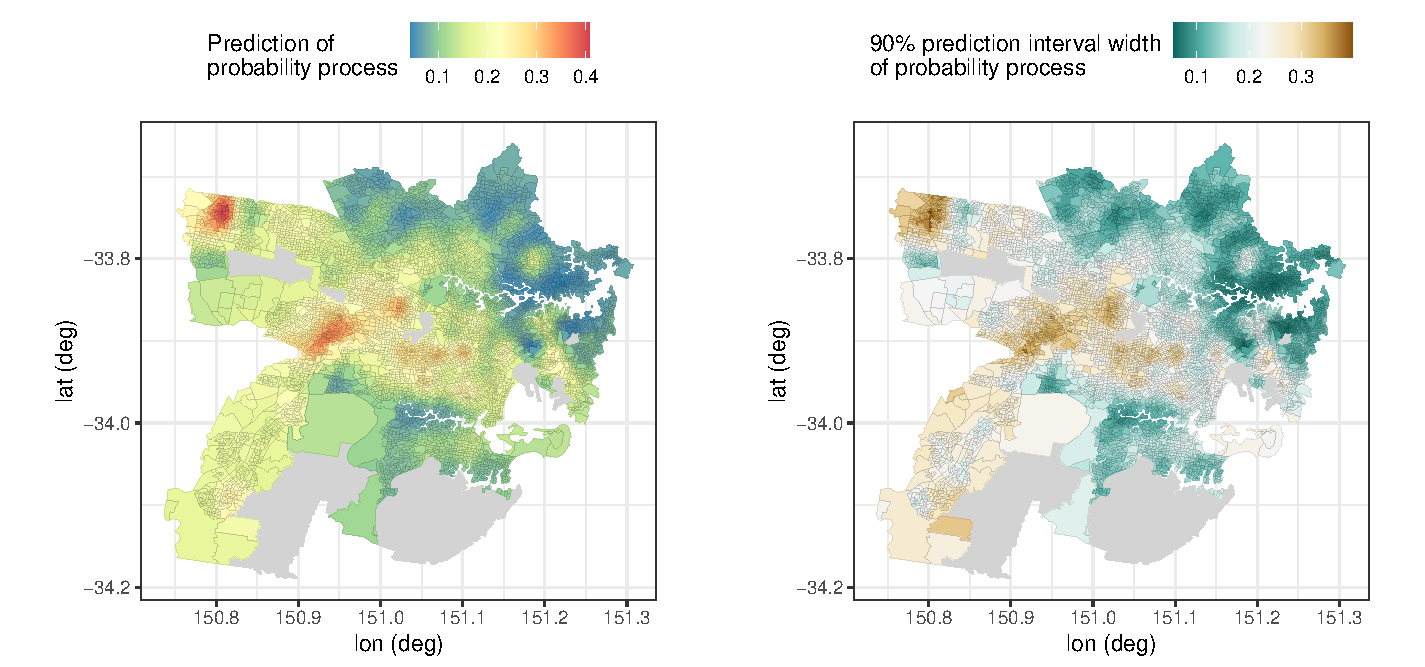
\includegraphics[width = \linewidth]{Images/Sydney_SA1_predictions.pdf}
    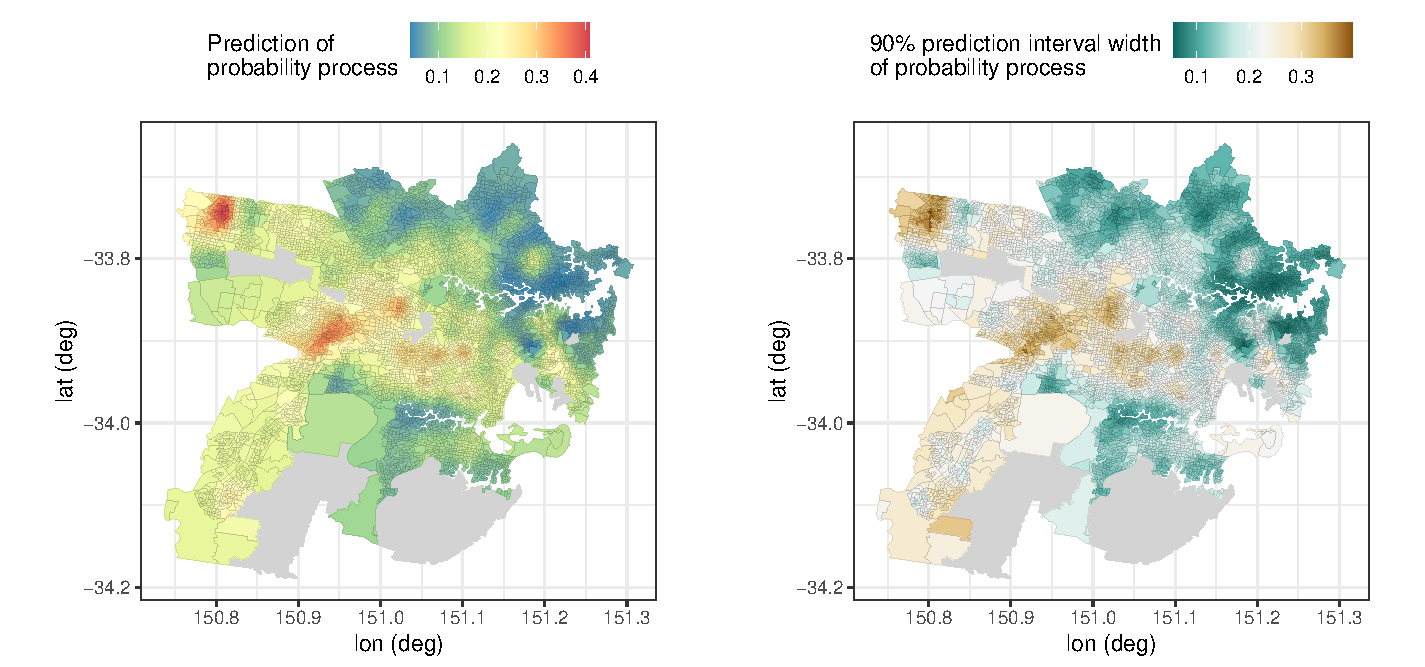
\includegraphics[width = \linewidth]{Images/Sydney_SA1_predictions.png}
    \caption{SA1 level predictions. (Left panel) Prediction of the probability process, $\pi(\cdot)$, representing the proportion of families in poverty, over the SA1 regions. (Right panel) 90\% prediction interval width of the probability process.
    Grey regions correspond to SA2 regions in which the total number of families is zero, and hence are omitted from the study. 
}   
  \label{fig:SA1_predictions}
\end{figure}



The first step of an analysis with \texttt{FRK} is to construct and fit the \texttt{SRE} object using the functions \texttt{SRE()} and \texttt{SRE.fit()}, or alternatively with the high-level and user-friendly wrapper \texttt{FRK()}. 
In this example, we provide the SA2 region data as training data, and the SA1 regions (no data included) as BAUs; these are passed as \texttt{SpatialPolygonDataFrame} objects to \texttt{FRK()}. 
We also set \texttt{normalise\_wts = FALSE}, which indicates that we wish to model the mean process in a given SA2 region as the sum of the mean process over the SA1s, rather than an average.
%\begin{minipage}{\linewidth}
%\begin{lstlisting}[style=R]
%S <- SRE(f = f, data = list(SA!2!s), basis = B, BAUs = SA!1!s, 
%         K_type = "neighbour", response = "binomial", link = "logit", 
%         normalise_wts = FALSE)
%\end{lstlisting}
%\end{minipage}
%As usual, the next step is to fit the \texttt{SRE} object with \texttt{SRE.fit()}.
Due to issues with identifiability, when the data support is areal with some supports comprising multiple BAUs,  \texttt{method = "TMB"} requires one to fix the fine-scale variance parameter, $\sigma^2_\xi$, before model fitting. 
In this situation, if $\sigma^2_\xi$ is unknown, \texttt{FRK} v.2 generates a rough estimate of it based on the initialisation procedure described in Appendix \ref{appendix:implementation_details}. 
If one does know $\sigma^2_\xi$, or can obtain a reliable estimate of it, they may specify it using the argument \texttt{known\_sigma2fs}.
%As we have SA1 data available, we are able to fit the model using the SA1 regions as both the BAUs \textit{and} the training data; %in this case
%%, although the data is areal, we do not need to fix the fine-scale variance parameter prior to model fitting, because every data support is associated with only a single BAU, and so 
% %we can estimate the fine-scale variance parameter using maximum likelihood estimation. 
%using this approach, we obtained a maximum likelihood estimate of $\hat{\sigma}^2_\xi = 0.2127$. 
%In practice SA1 data cannot be used if it is not available; one may use past census data, for example. 
%We tested prediction using both the rough and maximum likelihood estimates for $\sigma^2_\xi$, and discuss their effects on coverage later in this section. 

\begin{minipage}{\linewidth}
\begin{lstlisting}[style=R]
S <- FRK(f = total_poverty_count ~ 1, data = list(SA!2!s), BAUs = SA!1!s, 
         response = "binomial", link = "logit", 
         normalise_wts = FALSE)
\end{lstlisting}
\end{minipage}
         %, known_sigma!2!fs = 0.2127) 





%The call to fit the \texttt{SRE} object using the maximum likelihood estimate of the fine-scale variance is:


%\begin{minipage}{\linewidth}
%\begin{lstlisting}[style=R]
%S <- SRE.fit(S, method = "TMB", known_sigma!2!fs = 0.2127)
%\end{lstlisting}
%\end{minipage}

% The \texttt{known\_sigma2fs} argument allows us to fix the fine-scale variance prior to model fitting; this option is particularly useful in a spatial change-of-support setting, when one has a reliable estimate of the fine-scale variance from another source.
Generating predictions over different spatial supports is straightforward with \texttt{FRK} v.2.
First, we predict over the SA1 regions  (i.e., the BAUs) by calling \texttt{predict()}, and leaving the argument \texttt{newdata} as its default value of \texttt{NULL}:

\begin{minipage}{\linewidth}
\begin{lstlisting}[style=R]
SA!1!_predictions <- predict(S)
\end{lstlisting}
\end{minipage}

If we wish to predict over the SA3 regions, we simply set \texttt{newdata} to a  \texttt{SpatialPolygonDataFrame} object containing the SA3 regions:

\begin{minipage}{\linewidth}
\begin{lstlisting}[style=R]
SA!3!_predictions <- predict(S, newdata = SA!3!s)
\end{lstlisting}
\end{minipage}



As we use the SA1 regions as BAUs, we are able to generate predictions of both the probability and mean processes over the SA1 regions.
We focus on prediction of the probability process, which does not depend on the size parameter. 
The predictions, and associated uncertainty, of the probability process over the SA1 regions are displayed in Figure \ref{fig:SA1_predictions}.
As the SA3 regions are aggregations of the BAUs, we are only able to predict the mean process over the SA3 regions; Figure \ref{fig:SA3_predictions} displays the SA3 predictions and associated uncertainty quantification. 

\begin{figure}[t!]
    \centering
    \includegraphics[width = \linewidth]{Images/Sydney_SA3_predictions.pdf}
    \caption{SA3 level predictions. (Left panel) Prediction of the mean process, $\mu(\cdot)$, representing the expected number of families in poverty, over the SA3 regions. (Right panel) The 90\% prediction interval width of the mean process.
}   
  \label{fig:SA3_predictions}
\end{figure}




 We assessed the models ability quantify uncertainty over the SA1 regions by computing the empirical coverage from 90\% prediction intervals. 
 Using the rough estimate of $\sigma^2_\xi$, we observed an empirical coverage of 82.6\%, which indicates that, at least for this example, the rough estimate is reasonable. 
As we have SA1 data available, we are able to fit the model using the SA1 regions as both the BAUs \textit{and} the training data, which allows $\sigma^2_\xi$ to be estimated by maximum likelihood estimation; %in this case
%, although the data is areal, we do not need to fix the fine-scale variance parameter prior to model fitting, because every data support is associated with only a single BAU, and so 
 %we can estimate the fine-scale variance parameter using maximum likelihood estimation. 
 using this maximum likelihood estimate of $\sigma^2_\xi$ improved the coverage to 90.1\%, almost equal to the nominal coverage.
% In practice SA1 data cannot be used if it is not available; one may use past census data, for example. 
 Hence, if we have a way to obtain a reliable estimate of the fine-scale variance parameter (for example, using past census data), \texttt{FRK} v.2 can reliably quantify prediction uncertainty even in a spatial change-of-support setting. 
 

%% A naive predictor of the SA1 level proportion of families in poverty can be obtained by simply assigning the SA2 level proportions to its constituent SA1s. 
%A naive predictor of the proportion of families in poverty at the SA1 level can be obtained by simply computing the observed proportion of families in poverty for a given SA2 region, and then assigning this proportion the SA1 regions which comprise the given SA2 region.
%Such a naive predictor will result in an SA1 level prediction which is identical to the SA2 level training data displayed in the right panel of Figure \ref{fig:SA2_level_data}.
%In the absence of covariate information, predictive performance in spatial change-of-support problems is not necessarily improved by using \texttt{FRK} v.2 over a naive predictor. 
%% For instance, the resulting RMSPE when predicting the SA1 level data with \texttt{FRK} v.2 was 7.07, whilst the naive predictor scored 7.03.
%However, \texttt{FRK} v.2 can provide reliable uncertainty quantification (e.g., the width of predictive intervals), which is important, and difficult to obtain from a naive predictor.
%%Furthermore, the uncertainty quantification quantification provided by \texttt{FRK} v.2 is also reliable, as shown by the observed coverage of 90.1\% (when using the ``reliable'' estimate of the fine-scale variance) and 81.0\% (when using the ``rough'' estimate of the fine-scale variance) from purported 90\% prediction intervals. 
%\texttt{FRK} v.2 also allows covariate information to be considered, the inclusion of which would likely improve prediction over a naive predictor.






% \begin{figure}[t!]
%     \centering
%     \includegraphics[width = \linewidth]{Images/SA1_SA3_predictions.pdf}
%     \caption{SA2 level data. (Left panel) Observation and BAU supports. (Centre-left panel) True probability process at the BAU level. (Centre panel) Simulated data at the BAU level. (Centre-right panel) Aggregated data at the observation support level. (Right panel) Aggregated data with some observations missing.
% }   
%   \label{fig:SA1_SA3_predictions}
% \end{figure}









\subsection{Non-Gaussian spatio-temporal data: Crime in Chicago}\label{sec:ST_example}


The city of Chicago is divided into 77 so-called community areas. 
An attractive property of community areas is their relative consistency, their boundaries having changed little since their inception in the 1920's \citep{Chicago_library_census_data_info}. 
%Shapefiles for the community areas are available for download from the open data source website, Plenario (\url{http://plenar.io/explore/discover}), or directly from the city of Chicago website (\url{https://data.cityofchicago.org/}). 
Community area 76, which contains O'Hare airport, is almost disjoint from the other community areas, and is non-populous; for simplicity, we exclude this community area from this analysis.
In this study, we model the number of crimes in each community area between the years 2001 and 2019.
A full list of crimes committed in the city of Chicago during this period is provided by the Chicago Police Department, and is available for download from the open data source website Plenario \citep{Plenario_open_source_website}. 
%The full dataset has over 7 million crimes; however, here we consider only violent, non-sexual crimes, which we define as crimes labelled as assault or battery. 
We considered only violent, non-sexual crimes, which we defined as crimes labelled as assault or battery 
%(we excluded homicide, which is comparatively rare, with 10,324 recorded instances in our dataset).
(we excluded homicide, which is comparatively rare, accounting for less than 1\% of the violent crimes in our data). 
The data considered in this analysis consisted of 1,748,360 crimes.
% \red{(Noel and Andrew have suggested that we reference \cite{Rodrigues_2010_spatio-temporal_criminology}.)}


In this example, we use the community areas as our spatial BAUs. 
The community areas, a set of irregular polygons, can be used straightforwardly by reading in the shapefile of the community areas as a \texttt{SpatialPolygonsDataFrame} object. 
Spatio-temporal BAUs may then be constructed by passing the community areas and data into \texttt{auto\_BAUs()}.

\begin{minipage}{\linewidth}
\begin{lstlisting}[style=R]
## Construct spatio-temporal BAUs
ST_BAUs <- auto_BAUs(manifold = STplane(), data = chicago_crimes_fit,
                     spatial_BAUs = community_areas, tunit = "years")
ST_BAUs$fs <- 1 # scalar fine-scale covariance matrix
\end{lstlisting}
\end{minipage}

When modelling crimes, it is natural to include population, or population density, as a covariate. 
As the community areas are of unequal area, we use the raw population rather than population density.
%The U.S. Census Bureau does not compile data for community areas; to obtain population data at the community area level, 
We use 
the population data from the Combined Community Data Snapshots provided by the \cite{Chicago_community_data_snapshots}.
It is difficult to obtain population data for every year, so we assume the population is constant over the time-span of the data.
 We observed a distinct negative trend when plotting the total number of crimes in each year; hence, we also include time as a covariate.
%Figure \ref{fig:chicago_temporal_trend} shows the total number of crimes committed across Chicago in each year, and suggests that a piecewise, linear temporal model split by the year 2014 is appropriate. 
%The required BAU level covariates may be constructed in an analogous fashion to the way in which the covariates were constructed in Section \ref{sec:block_prediction}. 

%\begin{minipage}{\linewidth}
%\begin{lstlisting}[style=R]
%## Create population covariate
%ST_BAUs$population <- rep(community_areas$population, times = nt)
%
%## Covariates that can be used to make a piecewise temporal trend
%year <- ST_BAUs@data$t + 2000
%ST_BAUs$x!1! <- as.numeric(year < 2014)
%ST_BAUs$x!2! <- year * ST_BAUs$x!1!
%ST_BAUs$x!3! <- as.numeric(year >= 2014)
%ST_BAUs$x!4! <- year * ST_BAUs$x!3!
%\end{lstlisting}
%\end{minipage}


%Then, we automatically generate spatio-temporal basis functions by creating spatial basis functions with \texttt{auto\_basis()}, temporal basis functions with \texttt{local\_basis()}, and compute spatio-temporal basis functions by taking the tensor product of the spatial and temporal basis functions with \texttt{TensorP()}. 
Next, we generate spatio-temporal basis functions automatically with \texttt{auto\_basis()}.  
% Users who wish to have more control may construct the spatio-temporal basis functions manually by creating spatial basis functions with \texttt{auto\_basis()}, temporal basis functions with \mbox{\texttt{local\_basis()}}, and  computing the tensor product of the spatial and temporal basis functions with \texttt{TensorP()}.  
 
% Note that each observation in our dataset corresponds to an occurrence of a crime, and these crimes are indexed by the coordinates (longitude, latitude) and date at which the crime occurred; that is, we have unstructured spatio-temporal data in which observations may be recorded at any point in time and location in space. 
%Therefore, we store the full dataset, which we label as \mbox{\texttt{chicago\_crimes}}, as an object of class \texttt{STIDF}. 
%In a pre-processing step, we aggregated the number of crimes occurring at every unique coordinate and date combination, and stored this number as a field called \mbox{\texttt{number\_of\_crimes}}; the majority of entries in this field are 1, but it is possible that multiple crimes are recorded at the same location and time (for example, if there are multiple offenders, or if an offender is charged with multiple crimes in the same incident).
%A subset of the \mbox{\texttt{chicago\_crimes}} data, specifically, all of the data excluding the years 2010 and 2019, was used for training the model and automatically constructing the basis functions. %; this training subset is labelled \mbox{\texttt{chicago\_crimes\_fit}}.



\begin{minipage}{\linewidth}
\begin{lstlisting}[style=R]
## Spatio-temporal basis functions generated with a tensor product
basis <- auto_basis(STplane(), chicago_crimes_fit, tunit = "years")
\end{lstlisting}
\end{minipage}


%\begin{minipage}{\linewidth}
%\begin{lstlisting}[style=R]
%## Set up the spatial basis functions
%G_spatial <- auto_basis(manifold = plane(),         
%                        data = as(chicago_crimes_fit, "Spatial"))
%
%## Set up the temporal basis functions
%G_temporal <- local_basis(manifold = real_line(),     
%                          type = "Gaussian",          
%                          loc = matrix(seq(0, 20, length.out = 10)), 
%                          scale = rep(2,10))    
%
%## Spatio-temporal basis functions generated with a tensor product
%G <- TensorP(G_spatial, G_temporal) 
%\end{lstlisting}
%\end{minipage}


%Once the BAUs and basis functions are constructed, we use \texttt{SRE()} to initialise the \texttt{SRE} object, specifying \texttt{response = "poisson"} and \texttt{link = "log"}.
Once the BAUs and basis functions are constructed, we initialise and fit the \texttt{SRE} object using \texttt{FRK()}. 
 We have count data, so we set \texttt{response = "poisson"} and \texttt{link = "log"}.
 By default, \texttt{SRE()} averages observations falling into the same BAU. 
 If we wish to sum up instead of averaging, we pass the names of the variables to be summed to the argument \texttt{sum\_variables}; in this case, we want the total number of crimes occurring in each community area and each year, so we set \texttt{sum\_variables = "number\_of\_crimes"}.
As the number of spatial BAUs (the community areas) is relatively low, and we have observed each spatial BAU multiple times, we may attribute each spatial BAU its own fine-scale variance parameter (see Section \ref{sec:spatio-temporal}) by setting \texttt{fs\_by\_spatial\_BAU = TRUE}.

\begin{figure}[t!]
    \centering
    \includegraphics[width = \linewidth]{Images/chicago_validation_predictions.pdf}
    \caption{Observed and predicted number of crimes in the city of Chicago in the prediction (2010) and forecast (2019) years, as well as the associated prediction uncertainty. The first \textit{row} corresponds to the year 2010; the second row corresponds to the year 2019. The first \textit{column} displays the observed number of crimes; the second column displays the predicted number of crimes; the third column displays the 90\% posterior predictive interval width, which acts as a measure of uncertainty on the predictions.
}   
  \label{fig:chicago_validation_predictions}
\end{figure}

\begin{minipage}{\linewidth}
\begin{lstlisting}[style=R]
S <- FRK(f = number_of_crimes ~ log(population) + x!1! + x!2! + x!3!,   
         data = list(chicago_crimes_fit), basis = basis, BAUs = ST_BAUs,         
         response = "poisson", link = "log", 
         sum_variables = "number_of_crimes", fs_by_spatial_BAU = TRUE) 
\end{lstlisting}
\end{minipage}


Then, we predict over the BAUs (which have the community areas as spatial BAUs) using \texttt{predict()}, and plot the results using \texttt{plot()}.

%\begin{minipage}{\linewidth}
%\begin{lstlisting}[style=R]
%## Predict
%pred <- predict(S)
%
%## Plot
%subset_time <- c(2010, 2019) ## Years we wish to analyse
%plots <- plot(S, pred, binned_data, 
%              map_layer = chicago_map, subset_time = subset_time, 
%              colour = "black", size = 0.3, alpha = 0.85)
%
%## Change layout of each quantity to a single column, and edit axis
%plots <- lapply(plots, function(gg) gg + 
%                  facet_wrap(~t,  ncol = 1) + 
%                  xlab("lon (deg)") + ylab("lat (deg)"))
%                  
%## Arrange in a grid
%ggpubr::ggarrange(
%  plots$number_of_crimes, plots$p_Z, plots$interval_90_Z, 
%  align = "hv", nrow = 1, legend = "top"
%)
%
%\end{lstlisting}
%\end{minipage}

\begin{figure}[t!]
    \centering
    \includegraphics[width = \linewidth]{Images/chicago_time_series.pdf}
    \caption{Time-series plots of predictions and observed number of crimes for three community areas of interest. The validation years, 2010 and 2019, are highlighted in light-grey. The observed number of crimes at each time is indicated by a red point, whilst the predicted number of crimes is indicated by a blue point. The error bars represent a 90\% posterior predictive interval. We note that the posterior predictive intervals are slightly wider in validation years (2010 and 2019) than in observed years, and that the observed crime is contained within the predictive interval for all time-points for these community areas. 
}   
  \label{fig:chicago_time_series}
\end{figure}

\begin{figure}[t!]
    \centering
    \includegraphics[width = \linewidth]{Images/chicago_predictive_distributions.pdf}
    \caption{Posterior predictive distributions in the validation years (2010 and 2019) for three community areas (Archer Heights, Ashburn, and Roseland). The red and blue lines correspond to the observed and predicted number of crimes at each community area in the given year. 
    The first \textit{row} corresponds to the year 2010; the second row corresponds to the year 2019. The first \textit{column} corresponds to Archer Heights; the second column corresponds to Ashburn; the third column corresponds to Roseland. 
}   
  \label{fig:chicago_predictive_distributions}
\end{figure}


To validate predictions, we excluded the years 2010 and 2019 from the training data. 
The observed number of crimes, predicted number of crimes, and prediction uncertainty for these years are provided in Figure \ref{fig:chicago_validation_predictions}. 
Overall, for both years, Figure \ref{fig:chicago_validation_predictions} shows good agreement between the predicted and observed number of crimes. Furthermore, we can observe a distinct relationship between the prediction and the prediction uncertainty; specifically, the prediction uncertainty is roughly proportional to the predicted value, as one may expect when modelling counts.
For these validation years, we also computed the empirical coverage when using 90\%, 80\%, 70\%, and 60\% posterior predictive intervals, and the mean absolute percentage error (MAPE; see Appendix \ref{app:ScoringRules}). 
We consistently observed that the empirical coverage in the year 2010 was slightly (4\% on average) higher than the purported coverage, whilst it was lower (16\% on average) in the forecast year.
% For these validation years, we also computed the empirical coverage when using 90\%, posterior predictive intervals, and the mean absolute percentage error (MAPE; see Appendix \ref{app:ScoringRules}). 
% We empirical coverage in the year 2010 was slightly higher (94.7\%) than the purported coverage, whilst it was lower (76.3\%) in the forecast year. 
We observed MAPE scores of 4.4\% and 9.0\% in the years 2010 and 2019, respectively.
The slightly worse results in the year 2019 is possibly expected, as forecasting into the future is, in general, a harder task than predicting within the time-span of the data.
Nonetheless, these predictions are cause for optimism given the difficulties in modelling crime in a spatio-temporal setting. 


For illustration, we chose three community areas of interest; these community areas are Ashburn (community area 70), Roseland (community area 49), and Archer Heights (community area 57).
The time-series of the observed data, predictions, and 90\% posterior predictive intervals for these community areas is displayed in Figure \ref{fig:chicago_time_series}. 
We can see that the posterior predictive intervals are slightly wider in validation years (2010 and 2019) than in observed years, and that the observed crime is contained within the predictive interval for all time-points for these community areas.
The predictive distributions in the validation years for the three community areas of interest is given in Figure \ref{fig:chicago_predictive_distributions}.
The forecasts for Ashburn and Roseland in the year 2019 are particularly accurate, with the predicted number of crimes essentially equal to the observed number of crimes. 


% \begin{table}
%     \centering
%     \caption{Global results for the Chicago crime example.}
%     \label{tab:chicago_global_results}
%     \begin{tabular}{lccccc}
%     \hline\hline
%      Year  & MAPE & Cvg90 & Cvg80 & Cvg70 & Cvg60 \\[3pt]\hline
%     2010  & 4.38 & 94.7 & 85.5 & 73.7 & 67.1  \\
%     2019   & 8.51 & 77.6 & 67.1 & 53.9 & 46.1 \\
%     \hline
%   \end{tabular}
% \end{table}



\section{Conclusion}
\label{SEC:Conclusion}


In this paper we have described an extension to the \texttt{R} package \texttt{FRK} which allows for the spatial and spatio-temporal modelling and prediction of big, non-Gaussian data. 
Thanks to the use of a GLMM model and the software \texttt{TMB}, \texttt{FRK} v.2 can now cater for many distributions within the exponential family, and many link functions. 
Furthermore, \texttt{FRK} v.2 allows for the use of many more basis functions when modelling the spatial process, and can therefore also often achieve more accurate predictions in a Gaussian setting than \texttt{FRK} v.1. 
The existing functionality of \texttt{FRK} is retained with this extension; in particular, the package makes use of automatic basis function construction, is capable of handling both point-referenced and areal data, and eases the so-called spatial change-of-support problem through the use of BAUs.
The package now provides a highly accessible and user friendly approach to spatial and spatio-temporal modelling of big data in both a Gaussian and non-Gaussian setting.


One limitation of the framework is that it requires covariates to be known for every BAU, which may not be the case if covariates are recorded only at the data support level.
 Another limitation is the necessity to fix the fine-scale variance parameter in spatial change-of-support applications when \texttt{method = "TMB"}; note that this is not an issue if one is able to obtain a reliable estimate through other means (e.g., via previous census data). 
 \red{We are currently exploring avenues to address this limitation, either through adjusting the model to allow estimation of the fine-scale variance parameter within \texttt{TMB}, or via a more robust offline estimate.}
Another limitation is that despite the added flexibility, several models of interest, such as the zero-inflated Poisson, are still not catered for. 
 \red{The introduction of different types of models is facilitated by \texttt{TMB}s implementation of automatic differentiation, which means we can make use of existing code within the \texttt{C++} template straightforwardly; future work will see the introduction of other models of interest.}   
 \red{The main spatial data structures used in \texttt{FRK} come from the package \texttt{sp} \citep{Pebesma_2005_sp_package}; future work may entail the inclusion of other spatial data structures, such as those from the package \texttt{sf} \citep{Pebesma_2018_sf_package}.}
% Another is that, because of the separability of basis functions between space and time, the framework cannot capture interactions between space and time \citep[][Ch.~5]{Wikle_2019_ST_stats_with_R}. 
% (Mathematically, it can, but in practice, due to the compact support of the basis functions, the implied fields from the model are ''pseudo-stationary''.)
%\red{You also need to say that we are working on these limitations or something like that, and ideally also provide a sentence or two on how you envision to tackle them. They can be speculative.}


%\textbf{Acknowledgements}
%
%Dr.~Rajib Paul for his assistance with the Americium dataset.
%
%Data at the SA1, SA2, and SA3 levels used in the study of Section 4.2 were obtained from the
%Australian Bureau of Statistics web pages (Australian Bureau of Statistics, 2013, 2016, 2017).
%
%Dr.~Matt Moores for his discussion on the ethics of modelling crime in the city of Chicago. (Possibly add a brief discussion in the Chicago section on this topic, and reference the papers.) 
%
%Dr.~Michael Bertolacci for his discussion surrounding the MODIS comparison study, in particular, highlighting that the underlying distribution of $\pi(\cdot)$ is in fact unidentifiable, and that all of the moments of the predictive distribution of $\pi(\cdot)$ depend only on the posterior expectation, $\E{\pi(\cdot) \mid \vec{Z}}$.
%
%Need to cite \texttt{ggplot2} at some point.



%% References
\bibliographystyle{apalike}
% \bibliographystyle{references.bst}
% \cleardoublepage\phantomsection
\renewcommand{\bibname}{References}
\bibliography{FRKv2.bib}

%% Supp Material
%\renewcommand{\thefigure}{S\arabic{figure}}
%\setcounter{figure}{0}   
%\section{Supplementary material and figures}

%In this section we provide supplementary material and figures which were omitted from the main body for the sake of brevity. 

%Figure \ref{fig:BAU_intuition} is included to provide intuition on how BAUs are used within \texttt{FRK}.
%It shows how the continuous spatial domain $D$ is discretised into basic areal units (BAUs), the kind of supports permitted in \texttt{FRK} (both areal and point-referenced), and how the observation domain is constructed through observation supports. Figure \ref{fig:Poisson_multires} displays the prediction and prediction uncertainty when using a varying number of basis function resolutions, where the data used for model fitting is the point-referenced dataset shown in Figure \ref{fig:Poisson_true_and_Z}. Figure \ref{fig:chicago_temporal_trend} demonstrates that the period before 2014 exhibits a different temporal trend to the period after 2014 in terms of the number of crimes committed in Chicago. 




%\begin{figure}[t!]
%\centering
%\begin{tikzpicture}
%% Continuous domain D
%\begin{scope}[xshift = -4cm]
%\node at (1.5,4.5) {$D$};
%\draw (0, 0) rectangle (3, 4);% node [below left] {$D$};
%\end{scope}
%% Discretised domain, D^G
%\node at (1.5,4.5) {$D^G$};
%\draw[step=1cm] (0,0) grid (3,4);
%\node at (0.5,3.5) {$A_1$};
%\node at (1.5,3.5) {$A_2$};
%\node at (2.5,3.5) {$A_3$};
%\node at (0.5,2.5) {$A_4$};
%\node at (1.5,2.5) {$A_5$};
%\node at (2.5,2.5) {$A_6$};
%\node at (0.5,1.5) {$A_7$};
%\node at (1.5,1.5) {$A_8$};
%\node at (2.5,1.5) {$A_9$};
%\node at (0.5,0.5) {$A_{10}$};
%\node at (1.5,0.5) {$A_{11}$};
%\node at (2.5,0.5) {$A_{12}$};
%% Discretised domain, D_G, with observations
%\begin{scope}[xshift = 4cm]
%% \node at (1.5,4.5) {$D^O$};
%\draw[step=1cm] (0,0) grid (3,4);
%\filldraw[color=red, fill=red, opacity = 0.7] (0.25, 3.75) rectangle (1.1, 2.25);
%\filldraw[color=red, fill=red, opacity = 0.7] (0.15, 0.15) rectangle (1.85, 0.9);
%\filldraw[red, opacity = 0.7] (2.75,2.75) circle (0.08cm);
%\node at (0.5,3.5) {$A_1$};
%\node at (1.5,3.5) {$A_2$};
%\node at (2.5,3.5) {$A_3$};
%\node at (0.5,2.5) {$A_4$};
%\node at (1.5,2.5) {$A_5$};
%\node at (2.5,2.5) {$A_6$};
%\node at (0.5,1.5) {$A_7$};
%\node at (1.5,1.5) {$A_8$};
%\node at (2.5,1.5) {$A_9$};
%\node at (0.5,0.5) {$A_{10}$};
%\node at (1.5,0.5) {$A_{11}$};
%\node at (2.5,0.5) {$A_{12}$};
%\end{scope}
%% observation supports
%\begin{scope}[xshift = 8cm]
%\node at (1.5,4.5) {$D^O$};
%\draw[step=1cm] (0,4) grid (1,2);
%\draw[step=1cm] (0,0) grid (2,1);
%\draw[step=1cm] (2,2) grid (3,3);
%\node at (0.5,3.5) {$A_1$};
%\node at (0.5,2.5) {$A_4$};
%\node at (2.5,2.5) {$A_6$};
%\node at (0.5,0.5) {$A_{10}$};
%\node at (1.5,0.5) {$A_{11}$};
%
%\end{scope}
%\end{tikzpicture}
%\caption{A toy example demonstrating discretisation of the continuous spatial domain, and how the observation domain is derived from observations.
%(Left panel) The continuous spatial domain, $D$.
%(Centre-left panel) The discretised version of the spatial domain, $D^G$; in this example, $N = 12$ BAUs are used to tile the domain. 
%(Centre-right panel) The discretised domain after observing $m$ footprints; here, we have $m = 3$ footprints, two of which are areally referenced rectangles, while one is point referenced. 
%(Right panel) The observation domain, $D^O$; the observation supports which comprise $D^O$ are $B_1 = A_1 \cup A_4$,  $B_2 = A_6$, and $B_3 = A_{10} \cup A_{11}$.}\label{fig:BAU_intuition}
%\end{figure}




% Figure \ref{fig:02-04:TwoProbMass} is included to provide intuition on the maximum likelihood estimates obtained by maximising the marginal log-likelihood. 
% It shows two regions of probability mass in the joint distribution of the parameter and the random effects. 
% Although the left mass has a higher maximum joint likelihood in $L(\theta; u, \vec{Z})$, integrating out $u$ reveals that the right mass contributes more to the marginal likelihood $L(\theta; \vec{Z})$ than the left mass. Maximising $L(\theta; u, \vec{Z})$ would thus yield $\hat{\theta} = 0.5$; maximising $L^*(\theta; \vec{Z})$ (the Laplace approximation of $L(\theta; \vec{Z})$) on the other hand would yield $\hat{\theta} = 1.5$. Now, which estimate of $\vec{\theta}$ is preferred, the estimate derived from the joint likelihood function, or from the marginal likelihood function? If we were able to observe $\vec{u}$, then perhaps the estimate derived from the joint likelihood function would be preferable. However, if we are unable to observe $\vec{u}$, then it is wise to average over all possible values of $\vec{u}$; this leads to maximising the marginal likelihood. Since $\vec{u}$ is by definition unobserved, the estimate of $\vec{\theta}$ derived from $L(\vec{\theta}; \vec{Z})$ is preferred.


% \begin{figure}[t!]
%     \centering
%     \includegraphics[width = 0.75\linewidth]{Images/02-TwoProbMass.pdf}
%     \caption[Two regions of probability mass, demonstrating the different estimates of $\vec{\theta}$ which result from maximising the marginal and joint log-likelihood function]{Two regions of probability mass. The first, centred around $\theta = 0.5$, has a larger density than the second when $u$ is not marginalised out. However, the second, centred at $\theta = 1.5$, contributes more to the marginal likelihood $L(\theta; \vec{Z})$. Hence, an estimate of $\theta$ based on the marginal likelihood would yield $\hat{\theta} = 1.5$ and not $\hat{\theta} = 0.5$.}
%   \label{fig:02-04:TwoProbMass}
% \end{figure}



% \begin{figure}[t!]
%     \centering
%     \begin{subfigure}[b]{\linewidth}
%         \centering
%         \includegraphics[width=\linewidth]{Images/03-02-Poisson_plots2a.pdf}
%         \caption{(Left panel) True conditional mean of the data, $\muZgivenY{\cdot}$. (Right panel) Observed data.}\label{fig:03-02-PoissonResA}
%         \vspace{2\baselineskip}
%     \end{subfigure}
%     \begin{subfigure}[b]{\linewidth}
%         \centering
%         \includegraphics[width=\linewidth]{Images/03-02-Poisson_plots2b.pdf}
%         \caption{Prediction maps using basis functions of one resolution (left panel), two resolutions (centre panel), and three resolutions (right panel).}\label{fig:03-02-PoissonResB}
%         \vspace{2\baselineskip}
%     \end{subfigure}
%         \begin{subfigure}[b]{\linewidth}
%         \centering
%         \includegraphics[width=\linewidth]{Images/03-02-Poisson_plots2c.pdf}
%         \caption{Prediction uncertainty maps using basis functions of one resolution (left panel), two resolutions (centre panel), and three resolutions (right panel).}\label{fig:03-02-PoissonResC}
%         \vspace{2\baselineskip}
%     \end{subfigure}
%     \caption{\red{Use a common legend for each row if possible; probably use \texttt{facet\_wrap()} for the individual rows. We could reduce the size of the plot if we don't split into subfigures (i.e., have them as one big grid of plots). Perhaps we can omit this figure, or put it as an appendix.} Several panels summarising the analysis of a Poisson dataset using one, two, and three resolutions of basis functions. Clearly, detail of our predictions increases with an increasing number of resolutions used; this is apparent by comparing the smooth, relatively uniform prediction and uncertainty maps created using one resolution, to the more intricate maps generated using three resolutions. The prediction uncertainty also decreases as we use more basis functions.}
%     \label{fig:03-02-PoissonRes}
% \end{figure}



%\begin{figure}[t!]
%    \centering
%    \includegraphics[width = \linewidth]{Images/Poisson_multires.pdf}
%    \caption{Prediction and prediction uncertainty when analysing the Poisson data shown in Figure \ref{fig:Poisson_true_and_Z}. The first row corresponds to predictions of the mean process, $\mu(\cdot)$, while the second row corresponds to prediction uncertainty. The figure is divided into three columns, with the first, second, and third columns corresponding to predictions using one, two, and three resolutions of basis functions, respectively. 
%}   
%  \label{fig:Poisson_multires}
%\end{figure}


%\begin{figure}
%    \centering
%    \includegraphics[width = 0.7\linewidth]{Images/temporal_trend.pdf}
%    \caption{The total number of crimes committed across Chicago in each year, as well as two sets of fitted lines: the \red{red} line corresponds to a linear model that considers all data simultaneously, whilst the \textcolor{blue}{blue} line corresponds to a piecewise linear model split by the year 2014. The improved fit using a piecewise linear model suggests a piecewise temporal trend is appropriate for the Chicago analysis presented in Section \ref{sec:ST_example}.}   
%  \label{fig:chicago_temporal_trend}
%\end{figure}






%% Appendices
% \clearpage
\addtocontents{toc}{\protect\setcounter{tocdepth}{1}} % set only sections
\numberwithin{equation}{section}


\begin{appendices}
\section{Covariance tapering}
\label{Appendix:CovarianceTapering}

In this appendix, we provide details on the covariance tapering used to increase the sparsity of the prior variance matrix, $\vec{K}$, of the basis-function random coefficients. 
Note that, for computational reasons, when \texttt{method = "TMB"} we typically recommend setting \texttt{K\_type = "neighbour"}, which flags the use of a sparse prior precision matrix, $\vec{Q}$, for the basis-function random coefficients. 


Let $K_k(\vec{s}, \vec{s}^*)$ denote the covariance function of the random effects corresponding to the $k$th basis function resolution. 
 In \texttt{FRK}, we model $K_k(\vec{s}, \vec{s}^*)$ using the exponential covariance function,
\begin{equation}\label{eqn:02-01:K_covariance_function}
    K_k(\vec{s}, \vec{s}^*)  = \sigma^2_k \exp \left\{\frac{-d(\vec{s},\vec{s}^*)}{\tau_k}\right\}, 
\end{equation}
where $d(\vec{s},\vec{s}^*)$ is the distance between locations $\vec{s}, \vec{s}^* \in D$.  
 Given a covariance function we wish to taper, we must choose a taper function. 
 \citet{Furrer_2006_CovarianceTapering} recommend the Spherical taper for a Matérn covariance function with smoothness parameter $\nu\leq0.5$. 
 Noting that (\ref{eqn:02-01:K_covariance_function}) is special case of the Matérn covariance function with $\nu = 0.5$, we follow the recommendation of \cite{Furrer_2006_CovarianceTapering} and use the Spherical taper: 
\begin{equation}\label{eqn:02-01:taper_function}
K_{\beta_k}(\vec{s}, \vec{s}^*) 
=
\left\{1-\frac{d(\vec{s},\vec{s}^*)}{\beta_k}\right\}^2_{+}   \left\{1+\frac{d(\vec{s},\vec{s}^*)}{2\beta_k}\right\},
\end{equation}
where $x_{+} \equiv \max(0, x)$, and $\beta_k$ is a resolution-dependent tapering parameter controlling the strength of the taper. 
The taper is zero for $d(\vec{s},\vec{s}^*) \geq \beta_k$, and one for $d(\vec{s},\vec{s}^*) = 0$. 
The tapered covariance function for resolution $k$ is obtained by taking the product of the original covariance function (\ref{eqn:02-01:K_covariance_function}) and the taper function (\ref{eqn:02-01:taper_function}).%:
%\[
%{K_\textrm{tap}}_k(\vec{s}, \vec{s}^*)
% =
% K_k(\vec{s}, \vec{s}^*)K_{\beta_k}(\vec{s}, \vec{s}^*) 
%%=
%%\sigma^2_k \exp \left\{\frac{-d(\vec{s},\vec{s}^*)}{\tau_k}\right\}
%%\left\{1-\frac{d(\vec{s},\vec{s}^*)}{\beta_k}\right\}^2_{+}   \left\{1+\frac{d(\vec{s},\vec{s}^*)}{2\beta_k}\right\}
%,
%\]
%with the corresponding tapered variance-covariance matrix for resolution $k$ containing elements  
%\[
%    \{{\vec{K}_\textrm{tap}}_k\}_{i, j} 
%    = 
%    \sigma^2_k \exp \left\{\frac{-d(\vec{s}_{i, k},\vec{s}_{j, k})}{\tau_k}\right\}
%    \left\{1-\frac{d(\vec{s}_{i, k},\vec{s}_{j, k})}{\beta_k}\right\}^2_{+}   \left\{1+\frac{d(\vec{s}_{i, k},\vec{s}_{j, k})}{2\beta_k}\right\}.
%\]
%Finally, the full tapered variance-covariance matrix for the basis-function random effects $\vec{\eta}$ is thus
%\[
%\vec{K}_\textrm{tap} = 
%\begin{pmatrix}
%{\vec{K}_\textrm{tap}}_1   &           &           \\ 
%            & \ddots    &           \\
%            &           & {\vec{K}_\textrm{tap}}_l
%\end{pmatrix}.
%\]



To use this method of covariance-tapering we must specify the taper parameter $\beta_k$ for each resolution. 
% We first note that the basis functions created by \texttt{FRK} are constructed in a regular grid, whereby each resolution has $3^2=9$ times as many functions as the preceding resolution. 
% Hence, the effective range of three basis functions at resolution $k$ is equal to the effective range of a single basis function at resolution $k-1$. 
% We argue heuristically that basis functions at the $k$th resolution should not be used to capture scales that extend beyond a few ranges of the basis functions at the $(k-1)$th resolution. 
We do so based on the minimum distance between basis functions at the given resolution. Specifically, we set the tapering parameter of resolution $k$ to be $\beta_k = \texttt{taper} \times \text{mindist}(k)$, where $\text{mindist}(k)$ is the minimum distance between the centroids of basis functions at the $k$th resolution and \texttt{taper} is an argument set by the user which determines the strength of the covariance tapering. 
Decreasing $\beta_k$ will increase the sparsity of 
the tapered covariance matrix, %${\vec{K}_\textrm{tap}}_k$, 
 whilst increasing $\beta_k$ will decrease 
 %the sparsity of ${\vec{K}_\textrm{tap}}_k$.
 its sparsity.  
  Taking $\beta_k$ to infinity will recover the full block exponential covariance formulation.% of $\vec{K}_k$.

%Covariance tapering is done for computational reasons. In particular, the derivations and results in this work do not depend on whether the matrices $\vec{K}$ or $\vec{K}_\textrm{tap}$ are used. Hence, for notational convenience, we do not make a distinction between $\vec{K}$ and $\vec{K}_\textrm{tap}$.  




\section{Prediction}\label{app:prediction}

\numberwithin{equation}{subsection}

%\red{(I wonder if I can derive quantiles of the response distribution in the analytic case? I also wonder if it is possible to predict over arbitrary prediction regions in the analytic case (or, if it can only be done when we predict at the BAU level)? I think it would be informative to list all of the situations in which an analytic solution may be used, and when we must use MC sampling (using some kind of tree diagram). If it is only a very minor number of situations, then perhaps we can just omit the analytic approach.)}

In this appendix, we provide details for how we predict the latent process $Y(\cdot)$, the mean process $\mu(\cdot)$, and the noisy data process. 
%For simplicity, we provide details for the simple kriging case, whereby the fixed-effects $\vec{\alpha}$ are assumed to be known quantities, with the uncertainty of their estimation unaccounted for.
%The universal kriging case, which, in this framework, involves treating $\vec{\alpha}$ as random quantities, is a straightforward extension. 
For notational convenience, we treat the fixed effects and parameters, $\vec{\theta}$, as known.



\subsection{Prediction of the latent process $Y(\cdot)$}\label{sec:04-03-01:YProcessPrediction}


The predictor of $Y_i$, the latent process $Y(\cdot)$ evaluated over the BAU $A_i$, is the expectation of $Y_i$ conditional on the data, parameters, and fixed effects;
\begin{equation}\label{eqn:02-03:pYgivenZ}
    \pYgivenZ{A_i}
    \equiv
    \ECurly{Y_i \mid \vec{Z}, \vec{\theta}}.
\end{equation}
Recall from Section \ref{sec:marginal_likelihood} that the posterior distribution of the random effects, $\vec{u} \equiv (\vec{\eta}^\tp, \vec{\xi}^\tp)^\tp$, is approximated to be Gaussian (as we use the Laplace approximation), and hence the posterior distribution of $Y_i$ is also approximated to be Gaussian.
Therefore, another quantity of interest is the posterior variance;
\begin{equation}\label{eqn:02-03:varYgivenZ}
    \varCurly{Y_i \mid \vec{Z}, \vec{\theta}}.
\end{equation}
Given estimates of the posterior expectation and precision matrix of $\vec{u}$ using \texttt{TMB}, we are able to compute (\ref{eqn:02-03:pYgivenZ}) and (\ref{eqn:02-03:varYgivenZ}) in two ways. 
 The first is an analytic approach using basic expectation and variance properties, and the second is via Monte Carlo simulation.



\subsubsection{Analytic approach}

%Recall that for a location $\vec{s}\in D$, the process layer, irrespective of the assumed distribution of the data, is given by
%\[
%Y(\vec{s}) = \vec{t}(\vec{s})^\tp\vec{\alpha} + \phi(\vec{s})^\tp \vec{\eta} + \xi(\vec{s}); \quad \vec{s} \in D.
%\]
%Forms for the posterior expectation and variance can be derived straightforwardly. 
% However, before doing so, we explore a fact that will simplify some terms considerably. 

Recall that the process layer, irrespective of the assumed distribution of the data, is given by (\ref{eqn:04-01:Y(s)}). Defining $\vec{\xi}_O$ and $\vec{\xi}_U$ as the elements of $\vec{\xi}$ associated with observed and unobserved BAUs, respectively, it can be shown \citep[e.g.,][]{Sengupta_Cressie_2013_spatial_GLMM_FRK} that $\vec{\xi}_U$ are conditionally independent of all other random quantities in the model; that is, $[\vec{\xi}_U \mid \vec{Z}, \vec{\eta}, \vec{\xi}_O, \vec{\theta}] = [\vec{\xi}_U \mid \sigma^2_\xi]$. 
%Define $\vec{\xi}_O$ and $\vec{\xi}_U$ as the elements of $\vec{\xi}$ associated with observed and unobserved BAUs, respectively.
%\cite{Sengupta_Cressie_2013_spatial_GLMM_FRK} showed that, under the framework of a spatial GLMM with a spatial mixed effects model for the process layer, and assuming the fine-scale variation terms $\vec{\xi}$ are independent a priori, the unobserved fine-scale variation terms, $\vec{\xi}_U$, are conditionally independent of all other random quantities in the model; that is, that $[\vec{\xi}_U \mid \vec{Z}, \vec{\eta}, \vec{\xi}_O, \vec{\theta}] = [\vec{\xi}_U \mid \sigma^2_\xi]$.
%This allows for considerable simplification of the posterior expectation and variance at unobserved locations. 
%Specifically, (\ref{eqn:02-03:pYgivenZ}) becomes 
Then, the posterior expectation (\ref{eqn:02-03:pYgivenZ}) is 
\begin{align*}
    \pYgivenZ{A_i}
    &=
    \ECurly{Y_i \mid \vec{Z}, \vec{\theta}}\\
    &=
    \vec{t}(A_i)^\tp\vec{\alpha} + \vec{\phi}(A_i)^\tp \E{\vec{\eta} \mid \vec{Z}, \vec{\theta}} + \ECurly{\xi_i \mid \vec{Z}, \sigma^2_\xi}\\
    &=
    \begin{cases} 
      \vec{t}(A_i)^\tp\vec{\alpha} + \vec{\phi}(A_i)^\tp \E{\vec{\eta} \mid \vec{Z}, \vec{\theta}} + \ECurly{\xi_i \mid \vec{Z}, \sigma^2_\xi} & A_i\in D^O \\
      \vec{t}(A_i)^\tp\vec{\alpha} + \vec{\phi}(A_i)^\tp \E{\vec{\eta} \mid \vec{Z}, \vec{\theta}} & A_i\notin D^O
   \end{cases},
\end{align*}
where recall that $D^O$ denotes the set of observations supports. 
 The posterior variance (\ref{eqn:02-03:varYgivenZ}) is 
\begin{align*}
    &\varCurly{Y_i \mid \vec{Z}, \vec{\theta}} \nonumber \\
    &=
    \varCurly{\vec{\phi}(A_i)^\tp \vec{\eta} \mid \vec{Z}, \vec{\theta}}
    +
    \varCurly{\xi_i \mid \vec{Z}, \sigma^2_\xi}
    +
    2 \covCurlyConditional{ \vec{\phi}(A_i)^\tp\vec{\eta}}{\xi_i }{ \vec{Z}, \vec{\theta} } \nonumber \\
    &=
    \vec{\phi}(A_i)^\tp\vec{\Sigma}_{\vec{\eta} \mid \vec{Z}}\vec{\phi}(A_i)
    +
    \varCurly{\xi_i \mid \vec{Z}, \sigma^2_\xi}
    +
    2\vec{\phi}(A_i)^\tp
     \covCurlyConditional{ \vec{\eta} }{\xi_i }{\vec{Z}, \vec{\theta}} \nonumber \\
    &=
    \begin{cases}
    \vec{\phi}(A_i)^\tp\vec{\Sigma}_{\vec{\eta} \mid \vec{Z}}\vec{\phi}(A_i)
    +
    \varCurly{\xi_i \mid \vec{Z}, \sigma^2_\xi}
    +
    2\vec{\phi}(A_i)^\tp
    \covCurlyConditional{ \vec{\eta} }{ \xi_i }{ \vec{Z}, \vec{\theta} } & A_i\in D^O\\
    \vec{\phi}(A_i)^\tp\vec{\Sigma}_{\vec{\eta} \mid \vec{Z}}\vec{\phi}(A_i)
    +
    \sigma^2_\xi & A_i\notin D^O
    \end{cases},
\end{align*}
where $\vec{\Sigma}_{\vec{\eta} \mid \vec{Z}}$ is the posterior covariance matrix of the basis-function random coefficients.  
%Hence, for prediction and prediction uncertainty quantification of $Y_i$, we require the posterior expectation and variances of $\vec{\eta}$ and $\vec{\xi}_O$, as well as their posterior covariances. 
%Approximations of these values can be obtained using \texttt{TMB}. 
The posterior expectation of $\vec{u}$ is immediately available upon conclusion of model fitting.  
 However, \texttt{TMB} provides the posterior \textit{precision} matrix of $\vec{u}$, which must be inverted to obtain variances and covariances. 
The random effect block has dimension equal to the number of basis functions, $r$, plus the number of observed BAUs, $|D^O|$. 
Since $r + |D^O|$ is usually large, obtaining the covariance matrix of the random effects directly can be computationally prohibitive. 
We thus make use of the \textit{sparse-inverse-subset algorithm} (see \cite{Takahashi(1973)SparseInverseSubsetAlgorithm}; \cite{Rue_Martino_2007_Bayesian_inference_for_GMRF}; \cite{Zammit-Mangion_Rougier_2018_sparse_inverse_subset}) to obtain only the necessary elements of the covariance matrix; the sparse-inverse-subset algorithm is implemented with the \texttt{R} package \texttt{sparseinv} \citep{sparseinv_Package}. 
%This dramatically reduces the computational time to obtain the required posterior variances and covariances.


In practice, we do not perform a single calculation at a time; we use a matrix-vector form. In particular, the term $\vec{\phi}(A_i)^\tp   \vec{\Sigma}_{\vec{\eta} \mid \vec{Z}}   \vec{\phi}(A_i)$ can be computed for all locations via 
$$\diag{\vec{S} \vec{\Sigma}_{\vec{\eta} \mid \vec{Z}} \vec{S}^\tp} = \left(\vec{S} \vec{\Sigma}_{\vec{\eta}|\vec{Z}}\odot \vec{S}\right)\vec{1},$$
where $\odot$ denotes element-wise multiplication.


\subsubsection{Monte Carlo approach}

Rather than computing the expectation and variance of $Y_i$ analytically, we may instead generate Monte Carlo samples of $Y_i$, and then approximate the expectation and variance by the sample mean and sample variance, respectively. 
Monte Carlo simulation is required when inference is desired on the mean process or the noisy data (with some exceptions outlined in Section \ref{sec:prediction_mean_process}). 
%; namely, when the link function is the identity or log function, and when the data is Gaussian). %, and it may be useful if employing the sparse-inverse-subset algorithm is deemed to have a non-negligible effect on inference. 
Denote the posterior mode and precision matrix of the random effects by $\hat{\vec{u}}$ and $\vec{Q}_{u}$, respectively. 
Our approach involves simulating from the $\Gau(\hat{\vec{u}}, \vec{Q}_{u})$ distribution in order to generate Monte Carlo samples of $\vec{Y}$.
%
%Define a permuted version of the precision matrix as $\vec{A} \equiv \vec{P}^\tp \vec{Q}_{u} \vec{P}$, where $\vec{P}$ is a permutation matrix. Define the upper Cholesky factor of $\vec{A}$ as $\vec{U}_P$, which is the upper triangular matrix satisfying $\vec{A} = \vec{U}_P^\tp \vec{U}_P$. Then, we have that $\vec{Q}_{u} = \vec{M}^\tp \vec{M}$, where $\vec{M} = \vec{U}_P \vec{P}^\tp$ is \textit{not} triangular.
%Now consider the usual method of transforming a standard Gaussian vector to a Gaussian vector with precision matrix $\vec{Q}_{u}$. 
%First, let $\vec{z} \sim \Gau(\vec{0}, \vec{I})$ denote a standard Gaussian random vector. Then, we have that the variance of the transformed vector $\tilde{\vec{u}} \equiv \vec{M}^{-1}\vec{z} $ is
%\begin{align*}
%    \var{\tilde{\vec{u}}}
%    = \var{\vec{M}^{-1}\vec{z}}
%    = \vec{M}^{-1}\vec{M}^{-\tp}
%    = (\vec{M}^{\tp}\vec{M})^{-1}
%    = \vec{Q}_{u}^{-1},
%\end{align*}
%as required. Note, however, that although $\vec{M}$ is sparse, it is not triangular.
%However, we have that $\vec{M}^{-1} = \vec{P} \vec{U}_P^{-1}$,
%and so $\tilde{\vec{u}}$ may equivalently be written as
%$\tilde{\vec{u}} = \vec{P} \vec{U}_P^{-1}\vec{z}$.
%Therefore, we can first solve the upper triangular system $\vec{U}_P \vec{x} = \vec{z}$, and then left-multiply $\vec{x}$ by the permutation matrix $\vec{P}$ to obtain $\tilde{\vec{u}} = \vec{P} \vec{x} = \vec{P} \vec{U}_P^{-1}\vec{z} = \vec{M}^{-1}\vec{z}$, as required. 
%This approach to generating samples fully exploits both the reduction of fill-in from matrix reordering, as well as a computationally efficient backward-solve.
%
Once we have generated $n_{MC}$ samples of $\vec{u}$, we construct $\vec{Y}_{\text{MC}}$, an $N \times n_{MC}$ matrix whose $i$th row contains $n_{MC}$ Monte Carlo samples of $Y_i$, via 
\[
\vec{Y} 
= \vec{T}\vec{\alpha} + \vec{S}\vec{\eta} + \vec{\xi}
= \vec{T}\vec{\alpha} + 
%\begin{bmatrix}\vec{S} & \vec{I}\end{bmatrix} 
[\vec{S} \; \vec{I}]
\vec{u}
.
\]
Then, we may estimate (\ref{eqn:02-03:pYgivenZ}) and (\ref{eqn:02-03:varYgivenZ}) by taking row-wise means and variances of $\vec{Y}_{\text{MC}}$. 
%Further, samples from the mean process may be generated by passing the samples contained in $\vec{Y}^{MC}$ through the inverse-link function. 






\subsection{Prediction of the mean process}\label{sec:prediction_mean_process}


%Recall that the mean process, $\muZgivenY{\cdot}$, is modelled as a transformation of the latent process $Y(\cdot)$ via a link function $g(\cdot)$, so that $g\!\left(\muZgivenY{\cdot}\right) = Y(\cdot)$, or, equivalently,
%\begin{equation}\label{eqn:04-03:mu=psi(Y)}
%    \muZgivenY{\vec{s}} = g^{-1}\!\left(Y(\vec{s})\right), \quad \vec{s} \in D.
%\end{equation}
%Again, we use the posterior expectation as our predictor of (\ref{eqn:04-03:mu=psi(Y)}) at $A_i$;
Again, as predictor of $\mu_i$, the mean process $\mu(\cdot)$ evaluated the BAU $A_i$, we use the posterior expectation;
\begin{equation}\label{eqn:04-03:muOptimalPredictor}
    \pmugivenZ{A_i} 
    \equiv 
    \ECurly{\mu_i \mid \vec{Z}, \vec{\theta}}.
\end{equation}
% Again using the general result (\ref{eqn:04-03:GeneralMSPE}), the MSPE of (\ref{eqn:04-03:muOptimalPredictor}) when predicting the conditional mean $\muZgivenY{\cdot}$ at $A_i$ is 
% \begin{equation}\label{eqn:04-03:MSPEmuGivenZ1}
%     \MSPEtwoarg{\pmugivenZ{A_i}}{\muZgivenY{A_i}}
%     =
%     \ECurly{\var{\muZgivenY{A_i} \mid \vec{Z}}},
% \end{equation}
% which we again estimate by
% \begin{equation}\label{eqn:04-03:MSPEmuGivenZ2}
%     \MSPEtwoarg{\pmugivenZ{A_i}}{\muZgivenY{A_i}}
%     \approx
%     \varCurly{\muZgivenY{A_i} \mid \vec{Z}}
% \end{equation} 
% in the non-Gaussian case.
%Note that the assumptions made on the latent process $Y(\cdot)$ do not change, irrespective of the assumed response distribution and link function combination. 
%Hence, (\ref{eqn:02-03:pYgivenZ}) and (\ref{eqn:02-03:varYgivenZ}) remain as given in Section \ref{sec:04-03-01:YProcessPrediction} for all distributions and link functions supported by \texttt{FRK} v.2. 
Under certain link functions, (\ref{eqn:04-03:muOptimalPredictor}) may be evaluated analytically using (\ref{eqn:02-03:pYgivenZ}) and (\ref{eqn:02-03:varYgivenZ}). 
 This is trivially true for the identity link function.
Under the log-link function, as we approximate $Y_i \mid \vec{Z}, \vec{\theta}$ to be Gaussian, $g^{-1}\!\left(Y_i\right) \mid \vec{Z}, \vec{\theta}$ approximately follows a \textit{log-normal} distribution.
The expectation, variance, and quantile function (useful for uncertainty quantification) of a log-normal distribution are available in closed form. 
Specifically, under the log-link, the predictor (\ref{eqn:04-03:muOptimalPredictor}) is
\[
    \pmugivenZ{A_i}
    =
    \exp\left(\ECurly{Y_i \mid \vec{Z}, \vec{\theta}} + \frac{\varCurly{Y_i \mid \vec{Z}, \vec{\theta}}}{2}\right),
\]
the posterior variance is
\[
    \varCurly{\muZgivenY{A_i} \mid \vec{Z}, \vec{\theta}}
    =
    \left(e^{\varCurly{Y_i \mid \vec{Z}, \vec{\theta}}}-1\right)
    e^{2\ECurly{Y_i \mid \vec{Z}, \vec{\theta}}+\varCurly{Y_i \mid \vec{Z}, \vec{\theta}}},
\]
and the quantile function is
\[
Q(q)
=
\explr{
\ECurly{Y_i \mid \vec{Z}, \vec{\theta}} + \sqrt{2 \varCurly{Y_i \mid \vec{Z}, \vec{\theta}}}
\text{erf}^{-1}\!(2q - 1)
},
\]
where $\text{erf}^{-1}\!(\cdot)$ denotes the inverse error function.


When analytic solutions are not available, \texttt{FRK} v.2 employs Monte Carlo simulation. 
This is done by simulating samples of $Y_i$, and then transforming the samples via the mean function, $g^{-1}(\cdot)$. 
 In particular, we obtain Monte Carlo samples of $\vec{\mu}$, the mean process evaluated over the BAUs, via $g^{-1}(\vec{Y}_{\text{MC}})$. 
 Posterior expectations, variances, and quantiles may then be computed straightforwardly. 
 










\subsection{Prediction of the noisy data process}

We now turn our attention to prediction and prediction uncertainty of the noisy data process. 
Again, we use the posterior expectation as our predictor; 
\begin{equation}\label{eqn:04-03:ZOptimalPredictor}
    \hat{p}_{Z_i|\vec{Z}}
    \equiv 
    \ECurly{Z_i \mid \vec{Z}, \vec{\theta}}.
\end{equation}
Using the law of total expectation, 
% namely
% \[
% \E{A \mid B} = \ECurly{\E{A \mid B, C} \mid B}, 
% \]
we have that the predictor of $Z_i$ is
\begin{align*}
    \hat{p}_{Z_i|\vec{Z}}
    &=
    \ECurly{Z_i \mid \vec{Z}, \vec{\theta}}\\
    &=
    \ESquare{  \ECurly{Z_i \mid \vec{Z}, \vec{\theta}, \muZgivenY{A_i} }  \mid  \vec{Z}, \vec{\theta} }\\ 
    &=
    \ESquare{  \ECurly{Z_i \mid \muZgivenY{A_i}}  \mid  \vec{Z}, \vec{\theta} }\\
    &=
    \ESquare{  \muZgivenY{A_i}  \mid  \vec{Z}, \vec{\theta} }\\
    &=
    \pmugivenZ{A_i},
\end{align*}
and hence the predictor of $Z_i$ is equivalent to the predictor of the mean $\muZgivenY{A_i}$. 
% Again, for uncertainty quantification, we simply use prediction intervals obtained via Monte Carlo simulation.
The posterior variance $\varCurly{Z_i \mid \vec{Z}, \vec{\theta}}$ can be derived using the law of total conditional variance \citep[e.g.,][]{Bowsher_Swain_2012_total_conditional_variance}, 
% namely,
% \begin{equation}\label{eqn:04-03:LawOfTotalConditionalVariance} 
% \var{A \mid B} = \ECurly{\left.\var{A \mid B,C}\right|B} + \varCurly{\left.\E{A \mid B,C}\right|B},
% \end{equation}
so that
\begin{align}\label{eqn:var(Z|Z)}
    \varCurly{Z_i \mid \vec{Z}, \vec{\theta}}
    &=
    \ESquare{  \varCurly{  Z_i \mid \vec{Z}, \vec{\theta}, \mu_i    } \mid \vec{Z}, \vec{\theta}   } 
    + 
    \varSquare{  \ECurly{   Z_i \mid \vec{Z}, \vec{\theta}, \mu_i} \mid \vec{Z}, \vec{\theta}    }\nonumber\\
    &=
    \ESquare{   \varCurly{   Z_i \mid \mu_i   } \mid \vec{Z}, \vec{\theta}  } 
    + 
    \varSquare{ \ECurly{   Z_i \mid  \mu_i   } \mid \vec{Z}, \vec{\theta}}\nonumber\\
    &=
    \ESquare{   \varCurly{   Z_i \mid \mu_i   } \mid \vec{Z}, \vec{\theta}  } 
    + 
    \varCurly{ \muZgivenY{A_i} \mid \vec{Z}, \vec{\theta}}.
\end{align}
% This result makes intuitive sense. We have already shown that the predictors (\ref{eqn:04-03:muOptimalPredictor}) and (\ref{eqn:04-03:ZOptimalPredictor}) are equivalent, and so the difference in variance arises entirely from the differing variability of the predictands; a fact reflected by the term $\ESquare{   \varCurly{   Z_i \mid Y(A_i)   } \mid \vec{Z}  } $. Furthermore, it is well known that the uncertainty of an expectation is always lower than that of the corresponding data. 
Under certain distributions, this expression simplifies further. For instance, when the data is assumed to follow a Poisson distribution, (\ref{eqn:var(Z|Z)}) simplifies to 
\begin{align*}
 \varCurly{Z_i \mid \vec{Z}, \vec{\theta}}
&=
    \ECurly{\muZgivenY{A_i} \mid \vec{Z}, \vec{\theta}} 
    + 
    \varCurly{ \muZgivenY{A_i} \mid \vec{Z}, \vec{\theta}}\\
&=
\pmugivenZ{A_i}
    + 
    \varCurly{ \muZgivenY{A_i} \mid \vec{Z}, \vec{\theta}}.
\end{align*}
 When analytic solutions are not available, \texttt{FRK} v.2 again employs Monte Carlo simulation. 
  
 







% We now discuss details for prediction and uncertainty quantification for Gaussian and non-Gaussian data.

% \textit{Gaussian data}


% Although in the case of Gaussian data the focus of prediction is often on the process layer, we may also consider prediction on the data layer. The discussion above shows that the predictor of the noisy data process is equivalent to the predictor of the conditional mean of the data. However, this simplifies further in the case of Gaussian data. 
% Recall that for the Gaussian case $Z_i = Y(A_i)+\epsilon$, where $\epsilon$ represents independent measurement error with zero expectation. Thus (\ref{eqn:04-03:ZOptimalPredictor}) becomes
% \begin{align*}
%     \hat{p}_{Z_i|\vec{Z}}
%     &= 
%     \ECurly{Z_i \mid \vec{Z}}\\
%     &=
%     \ECurly{Y(A_i) \mid \vec{Z}} + \E{\epsilon \mid \vec{Z}}\\
%     &=
%     \ECurly{Y(A_i) \mid \vec{Z}}\\
%     &=
%     \pYgivenZ{A_i},
% \end{align*}
% and so we see that, in this case, prediction at the data layer is equivalent to prediction at the process layer. Again using the law of total conditional variance, the MSPE of (\ref{eqn:04-03:ZOptimalPredictor}) when the response is Gaussian is
% \begin{align*}
%     &\MSPEtwoarg{\hat{p}_{Z_i|\vec{Z}}}{Z_i}\\
%     &=
%     \ESquare{\varCurly{Z_i \mid \vec{Z}}}\\
%     &=
%     \varCurly{Z_i \mid \vec{Z}}\\
%     &=
%     \ESquare{  \varCurly{  Z_i \mid \vec{Z}, Y(A_i)    } \mid \vec{Z}   } 
%     + 
%     \varSquare{  \ECurly{   Z_i \mid \vec{Z}, Y(A_i)} \mid \vec{Z}}\\
%     &=
%     \ESquare{   \varCurly{   Z_i \mid Y(A_i)   } \mid \vec{Z}} 
%     + 
%     \varSquare{ \ECurly{   Z_i \mid  Y(A_i)   } \mid \vec{Z}}\\
%     &=
%     \E{\sigma^2_\epsilon \mid \vec{Z}} 
%     + 
%     \varCurly{Y(A_i) \mid \vec{Z}}\\
%     &=
%     \sigma^2_\epsilon +
%     \varCurly{Y(A_i) \mid \vec{Z}}\\
%     &=
%     \sigma^2_\epsilon + 
%     \MSPEtwoarg{\pYgivenZ{A_i}}{Y(A_i)}.
% \end{align*}
% This is intuitively reasonable; the additional uncertainty in our prediction of the data layer arises from the fact that $Z(\cdot)$ is a noisy version of $Y(\cdot)$, with noise coming from independent measurement error.


% \textit{Non-Gaussian data}


% In a non-Gaussian setting, prediction and prediction uncertainty is more often focused on the noisy data process $Z(\cdot)$; in these situations, we are interested in the predictor (\ref{eqn:04-03:ZOptimalPredictor}) and its associated mean square prediction error. We have proven that, in all cases, irrespective of the distribution of the response variable, (\ref{eqn:04-03:ZOptimalPredictor}) is equivalent to (\ref{eqn:04-03:muOptimalPredictor}), the predictor of the conditional mean of the data. Furthermore, we have shown that, in general, 
% \[
% \MSPEtwoarg{\hat{p}_{Z_i|\vec{Z}}}{Z_i}
% \approx
%     \ECurly{   \varCurly{ Z_i \mid Y(A_i) } \mid \vec{Z}  } 
%     + 
%     \MSPEtwoarg{\pmugivenZ{A_i}}{\muZgivenY{A_i}}.
% \]
% As variance is, by definition, a positive quantity, the prediction variance on the $Z$-scale is always greater than the variance for the expectation $\muZgivenY{\cdot}$, which is reasonable as $Z(\cdot)$ is a noisy process. 
% Under some distributions, this expression simplifies further. For instance, when the data has a Poisson distribution, this simplifies to 
% \begin{align*}
% \MSPEtwoarg{\hat{p}_{Z_i|\vec{Z}}}{Z_i}
% &\approx
%     \ECurly{\muZgivenY{A_i} \mid \vec{Z}} 
%     + 
%     \MSPEtwoarg{\pmugivenZ{A_i}}{\muZgivenY{A_i}}\\
% &=
% \pmugivenZ{A_i}
%     + 
%     \MSPEtwoarg{\pmugivenZ{A_i}}{\muZgivenY{A_i}}.
% \end{align*}


















% \subsection{Prediction of the conditional mean of the data}


% Recall that the response variable is assumed to follow a distribution from the exponential-family, with conditional mean $\muZgivenY{\cdot}$ modelled as a transformation of the latent process $Y(\cdot)$ by a link function $g(\cdot)$, so that $g\!\left(\muZgivenY{\vec{s}}\right) = Y(\vec{s})$, or, equivalently,
% \begin{equation}\label{eqn:04-03:mu=psi(Y)}
%     \muZgivenY{\vec{s}} = g^{-1}\!\left(Y(\vec{s})\right), \quad \vec{s} \in D.
% \end{equation}
% The best (again in terms of mean-squared prediction error) predictor of (\ref{eqn:04-03:mu=psi(Y)}) at $\vec{s}_0$ is 
% \begin{equation}\label{eqn:04-03:muOptimalPredictor}
%     \pmugivenZ{\vec{s}_0} 
%     \equiv 
%     \ECurly{g^{-1}\!\left(Y(\vec{s}_0)\right) \mid \vec{Z}}.
% \end{equation}
% Again using the general result (\ref{eqn:04-03:GeneralMSPE}), the MSPE of (\ref{eqn:04-03:muOptimalPredictor}) when predicting the conditional mean $\muZgivenY{\cdot}$ at $\vec{s}_0$ is 
% \begin{equation}\label{eqn:04-03:MSPEmuGivenZ1}
%     \MSPEtwoarg{\pmugivenZ{\vec{s}_0}}{\muZgivenY{\vec{s}_0}}
%     =
%     \ECurly{\var{\muZgivenY{\vec{s}_0} \mid \vec{Z}}},
% \end{equation}
% which we again estimate by
% \begin{equation}\label{eqn:04-03:MSPEmuGivenZ2}
%     \MSPEtwoarg{\pmugivenZ{\vec{s}_0}}{\muZgivenY{\vec{s}_0}}
%     \approx
%     \varCurly{\muZgivenY{\vec{s}_0} \mid \vec{Z}}
% \end{equation} 
% in the non-Gaussian case.

% The details regarding prediction of the conditional mean $\muZgivenY{\cdot}$ depend on the chosen link function $g(\cdot)$.  When an identity link-function is used, or when a log-link function is used, (\ref{eqn:04-03:muOptimalPredictor}) and (\ref{eqn:04-03:MSPEmuGivenZ2}) may be evaluated exactly. However, in general this is not possible. In these instances, we must approximate (\ref{eqn:04-03:muOptimalPredictor}) and (\ref{eqn:04-03:MSPEmuGivenZ2}) analytically (using a Taylor series expansion, for example) or via Monte Carlo simulation. In \texttt{FRK} we choose to use Monte Carlo simulation. 

% Note that the assumptions we made on the latent spatial process $Y(\cdot)$ do not change, irrespective of the assumed response distribution and link function combination. Hence, prediction and uncertainty quantification on the $Y$-scale, $\pYgivenZ{\vec{s}_0}$ and  $\MSPEtwoarg{\pYgivenZ{\vec{s}_0}}{Y(\vec{s}_0)}$, remain as given in Section \ref{sec:04-03-01:YProcessPrediction}, for any distribution and link function. 


% \textit{Identity link function}


% When the link function is the identity function (which is typically the case for a Gaussian response variable), prediction of the conditional mean is equivalent to prediction of the $Y(\cdot)$ process. Hence, the predictor $\pmugivenZ{\vec{s}_0}$ is equivalent to $\pYgivenZ{\vec{s}_0}$, and the prediction uncertainty $\MSPEtwoarg{\pmugivenZ{\vec{s}_0}}{\muZgivenY{\vec{s}_0}}$ is equivalent to $\MSPEtwoarg{\pYgivenZ{\vec{s}_0}}{Y(\vec{s}_0)}$; these quantities remain as given in Section \ref{sec:04-03-01:YProcessPrediction}.  



% \textit{Log-link function}

% As $Y(\vec{s}_0) \mid \vec{Z}$ is Gaussian, when we assume a log-link function,  $\muZgivenY{\vec{s}_0} | \vec{Z} \equiv \exp\left\{Y(\vec{s}_0)\right\} | \vec{Z}$ follows a \textit{log-normal} distribution. Conveniently, the expectation and variance of a log-normal distribution have analytic forms, and so we may evaluate the predictor (\ref{eqn:04-03:muOptimalPredictor}) and its associated mean-squared prediction error (\ref{eqn:04-03:MSPEmuGivenZ2}) exactly. Specifically, (\ref{eqn:04-03:muOptimalPredictor}) is given by
% \begin{align*}
%     \pmugivenZ{\vec{s}_0}
%     &=
%     \ECurly{\muZgivenY{\vec{s}_0} \mid \vec{Z}} \\
%     &=
%     \ECurly{\exp\left\{Y(\vec{s}_0)\right\} \mid \vec{Z}}\\
%     &=
%     \exp\left(\ECurly{Y(\vec{s}_0) \mid \vec{Z}} + \frac{\varCurly{Y(\vec{s}_0) \mid \vec{Z}}}{2}\right)\\
%     &\approx
%     \exp\left(\pYgivenZ{\vec{s}_0} + \frac{\MSPEtwoarg{\pYgivenZ{\vec{s}_0}}{Y(\vec{s}_0)}}{2}\right),
% \end{align*}
% and the mean-squared prediction error (\ref{eqn:04-03:MSPEmuGivenZ2}) is
% \begin{align*}
%     &\MSPEtwoarg{\pmugivenZ{\vec{s}_0}}{\muZgivenY{\vec{s}_0}}\\
%     &\approx
%     \varCurly{\muZgivenY{\vec{s}_0} \mid \vec{Z}}\\
%     &=
%     \left(\exp\left\{\varCurly{Y(\vec{s}_0) \mid \vec{Z}}\right\}-1\right)
%     \exp\left\{2\ECurly{Y(\vec{s}_0) \mid \vec{Z}}+\varCurly{Y(\vec{s}_0) \mid \vec{Z}}\right\}\\
%     &\approx
%     \left(\exp\left\{\MSPEtwoarg{\pYgivenZ{\vec{s}_0}}{Y(\vec{s}_0)}\right\}-1\right)
%     \exp\left\{2\pYgivenZ{\vec{s}_0}+\MSPEtwoarg{\pYgivenZ{\vec{s}_0}}{Y(\vec{s}_0)}\right\}.
% \end{align*}








% \textit{Other Link Functions}

% Most of the frequently used link functions do not share the desirable analytic properties of the log-link function. Take, for example, the logit-link function (which is canonical for Bernoulli data). The conditional mean $\muZgivenY{\cdot}$ under the logit-link function has a \textit{Logit-normal} distribution. Unfortunately, the expectation and variance (indeed all moments) of a Logit-normal distribution have no analytic solution. Hence, in this case we are unable to compute the predictor (\ref{eqn:04-03:muOptimalPredictor}) or its mean-squared prediction error (\ref{eqn:04-03:MSPEmuGivenZ2}) exactly. Instead, we approximate their value via Monte Carlo sampling. 



% \subsection{Prediction of the noisy data process}

% We now turn our attention to prediction and prediction uncertainty of the noisy data process $Z(\cdot)$. In some cases (particularly for non-Gaussian data) we seek prediction not on the smooth spatial processes $Y(\cdot)$ and $\muZgivenY{\cdot}$, but on the noisy data process $Z(\cdot)$. In this case, the predictor we choose is 
% \begin{equation}\label{eqn:04-03:ZOptimalPredictor}
%     \pZgivenZ{\vec{s}_0} 
%     \equiv 
%     \ECurly{Z(\vec{s}_0) \mid \vec{Z}}.
% \end{equation}
% Using a general form of the law of total expectation, namely
% \[
% \E{A \mid B} = \ECurly{\E{A \mid B, C} \mid B}, 
% \]
% we have that the prediction on the $Z$-scale is given by
% \begin{align*}
%     \pZgivenZ{\vec{s}_0}
%     &=
%     \ECurly{Z(\vec{s}_0) \mid \vec{Z}}\\
%     &=
%     \ESquare{  \ECurly{Z(\vec{s}_0) \mid \vec{Z}, Y(\vec{s}_0)}  \mid  \vec{Z} }\\ 
%     &=
%     \ESquare{  \ECurly{Z(\vec{s}_0) \mid Y(\vec{s}_0)}  \mid  \vec{Z} }\\
%     &=
%     \ESquare{  \muZgivenY{\vec{s}_0}  \mid  \vec{Z} }\\
%     &=
%     \pmugivenZ{\vec{s}_0},
% \end{align*}
% and hence the predictor of the data process is equivalent to the predictor of the conditional mean $\muZgivenY{\cdot}$. However, the mean-squared prediction error depends on both the predictor \textit{and} the predictand. For this reason, despite the fact that (\ref{eqn:04-03:muOptimalPredictor})  and (\ref{eqn:04-03:ZOptimalPredictor}) are equivalent predictors, we will retain the notational distinction, as the MSPE's associated with each predictor are different.
% The MSPE of (\ref{eqn:04-03:ZOptimalPredictor}) when predicting the data process $Z(\cdot)$ at $\vec{s}_0$ can be derived using the law of total conditional variance \citep{Bowsher_Swain_2012_total_conditional_variance}, namely,
% \begin{equation}\label{eqn:04-03:LawOfTotalConditionalVariance}
% \var{A \mid B} = \ECurly{\left.\var{A \mid B,C}\right|B} + \varCurly{\left.\E{A \mid B,C}\right|B}.
% \end{equation}
% The MSPE of (\ref{eqn:04-03:ZOptimalPredictor}) when predicting $Z(\cdot)$ at $\vec{s}_0$ is then
% \begin{align*}
%     &\MSPEtwoarg{\pZgivenZ{\vec{s}_0}}{Z(\vec{s}_0)}\\
%     &=
%     \E{\varCurly{Z(\vec{s}_0) \mid \vec{Z}}}\\
%     &\approx
%     \varCurly{Z(\vec{s}_0) \mid \vec{Z}}\\
%     &=
%     \ESquare{  \varCurly{  Z(\vec{s}_0) \mid \vec{Z}, Y(\vec{s}_0)    } \mid \vec{Z}   } 
%     + 
%     \varSquare{  \ECurly{   Z(\vec{s}_0) \mid \vec{Z}, Y(\vec{s}_0)} \mid \vec{Z}    }\\
%     &=
%     \ESquare{   \varCurly{   Z(\vec{s}_0) \mid Y(\vec{s}_0)   } \mid \vec{Z}  } 
%     + 
%     \varSquare{ \ECurly{   Z(\vec{s}_0) \mid  Y(\vec{s}_0)   } \mid \vec{Z}}\\
%     &=
%     \ESquare{   \varCurly{   Z(\vec{s}_0) \mid Y(\vec{s}_0)   } \mid \vec{Z}  } 
%     + 
%     \varCurly{ \muZgivenY{\vec{s}_0} \mid \vec{Z}}\\
%     &\approx
%     \ESquare{   \varCurly{   Z(\vec{s}_0) \mid Y(\vec{s}_0)   } \mid \vec{Z}  }  
%     + 
%     \MSPEtwoarg{\pmugivenZ{\vec{s}_0}}{\muZgivenY{\vec{s}_0}},
% \end{align*}
% where the first approximate equality is in fact an equality in the case of Gaussian data, and the last line is the estimation (\ref{eqn:04-03:MSPEmuGivenZ2}), which again is an equality in the case of Gaussian data. This result makes intuitive sense. We have already shown that the predictors (\ref{eqn:04-03:muOptimalPredictor}) and (\ref{eqn:04-03:ZOptimalPredictor}) are equivalent, and so the difference in MSPE arises entirely from the differing variability of the predictands; a fact reflected by the term $\ESquare{   \varCurly{   Z(\vec{s}_0) \mid Y(\vec{s}_0)   } \mid \vec{Z}  } $. Furthermore, it is well known that the uncertainty of an expectation is always lower than that of the corresponding data. 

% We now discuss details for prediction and uncertainty quantification for Gaussian and non-Gaussian data.

% \textit{Gaussian data}


% Although in the case of Gaussian data the focus of prediction is often on the process layer, we may also consider prediction on the data layer. The discussion above shows that the predictor of the noisy data process is equivalent to the predictor of the conditional mean of the data. However, this simplifies further in the case of Gaussian data. 
% Recall that for the Gaussian case $Z(\vec{s}_0) = Y(\vec{s}_0)+\epsilon$, where $\epsilon$ represents independent measurement error with zero expectation. Thus (\ref{eqn:04-03:ZOptimalPredictor}) becomes
% \begin{align*}
%     \pZgivenZ{\vec{s}_0}
%     &= 
%     \ECurly{Z(\vec{s}_0) \mid \vec{Z}}\\
%     &=
%     \ECurly{Y(\vec{s}_0) \mid \vec{Z}} + \E{\epsilon \mid \vec{Z}}\\
%     &=
%     \ECurly{Y(\vec{s}_0) \mid \vec{Z}}\\
%     &=
%     \pYgivenZ{\vec{s}_0},
% \end{align*}
% and so we see that, in this case, prediction at the data layer is equivalent to prediction at the process layer. Again using the law of total conditional variance, the MSPE of (\ref{eqn:04-03:ZOptimalPredictor}) when the response is Gaussian is
% \begin{align*}
%     &\MSPEtwoarg{\pZgivenZ{\vec{s}_0}}{Z(\vec{s}_0)}\\
%     &=
%     \ESquare{\varCurly{Z(\vec{s}_0) \mid \vec{Z}}}\\
%     &=
%     \varCurly{Z(\vec{s}_0) \mid \vec{Z}}\\
%     &=
%     \ESquare{  \varCurly{  Z(\vec{s}_0) \mid \vec{Z}, Y(\vec{s}_0)    } \mid \vec{Z}   } 
%     + 
%     \varSquare{  \ECurly{   Z(\vec{s}_0) \mid \vec{Z}, Y(\vec{s}_0)} \mid \vec{Z}}\\
%     &=
%     \ESquare{   \varCurly{   Z(\vec{s}_0) \mid Y(\vec{s}_0)   } \mid \vec{Z}} 
%     + 
%     \varSquare{ \ECurly{   Z(\vec{s}_0) \mid  Y(\vec{s}_0)   } \mid \vec{Z}}\\
%     &=
%     \E{\sigma^2_\epsilon \mid \vec{Z}} 
%     + 
%     \varCurly{Y(\vec{s}_0) \mid \vec{Z}}\\
%     &=
%     \sigma^2_\epsilon +
%     \varCurly{Y(\vec{s}_0) \mid \vec{Z}}\\
%     &=
%     \sigma^2_\epsilon + 
%     \MSPEtwoarg{\pYgivenZ{\vec{s}_0}}{Y(\vec{s}_0)}.
% \end{align*}
% This is intuitively reasonable; the additional uncertainty in our prediction of the data layer arises from the fact that $Z(\cdot)$ is a noisy version of $Y(\cdot)$, with noise coming from independent measurement error.


% \textit{Non-Gaussian data}


% In a non-Gaussian setting, prediction and prediction uncertainty is more often focused on the noisy data process $Z(\cdot)$; in these situations, we are interested in the predictor (\ref{eqn:04-03:ZOptimalPredictor}) and its associated mean square prediction error. We have proven that, in all cases, irrespective of the distribution of the response variable, (\ref{eqn:04-03:ZOptimalPredictor}) is equivalent to (\ref{eqn:04-03:muOptimalPredictor}), the predictor of the conditional mean of the data. Furthermore, we have shown that, in general, 
% \[
% \MSPEtwoarg{\pZgivenZ{\vec{s}_0}}{Z(\vec{s}_0)}
% \approx
%     \ECurly{   \varCurly{ Z(\vec{s}_0) \mid Y(\vec{s}_0) } \mid \vec{Z}  } 
%     + 
%     \MSPEtwoarg{\pmugivenZ{\vec{s}_0}}{\muZgivenY{\vec{s}_0}}.
% \]
% As variance is, by definition, a positive quantity, the prediction variance on the $Z$-scale is always greater than the variance for the expectation $\muZgivenY{\cdot}$, which is reasonable as $Z(\cdot)$ is a noisy process. 
% Under some distributions, this expression simplifies further. For instance, when the data has a Poisson distribution, this simplifies to 
% \begin{align*}
% \MSPEtwoarg{\pZgivenZ{\vec{s}_0}}{Z(\vec{s}_0)}
% &\approx
%     \ECurly{\muZgivenY{\vec{s}_0} \mid \vec{Z}} 
%     + 
%     \MSPEtwoarg{\pmugivenZ{\vec{s}_0}}{\muZgivenY{\vec{s}_0}}\\
% &=
% \pmugivenZ{\vec{s}_0}
%     + 
%     \MSPEtwoarg{\pmugivenZ{\vec{s}_0}}{\muZgivenY{\vec{s}_0}}.
% \end{align*}


\section{Distributions with size parameters}\label{sec:Distributions with size parameters}

Two data models that can be used with \texttt{FRK} v.2, namely, the binomial and negative-binomial distributions, have a known constant ``size'' parameter $k_j$ and a ``probability of success'' parameter, $\pi_j$, associated with every datum $Z_j$.
For binomial data models, $k_j$ represents the number of trials, and $Z_j$ the number of successes; for negative-binomial data models, $k_j$ represents the target number of successes, and $Z_j$ the number of failures. 

Consider a negative-binomial data model with a logit-link function; under the standard interpretation of a link function (a function which transforms the mean $\mu(\cdot)$ to the linear predictor $Y(\cdot)$), one models 
\[
g(\mu(\cdot)) = \logit{\mu(\cdot)} = Y(\cdot).
\]
In this example, the range of the mean function (the inverse link function, $g^{-1}(\cdot)$) is $(0, 1)$.
However, the mean of negative-binomial distribution may take values in $[0, \infty)$. 
Direct use of the logit link would thus unacceptably restrict the range of the mean function.

Therefore, for both the binomial and negative-binomial distributions, we first model $\pi(\cdot)$ as a function of $Y(\cdot)$, and then link $\pi(\cdot)$ to the mean $\muZgivenY{\cdot}$. 
That is, we use a hierarchical link function;
\begin{gather*}
    f(\pi(\cdot)) = Y(\cdot),\\
    h(\mu(\cdot); k) = \pi(\cdot), 
\end{gather*}
where $h(\cdot)$ is a function determined solely by the response distribution, and $f(\cdot)$ is a function that maps $\pi(\cdot)$ to the latent process $Y(\cdot)$.  
The implied link function is
\[
g(\mu(\cdot); k) = f(h(\mu(\cdot); k)) = (f \circ h)(\mu(\cdot); k) = Y(\cdot).
\]
Using a hierarchical link function approach with a negative-binomial data model and a logit-link function, we have that
\[
f(\pi(\cdot)) = \logit{\pi(\cdot)} = Y(\cdot),
\]
and, as the expectation of the negative-binomial distribution in terms of the probability of success is $\mu(\cdot) = k\left(\frac{1}{\pi(\cdot)} - 1\right)$, we have that
\[
h(\mu(\cdot)) = \frac{k}{\mu(\cdot) + k} = \pi(\cdot).
\]
Observe that $\pi(\cdot) \in (0, 1)$, so that $\mu(\cdot) \in (0, \infty)$. 
Hence, in \texttt{FRK} v.2, whenever the data model is specified to be binomial or negative-binomial, and a logit, probit, or complementary log-log ``link'' is specified, we use it to define $f(\cdot)$ and to transform the probability parameter. 
We then map the probability parameter to the mean of the data using the known form of the mean specific to the distribution in question via $h(\cdot)$. 
If the user specifies a link function  that is not appropriate for modelling probability parameters (such as the log or square-root link), then we use this to define $g(\cdot)$ directly, whilst also accounting for the size parameter; specifically, we set $g(\mu(\cdot) / k) = Y(\cdot)$.


\section{Scoring rules}\label{app:ScoringRules}

Suppose that we have a validation domain $D^* \subset D$ which is used for model validation.
As prediction-performance measures for the examples in this paper, we considered the following. 
For simplicity, we describe the measures in terms of prediction of the mean process.


\begin{itemize}
    \item (Empirical) root-mean-squared prediction error (RMSPE): Let $\hat{\mu}(\vec{s})$ denote a point-predictor of $\mu(\vec{s})$, where $\mu(\vec{s})$ is the true value of the mean process evaluated at location $\vec{s}$. Then the (empirical) RMSPE, used to assess point-wise predictive performance, is
    \begin{equation*}
        \textrm{RMSPE}
        \equiv
        \sqrt{\frac{1}{|D^*|}\sum_{\vec{s} \in D^*}(\hat{\mu}(\vec{s}) - \mu(\vec{s}))^2}.
    \end{equation*}
    \item (Empirical) mean-absolute error (MAE): The mean-absolute error, also used to assess point-wise predictive performance, is
    \begin{equation*}
        \textrm{MAE}
        \equiv
        \frac{1}{|D^*|}\sum_{\vec{s} \in D^*}|\hat{\mu}(\vec{s}) - \mu(\vec{s})|.
    \end{equation*}
    \item (Empirical) mean-absolute percentage error (MAPE): The mean-absolute percentage error, is similar to the MAE, but we divide by the true value;
    \begin{equation*}
        \textrm{MAE}
        \equiv
        \frac{1}{|D^*|}\sum_{\vec{s} \in D^*}\left|\frac{\hat{\mu}(\vec{s}) - \mu(\vec{s})}{\mu(\vec{s})}\right|.
    \end{equation*}
    \item Continuous ranked probability score \citep[CRPS;][sec 4.2.]{Gneiting_2007_scoring_rules}: 
    Let $F(\mu; \vec{s}, \vec{Z})$ denote the posterior predictive cumulative distribution function (CDF) of the mean process at location $\vec{s}$. 
    The CRPS is used to evaluate a predictive CDF, and is defined as
    \begin{equation*}
    \textrm{CRPS}(F, \mu(\vec{s})) 
    \equiv \frac{1}{|D^*|}\sum_{\vec{s} \in D^*}
    \int_{-\infty}^\infty (F(u; \vec{s}, \vec{Z}) - \mathbbm{1}\{u \geq \mu(\vec{s})\})^2 \d u,
    \end{equation*}
    where $\mathbbm{1}\{ \cdot \}$ denotes an indicator function that takes the value 1 if its argument is true, and 0 otherwise. 
    For some predictive CDFs (in particular, the Gaussian and log-normal) there exist closed form expressions to compute the CRPS; however, in general no closed form expression exists, in which case we may use an \textit{empirical} predictive CDF from a sample (e.g., a Monte Carlo sample) to evaluate the CRPS in terms of the respective order statistics \citep{Hersbach_2000_CRPS}. 
    \item Interval score \citep[sec.~6.2]{Gneiting_2007_scoring_rules}: The interval score for a purported $(1-\alpha)\times 100$\% prediction interval is defined as
    % \begin{equation*}
    % S_{\alpha}^{\text{int}} 
    % \equiv 
    % \frac{1}{|D^*|}\sum_{\vec{s} \in D^*}
    % \left(
    % u(\vec{s}) - l(\vec{s}) 
    % + \frac{2}{\alpha}(l(\vec{s})-\mu(\vec{s})) \mathbbm{1}\{\mu(\vec{s}) < l(\vec{s})\}
    % + \frac{2}{\alpha}(\mu(\vec{s})- u(\vec{s})) \mathbbm{1}\{\mu(\vec{s}) > u(\vec{s})\} \right),
    % \end{equation*}
    \begin{align*}
    S_{\alpha}^{\text{int}} 
    \equiv 
    \frac{1}{|D^*|}\sum_{\vec{s} \in D^*}
    \bigg(
    & u(\vec{s}) - l(\vec{s}) 
    + \\
    &\frac{2}{\alpha}(l(\vec{s})-\mu(\vec{s})) \mathbbm{1}\{\mu(\vec{s}) < l(\vec{s})\}
    + \frac{2}{\alpha}(\mu(\vec{s})- u(\vec{s})) \mathbbm{1}\{\mu(\vec{s}) > u(\vec{s})\} \bigg),
    \end{align*}
    where $l(\vec{s})$ and $u(\vec{s})$ are the lower and upper bounds of the prediction interval at location $\vec{s}$.
    It rewards narrow prediction intervals, and penalises instances in which an observation misses the interval (with the size of the penalty depending on $\alpha$). 
    \item Coverage: The coverage of a prediction interval is defined as 
    \begin{equation*}
    \text{Cvg} \equiv \frac{1}{|D^*|}\sum_{\vec{s} \in D^*} \mathbbm{1}\{l(\vec{s}) \leq \mu(\vec{s})  \leq u(\vec{s})\}
    \end{equation*}
    % and $C_{\alpha}$ is the proportion of observations that lie in the purported $(1-\alpha)\times 100$\% prediction interval. 
    If the interval is indeed a $(1-\alpha)\times 100$\% prediction interval, the coverage should be approximately equal to $1-\alpha$.
    \item Brier score \citep[sec 3.]{Gneiting_2007_scoring_rules}: The Brier score, applicable in a binary setting, is defined as 
    \[
    \text{Brier Score} \equiv
    \frac{1}{|D^*|}\sum_{\vec{s} \in D^*} (Z_{\vec{s}} - \hat{\pi}(\vec{s}))^2,
    \]
    where $Z_{\vec{s}}$ denotes the validation data (taking a value of 0 or 1), and $\hat{\pi}(\vec{s})$ denotes a point-prediction of the probability process, at location $\vec{s}$.
    % \item Posterior predictive expected (PPE) Brier score: suppose that we have $M$ samples from the posterior predictive distribution of $\mu(\vec{s})$, denoted by $\vec{\mu}_\vec{s} \equiv (\hat{\mu}_{\vec{s}, 1}, \dots, \hat{\mu}_{\vec{s}, M})^\tp,$.
    % The PPE Brier score is defined as 
    % % \begin{equation}\label{eqn:posterior_expected_Brier_score}
    % % \E{(Z^* - p^*)^2 | \vec{Z}},    
    % % \end{equation}
    % % which may be estimated by 
    % \begin{equation*}%\label{eqn:estimated_posterior_expected_Brier_score}
    % \text{PPE Brier Score} \equiv 
    % \frac{1}{|D^*|}\sum_{\vec{s} \in D^*} \left(
    % \frac{1}{M} \sum_{j = 1}^M \left(Z_{\vec{s}} - \hat{\mu}_{\vec{s}, j} \right)^2
    % \right).
    % \end{equation*}
    % Rather than first constructing a point-predictor and computing the Brier score between this point-predictor and the validation data observation $Z_{\vec{s}}$, we instead evaluate the Brier score for all predictive samples, and then average the scores. The motivation of the PPE Brier score is to assess the predictive performance of the entire predictive distribution, rather than only assess a point prediction as is the case for the conventional Brier score. 
\end{itemize}


% \subsection{Kolmogorov-Smirnov statistic}\label{app:ScoringRules:KS-statistic}

% It is difficult to assess uncertainty quantification for the MODIS comparison study (see Section \ref{sec:04-01:MODIS}), because the predictive intervals are in the range $(0, 1)$, but the validation data is in the set $\{0, 1\}$. 
% This means that the data will never be in the predictive intervals, and so coverage and the interval score cannot be used. 
% In this section, we provide an approach aimed at addressing this problem. 



% Recall that the probability process at location $\vec{s}$ is denoted by $\pi(\vec{s})$.
% Suppose that, at each location $\vec{s}$, we generate $M$ posterior predictive samples of $\pi(\vec{s})$; denote these samples as 
% \[
% \hat{\vec{\pi}}_\vec{s} \equiv (\hat{\pi}_{\vec{s}, 1}, \dots, \hat{\pi}_{\vec{s}, M})^\tp.
% \]
% Associated with each location $\vec{s}$ is a validation datum $Z_{\vec{s}}$. 
% % (Note that the validation datum is constant over all samples of a given pixel, because we assume that only one observation is recorded at each location). 
% Replicating each validation datum $M$ times yields a large dataset of probability-data pairs, which we may use for UQ validation. 
% If 100 of the sampled probabilities were 0.2, we would expect 20\% of the corresponding 100 validation data to be 1, and 80\%  to be 0. 
% In practice, we will not have sampled probabilities that group this nicely, so we need to use binning. 
% Denote the bin-width, which, for notational convenience, we assume is constant, by $w$.
% Define a vector of ``breaks'', which defines the bin boundaries, as $\vec{x} \equiv (0, w, 2w, \dots, 1)^\tp$. 
% % This vector is of length $n_b + 1$. 
% For $k = 1, \dots, n_b$, where $n_b$ is the number of bins, define bin $k$ as $b_{k} \equiv  [x_{k}, x_{k+1})$.
% % (Note that the final bin, $b_{n_b}$, must also be closed on the right if we wish to capture samples exactly equal to 1).
% Let $\mathcal{I}_{k}$ denote the set of indices of the samples 
% % (considered as a 2-tuple, whereby the first element denotes location and the second element denotes sample number) 
% associated with bin $k$ as
% \[
% \mathcal{I}_{k}
% \equiv 
% \{ (\vec{s}, j) : \hat{\pi}_{\vec{s}, j} \in b_{k}\}. 
% \]
% Define $\psi_{k}$ as the proportion of ones within bin $b_{k}$.
% We may assess the validity of uncertainty quantification by comparing the expected (i.e., in terms of the expectation under the probability samples) and observed (i.e., in terms of the validation data) proportion of ones within each bin.
% The expected proportion associated with bin $k$, which we denote by $\E{\psi_{k}}$, is defined as
% \begin{equation}\label{eqn:expected_bin}
%     \E{\psi_{k}}
%     \equiv
%     \frac{1}{|\mathcal{I}_{k}|}
%     \sum_{\ell \in \mathcal{I}_{k}}
%     % \hat{\pi}_{\ell(1), \ell(2)},
%     \hat{\pi}_{\ell},
%     % \approx 
%     % \frac{x_{k} + x_{k+1}}{2}.
% \end{equation}
% % (Note that the approximation is reasonable provided $w$ (the bin width) is small or  $|\mathcal{I}_{k}|$ is sufficiently large. Computationally, computing the expected proportion exactly is not challenging, so perhaps it is best to avoid the approximation.) 
% and, similarly, the observed proportion is defined as
% \begin{equation}\label{eqn:observed_bin}
%     O(\psi_{k})
%     \equiv
%     \frac{1}{|\mathcal{I}_{k}|}
%     \sum_{\ell \in \mathcal{I}_{k}} Z_{\ell(1)}^*,
% \end{equation}
% where $\ell(1)$ denotes the first element of the 2-tuple $\ell$ (i.e., the location index).
% If the uncertainty quantification is accurate, the plot of the observed against expected proportions should lie roughly on the identity line; to formally assess this, we make use of the Kolmogorov-Smirnov (KS) test, which is a non-parametric test of the equality between two distributions. 
% The Kolmogorov–Smirnov statistic is defined as
% \begin{equation}\label{eqn:KS_statistic}
%     D \equiv \sup_x |F(x) - F_0(x)|,
% \end{equation}
% where $F(x)$ is an empirical distribution function we wish to compare to a null distribution, $F_0(x)$.
% In our case, we wish to test whether the plot of observed against expected proportions is significantly different to the identity line, and so our null CDF is $F_0(x) = x$.
% Therefore, the KS statistic for this application is
% \[
% D = \sup_{k} |O(\psi_{k}) - \E{\psi_{k}}|.
% \]


% In order to compute a p-value for the KS statistic, we need to compute the empirical distribution of the KS statistic under the null hypothesis. Algorithm \ref{alg:KS_statistic_null_distribution_based_on_N} outlines an approach to computing the empirical distribution of the KS statistic under the null hypothesis (i.e., uniform distribution in our case).
% A key feature of the algorithm is that it bases the computation of each KS statistic on $N$ samples (where $N$ is the number of validation locations), instead of using all $MN$ samples simultaneously.
% This is to account for the fact that we are repeating the data for each Monte Carlo sample (i.e., the probability-data pairs are not independent).
% % Intuitively, the predictive variance at each location is some fixed unknown, and increasing $M$ (the number of Monte Carlo samples) only sharpens our estimate of this. 
% % However, when computing the distribution of the KS statistic under the null hypothesis, increasing $M$ indefinitely also decreases the variance indefinitely; that is, if we have infinite number of MC samples, the predictive variance at each pixel will tend to some non-zero number (depending on how uncertain the model is at that pixel), but the variance of the KS statistic under the null hypothesis will decrease to zero, so that any slight deviations away from perfect uniformity will result in a p-value of zero. 
% % Hence, $M$ should not play a role in determining the null distribution of the KS statistic. 
% Note that Algorithm \ref{alg:KS_statistic_null_distribution_based_on_N} computes the expected proportion for each iteration; this is because the probability samples in each bin change depending on which $N$ samples were chosen. 
% Note also that the repeat step in Algorithm \ref{alg:KS_statistic_null_distribution_based_on_N} begins by sampling $N$ probability-data pairs.  


% \begin{algorithm}
%   \caption{Distribution of the KS statistic under the null hypothesis: using $N$ samples at a time} \label{alg:KS_statistic_null_distribution_based_on_N}
%   \begin{algorithmic}[1]
%     % \Require{There exists some $M$ such that $\frac{\posterior}{\proposal} \leq M$ for all $\vtheta$.}
%     % \Statex
%     \State Determine appropriate bins $b_k$.
%     \For{each package}
%     \State Map probability samples and corresponding validation data to each bin.
%     \State Randomly sample a subset $N$ of the $MN$ total probability samples and validation data pairs. \label{alg2:op1}
%     \For{each bin} 
%         \State Compute the expected proportion, $\E{\psi_{k}}$. 
%         \State \multiline{Using only the probabilities sampled in Step \ref{alg2:op1}, simulate $N$ Bernoulli variates; these samples act as pseudo-observations.}
%         \State \multiline{Using the pseudo-observations, compute and store the observed proportion of ones, $O(\psi_{k})$.}
%     \EndFor
%     % At this point, we will have $n_b$ sets of samples (each of a different size, so in \texttt{R} we store them in a list; when we repeat, we can use a list of matrices).
%     \State Compute the KS statistic, $D = \sup_{k} |O(\psi_{k}) - \E{\psi_{k}}|$.\label{alg2:op2}
%     % \State Repeat Steps \ref{alg1:op1} -- \ref{alg1:op2} many (say, $M_{0} = 1000$) times to obtain an empirical distribution of the KS statistic under the null hypothesis.
%     \State \multiline{Repeat Steps \ref{alg2:op1} -- \ref{alg2:op2} many (say, $M_{0} = 1000$) times to obtain an empirical distribution of the KS statistic under the null hypothesis.}
%     \EndFor
%   \end{algorithmic}
% \end{algorithm}


% % One possible flaw in Algorithm \ref{alg:KS_statistic_null_distribution_based_on_N} is that when we randomly sample $N$ probability-data pairs from the total set of $MN$ pairs, we do not consider the number of pairs in each bin, and so the variance in each bin will be slightly different at each iteration. 
% % An asymptotic argument can be made that this will not play a large role. 
% % Suppose that we have only two bins, $b_1$ and $b_2$, $N = 200$ validation locations, $M = 500$ Monte Carlo samples at each location (so 100,000 total samples), and that 80\% of the total probability samples fell in $b_1$, whilst 20\% fell in $b_2$. Then, following Algorithm \ref{alg:KS_statistic_null_distribution_based_on_N} and selecting $200$ samples to use at each iteration, given that 80\% of the total samples fell in bin $b_1$, we expect roughly 80\% of the $200$ randomly selected samples to also fall in $b_1$ (by virtue of the fact that there are simply more samples corresponding to $b_1$ to choose from), and similarly we would expect roughly 20\% of the 200 to fall in $b_2$. In this sense, despite the fact that Algorithm \ref{alg:KS_statistic_null_distribution_based_on_N} does not explicitly preserve the relative number of probability samples in each bin, on average we can expect the relative number of probability samples in each bin to be maintained.

% Once we have obtained an empirical distribution of the KS statistic under the null hypothesis, we then determine where the observed KS statistic (i.e., the KS statistic associated with each package) lies in relation to the distribution under the null hypothesis, and obtain a p-value using the empirical distribution function.
% Note that as the KS-statistic is a positive quantity, an ``extreme'' observation is one that is very large; hence, we consider the one-sided upper-tail probability when computing the p-value. 
% Another point worth mentioning is that the empirical distribution will depend on the number of samples in each bin; if some of the packages have very few samples in a some bins, the variability of the null distribution may be much higher than those packages which have a large number of samples in all bins. 
% For this reason, in the MODIS comparative study, we separately generate an empirical distribution of the KS statistic for each package in the study.


\section{Sydney poverty lines}\label{Appendix:Sydney_data_description}

Here we provide some details on how we defined the poverty line for the data in Section \ref{sec:spatialCOS}. 
%The Australian Statistical Geography Standard (ASGS) defines a series of nested geographical areas in Australia known as Statistical Area Levels. 
%Statistical Area Level 1 (SA1) regions have an average population of 400 people each, Statistical Area Level 2 (SA2) regions have an average population of about 10000 people each, and the Statistical Area Level 3 (SA3) regions have a population range of between 30,000 and 130,000 people. 
%Statistical Area Level 3 (SA3) regions are aggregations of Statistical Area Level 2 (SA2) regions, and SA2 regions are aggregations of  Statistical Area Level 1 (SA1) regions. 
%For more information on Statistical Areas, see the ASGS webpage (\url{https://www.abs.gov.au/websitedbs/d3310114.nsf/home/australian+statistical+geography+standard+(asgs)}), and for the shapefiles of each Statistical Area Level, see the Australian Bureau of Statistics webpage
%(\url{https://www.abs.gov.au/AUSSTATS/abs@.nsf/DetailsPage/1270.0.55.001July\%202011}).
%In this example, we consider a region of New South Wales containing 7909 SA1 regions, 180 SA2 regions, and 31 SA3 regions, and aim to infer the proportion of families in ``poverty'' at the SA1 and SA3 level, just from data at the SA2 level collected in the Census of 2011. 
 Recall that our data consists of the number of families of various types (these types are ``couple family with no children'', ``couple family with children'',``one parent family'', and ``other family'') within a range of weekly income brackets. 
For families with a weekly income below $\$1000$ (which, as we explain subsequently, are the families of interest for this analysis), the income brackets are defined in intervals of $\$200$: negative or nil income, 
% $[\$1;\$199]$, $[\$200;\$399]$, $\dots$, $[\$800;\$999]$. 
[\$1--\$199], [\$200--\$399], ..., [\$800--\$999]. 
To determine the number of families ``in poverty'' within each Statistical Area, we must define poverty lines. 
The Melbourne Institute of Applied Economic and Social Research (MIAESR) provided poverty line guidelines for a range of family structures in March 2011 (\url{https://melbourneinstitute.unimelb.edu.au/assets/documents/poverty-lines/2017/Poverty-Lines-Australia-March-Quarter-2011.pdf}).
Unfortunately, the groupings of our family units do not align exactly with the poverty line definitions as given by the MIAESR, and so, since this example is shown for purely illustrative purposes, we make several assumptions. 
First, we assume ``families with children'' consist of exactly two parents and two children.
Second, since ``other families'' is difficult to interpret and categorise appropriately in the context of the MIAESR guidelines, we exclude ``other families'' from the study (less than 2\% of all families). 
Third, our data do not make clear whether the head of the family is in the workforce; we therefore assume that the head of the family \textit{is} in the workforce, and hence use the first half of Table 1 of the MIAESR guidelines.
Fourth, our data do not provide exact income figures, but rather income brackets of width \$200; we thus round MIAESR guidelines to the nearest \$200. 
Hence, the definition of poverty lines (in Australian dollars) for each family unit considered in this study are the weekly incomes of: \$600 for a couple with no children, \$800 for a couple with children, and \$600 for a one parent family. 
We do not consider SA2 regions where the total number of families (the size parameter) is equal to zero, as this would cause issues with model fitting.
(Note that there is nothing in the framework preventing us from \textit{predicting} over these ``empty'' SA2 regions, however, for interpretability reasons, we choose not to do so.)


\section{Implementation details}\label{appendix:implementation_details}

In this appendix, we provide some esoteric implementation details. In Appendix \ref{appendix:implementation_details:fitting_with_only_observed_fine-scale}, we describe the model we construct within the \texttt{C++} template passed to \texttt{TMB}. 
This model is equivalent to that described in Section \ref{SEC:Methodology}, however, for computational reasons, some minor adjustments are made. 
In Appendix \ref{subsection:04-04:Initialisations}, we describe the process of parameter initialisation. 


\subsection{Fitting with only the observed fine-scale random effects}\label{appendix:implementation_details:fitting_with_only_observed_fine-scale}

Recall that the model described by (\ref{eqn:new_model_Z}) -- (\ref{eqn:new_model_priors}) includes $N$ fine-scale random effects $\vec{\xi}$; that is, a vector of fine-scale random effects at all $N$ BAUs. 
However, the fine-scale random effects at unobserved locations do not have any influence on the objective function whatsoever; this means that the posterior variability of the fine-scale effects can be extremely large, and can cause issues with model fitting.
Hence, in practice, when using \texttt{TMB} for model fitting, we do not explicitly fit the model (\ref{eqn:new_model_Z}) -- (\ref{eqn:new_model_priors}), but rather an equivalent and more stable version which considers the observed BAUs only; this model is outlined subsequently. 

Define an $m^* \times N$ matrix $\vec{A}$, where $m^*$ is the number of observed BAUs, and $N$ is the total number of BAUs, consisting entirely of 0s and 1s, with the following properties. 
After left-multiplying a matrix (or vector) with $N$ rows by $\vec{A}$, the resultant product is the original matrix (or vector) but with only the rows corresponding to observed BAUs retained; for example, $\vec{Y}_O \equiv \vec{A}\vec{Y}$ is the latent process evaluated over the \textit{observed} BAUs.
Similarly, right-multiplying a matrix with $N$ columns by $\vec{A}^\tp$ extracts the columns corresponding to observed BAUs only; for example, the matrix $\vec{C}_O \equiv \vec{C}_Z\vec{A}^\tp$ is the incidence matrix with columns corresponding to observed BAUs only.
% The $\vec{A}$ matrix will always have $N$ columns, but the number of rows can vary; at one extreme, with point-referenced data, the matrix will have $m$ rows, and at the other extreme, with areal data in which all BAUs are observed, the matrix will have $N$ rows. 
The model we use for estimation is
\begin{gather}
    Z_j \mid \vec{\mu}_{Z,j} \inddist \text{EF}(\vec{\mu}_{Z,j}), \quad j = 1, \dots, m,  \label{eqn:new_model2_Z}\\
    \vec{\mu}_Z = \vec{C}_O \vec{\mu}_O,\\
    g(\vec{\mu}_O) = \vec{Y}_O, \\
    \vec{Y}_O = \vec{T}_O \vec{\alpha} + \vec{S}_O \vec{\eta} + \vec{\xi}_O \equiv 
    \begin{cases} 
    \vec{Y}_O = \vec{A}\vec{Y}\\
    \vec{Y} = \vec{T} \vec{\alpha} + \vec{S} \vec{\eta} + \vec{\xi} \\
    \end{cases},\\
    \vec{\eta} \mid \vec{\vartheta} \sim \Gau(\vec{0}, \vec{Q}^{-1}), \\
    \vec{\xi} \mid \vec{\sigma}^2_\xi \sim \Gau(\vec{0}, \vec{\Sigma}_\xi), \label{eqn:new_model2_priors}
\end{gather}
where $\vec{T}_O \equiv \vec{A} \vec{T}$, $\vec{S}_O \equiv \vec{A} \vec{S}$, and $\vec{\xi}_O \equiv \vec{A} \vec{\xi}$.
At first glance, the model (\ref{eqn:new_model2_Z} -- \ref{eqn:new_model2_priors}) seems quite different to that described by (\ref{eqn:new_model_Z}) -- (\ref{eqn:new_model_priors}). 
However, the models are equivalent, because the columns in the incidence matrix $\vec{C}_Z$ corresponding to unobserved BAUs are zero-vectors, and so the elements of $\vec{\mu}$ corresponding to unobserved BAUs get mapped to zero when computing $\vec{\mu}_Z = \vec{C}_Z \vec{\mu}$.
Another key point is that we merge levels $\vec{Y}_O = \vec{A}\vec{Y}$ and $\vec{Y} = \vec{T} \vec{\alpha} + \vec{S} \vec{\eta} + \vec{\xi}$ into a single step, $\vec{Y}_O = \vec{T}_O \vec{\alpha} + \vec{S}_O \vec{\eta} + \vec{\xi}_O$. 
By doing so, we never construct the full vector $\vec{Y}$ (or $\vec{\xi}$) in the \texttt{C++} template, and hence avoid identifiability issues with estimating the unobserved elements of $\vec{\xi}$. 
There are slight computational benefits too, as we deal with smaller matrices; however, as these matrices are sparse with portions corresponding to unobserved BAUs being zero, the benefits are only marginal.



\subsection{Parameter and Random Effect Initialisation}\label{subsection:04-04:Initialisations}


\texttt{TMB} requires initialisation for all parameters and random effects in the model. 
In this section we demonstrate how reasonable values are chosen. 
Accurate initial values are useful in their own right; however, in a spatial change-of-support setting, whereby some observations are associated with multiple BAUs, the initialisation of the fine-scale variance parameter becomes particularly important, as, for numerical reasons and identifiability issues, it must be fixed throughout the estimation procedure. 
Specifically, \texttt{FRK} v.2 imposes that if any row of the incidence matrix $\vec{C}_Z$ contains more than one non-zero element (i.e., any observations are associated with multiple BAUs), then the fine-scale variance parameter must be fixed. 

We denote initial values by a superscript of $(0)$ (e.g., the initial value for $\vec{\alpha}$ is denoted as $\vec{\alpha}^{(0)}$).
The general approach is to use the data vector $\vec{Z}$ to obtain an estimate of $\vec{Y}_O$, and then take advantage of the Gaussian assumptions at the latent Gaussian scale. 
Guided by the model in (\ref{eqn:new_model2_Z}) -- (\ref{eqn:new_model2_priors}), we proceed as follows. 

\begin{enumerate}
    \item\label{step_mu_Z} Estimate the observation level mean process $\vec{\mu}_Z$ with the data $\vec{Z}$; that is, set $\hat{\vec{\mu}}_Z \equiv \vec{Z}$. 
    \item We need an estimate of the mean vector evaluated over the observed BAUs, $\vec{\mu}_O$. 
    The relevant relationship is $\vec{C}_O\vec{\mu}_O = \vec{\mu}_Z$, so solving 
    \begin{equation}\label{eqn:C_O_system_to_solve}
        \vec{C}_O\hat{\vec{\mu}}_O = \hat{\vec{\mu}}_Z 
    \end{equation}
    should yield a reasonable estimate of $\vec{\mu}_O$. 
    Recall that $\vec{C}_O$ is a $m \times m^*$ matrix, where $m$ is the number of observations (after binning), and $m^*$ is the number of observed BAUs. 
    Define
    \begin{equation}\label{eqn:MooresPenroseSolution}
        \hat{\vec{\mu}}_O = \vec{C}_O^{+} \vec{\mu}_Z,
    \end{equation}
    where $\vec{C}_O^{+}$ is the \textit{Moores-Penrose inverse}, a \textit{generalised inverse} which always exists and is unique for any matrix \citep[see, e.g., ][Ch.~8]{Searle_1982_MAUFS}, and can be used to obtain least norm and least squares solutions in the absence of a unique solution. 
    When $\vec{C}_O$ is full rank, $\vec{C}_O^{+}$ may be computed in closed form; if $m < m^*$, then $\vec{C}_O^{+} = \vec{C}_O^\tp (\vec{C}_O\vec{C}_O^\tp)^{-1}$, and if $m > m^*$, then $\vec{C}_O^{+} = (\vec{C}_O^\tp\vec{C}_O)^{-1}\vec{C}_O^\tp$. 
    When $m = m^*$ and $\vec{C}_O$ is full rank, the Moores-Penrose inverse is the regular inverse, $\vec{C}_O^{+} = \vec{C}_O^{-1}$. 
    When $\vec{C}_O$ is rank deficient, \texttt{FRK} v.2 uses the function \texttt{MPinv()} from the \texttt{VCA} package to compute $\vec{C}_O^{+}$, which is a re-implementation of the \texttt{ginv()} function from the \texttt{MASS} package to deal with sparse matrices.
    
    The interpretation of (\ref{eqn:MooresPenroseSolution}) depends on the consistency of the system (\ref{eqn:C_O_system_to_solve}). 
    If (\ref{eqn:C_O_system_to_solve}) is inconsistent, then (\ref{eqn:MooresPenroseSolution}) provides a least squares solution; that is, it minimises $\norm{\vec{C}_O\vec{x} - \hat{\vec{\mu}}_Z}^2$ over all possible values $\vec{x} \in \mathbb{R}^{m^*}$. 
    If $\vec{C}_O$ is full column rank, then this least squares solution is unique; otherwise, there are infinitely many minimising solutions, and (\ref{eqn:MooresPenroseSolution}) is the solution with the minimum Euclidean norm.
        % \[
        % \vec{C}_O\hat{\vec{\mu}}_O = \hat{\vec{\mu}}_Z \text{ such that } \norm{\vec{C}_O\hat{\vec{\mu}}_O - \hat{\vec{\mu}}_Z}^2 \text{is minimised}.
        % \]
    If (\ref{eqn:C_O_system_to_solve}) is consistent with exactly one solution, then  (\ref{eqn:MooresPenroseSolution}) will provide that solution. 
    If (\ref{eqn:C_O_system_to_solve}) is consistent with infinitely many solutions, then  (\ref{eqn:MooresPenroseSolution}) provides a minimum Euclidean norm solution; that is, it solves the system (\ref{eqn:C_O_system_to_solve}) such that $\norm{\hat{\vec{\mu}}_O}$ is minimum with respect to all possible solutions.
    

    

    
    % \begin{itemize}
    %     \item $m = m^*$, with every BAU associated with at most one observation. This can occur when we have point-referenced observations with \texttt{average\_in\_BAU = TRUE}, or point-referenced observations with every observation location falling into a separate BAU by chance, or areally-referenced observations with data supports equal to the BAUs. 
    %     In this case, $\vec{C}_O$ is full rank and hence invertible, and the Moores-Penrose inverse is the regular inverse, $\vec{C}_O^{+} = \vec{C}_O^{-1}$. Then, (\ref{eqn:MooresPenroseSolution}) is the unique solution to the system (\ref{eqn:C_O_system_to_solve}). 
    %     \item $m < m^*$; fewer observations than observed BAUs. This occurs when we have areally-referenced data with data supports spanning multiple BAUs. 
    %     \item $m > m^*$ (i.e., more observations than observed BAUs). 
    %     This may occur when we have point-referenced data and \texttt{average\_in\_BAU = FALSE}, or areal data with overlapping data supports \red{(I have never tried to see if it works for overlapping data supports)}. 
    %     \end{itemize}
    
    
    % There are of course situations in which obtainable a reasonable estimate for $\hat{\mu}_O$ is more difficult. 
    % For instance, consider a toy example with completely overlapping areal data supports, $B_1 = A_1 \cup A_2$ and $B_2 = A_1 \cup A_2$. 
    % Then $m = m^* = 2$, and, irrespective of the weights of the incidence matrix, the rows of $\vec{C}_O$ are identical; $\vec{C}_O$ is rank deficient, and hence singular. 
    % As a simple `catch-all' solution which will handle all possible edge cases, \texttt{FRK} v.2 uses the \texttt{MASS} package to compute the Moores-Penrose inverse, which is unique for any matrix, and can be used to obtain a least-squares solution \citep[see, e.g., ][Ch.~8]{Searle_1982_MAUFS}. 
    
    As an aside, this step of the initialisation stage also benefits from fitting with only the observed BAUs (see Appendix \ref{appendix:implementation_details:fitting_with_only_observed_fine-scale}). 
    For instance, consider a least norm solution to the system $\vec{C}_Z \hat{\vec{\mu}} = \hat{\vec{\mu}}_Z$ (i.e., using the full incidence matrix, $\vec{C}_Z$, and the mean over all of the BAUs, $\vec{\mu}$); since the columns in $\vec{C}_Z$ corresponding to unobserved BAUs are zero vectors, the corresponding elements of $\hat{\vec{\mu}}$ are unconstrained, and hence any least norm solution will, by definition, set these unconstrained elements to zero.
    
    Note that in a binomial or negative-binomial setting when we have observations associated with multiple BAUs, we do not take the generalised inverse approach, and instead simply divide each element of $\hat{\vec{\mu}}_Z$ over its associated BAUs, weighting by the size parameter; this is possible as, when the data is binomial or negative-binomial, \texttt{FRK} v.2 does not allow overlapping data supports, requires \texttt{average\_in\_BAU = TRUE}, and the weights of the incidence matrices are restricted to being 1. 
    %replacing the incidence matrix weight of each BAU with the BAU's associated size parameter. 
    
    \item\label{step_Y_O} Estimate the latent $Y$ process over the observed BAUs as
    \[
    \hat{\vec{Y}}_O \equiv g(\hat{\vec{\mu}}_O).
    \]
    (First creating an estimate of probability process over the observed BAUs, $\hat{\vec{\pi}}_O$, if in a binomial or negative-binomial setting and the link function is appropriate for modelling probabilities, and then creating $\hat{\vec{Y}}_O$.) 
    In practice, applying $g(\cdot)$ directly to $\hat{\vec{\mu}}_O$ can be problematic. For instance, when the log link is used with count data, there is a possibility that the logarithm of zero is computed. To avoid this, $\hat{\vec{\mu}}_O$ is adjusted as appropriate before being passed into $g(\cdot)$.
    \item Use $\vec{Y}_O = \vec{T}_O \vec{\alpha} + \vec{S}_O \vec{\eta} + \vec{\xi}_O$ to estimate the fixed and random effects. 
    \begin{enumerate}[i.]
        \item\label{step_alpha} To initialise $\vec{\alpha}$, we ignore spatial dependence and use the ordinary least squares estimate
        \[
        \vec{\alpha}^{(0)} = \left(\vec{T}_O^\tp \vec{T}_O\right)^{-1}\vec{T}_O^\tp \hat{\vec{Y}}_O.
        \]
        \item Next, we initialise the variance components in $\vec{\vartheta}$. This includes the dispersion parameter, $\phi$, and the variance components used to parameterise the prior variance/precision matrix of the $\vec{\eta}$ random effects. 
        
        
        For many data models (Poisson, Bernoulli, binomial, and negative-binomial), the dispersion parameter, $\phi$, is equal to 1, and so we do not need to estimate it. Furthermore, for Gaussian data, $\phi$ is equal to the measurement error variance, and is confounded with the fine-scale variance; we estimate and fix it offline prior to model fitting.  
        For those data models that do require estimation of $\phi$, we use a naive estimate of the variance of the data; this will likely be an overestimate, so we (somewhat arbitrarily) divide this estimate by 10. 
        
        For the variance components of the $\vec{\eta}$ random effects, we set
        \[
        {\sigma^2_k}^{(0)} = \var{\hat{\vec{Y}}_O} (0.1)^{k-1},
        \]
        where $k$ is the resolution level. The rationale behind this approach is that the variance of the random effects should be related to the variance of the data, and should also decrease with increasing resolution. For the correlation within resolutions, we set
        \[
        {\tau_k}^{(0)} = \frac{1}{3^{k}},
        \]
        which is chosen to reflect the fact that effective correlation distances should decrease as the resolution increases. If the precision matrix formulation is specified, we simply invert these quantities.
        \item\label{step_eta} The basis-function random coefficients $\vec{\eta}$: recall that 
        \[
        \E{\vec{Y}_O \mid \vec{\alpha}, \vec{\eta}} = \vec{X}_O\vec{\alpha} + \vec{S}_O\vec{\eta}, 
        \]
        and so a naive initialisation could involve fitting $\vec{\eta}$ as fixed effects in an ordinary least squares solution. 
        However, this results in considerable over-fitting, and so some form of regularisation is required. We use the maximum a posteriori probability (MAP) estimate via the posterior distribution of $\vec{\eta}$, conditional on $\vec{Y}_O$ and the initial values of the parameters and fixed effects.
        It can be shown that the MAP for $\vec{\eta}$ is
        \[
        \vec{\eta}^{(0)}
            =
            \frac{1}{{\sigma^2_\xi}^{(0)}}\left(\frac{\vec{S}_O^\tp\vec{S}_O}{{\sigma^2_\xi}^{(0)}} + \vec{K}^{-1}\right)^{-1}\vec{S}_O^\tp\left(\vec{Y}_O - \vec{T}_O\vec{\alpha}^{(0)}\right).
        \]
        At this stage of the first iteration of the initialisation procedure, we do not have an initial value for the fine-scale variance parameter.  We simply set it equal to the initial value for the variance of the first resolution of basis functions, ${\sigma^2_1}^{(0)}$, for the purpose of generating a MAP estimate for $\vec{\eta}$. 
        After the first iteration, we use the current value of the fine-scale variance parameter.
        \item\label{step_xi_O} We initialise the observed fine-scale effects as
        \[
        \vec{\xi}_O^{(0)} = \vec{Y}_O - \vec{T}_O \vec{\alpha}^{(0)} - \vec{S}_O \vec{\eta}^{(0)}.
        \]
        \item\label{step_sigma^2_xi} Finally, we initialise the fine-scale variance parameter as 
        \[
        {\sigma^2_\xi}^{(0)} \equiv \var{\vec{\xi}_O^{(0)}}.
        \]
    \end{enumerate}
\end{enumerate}
We typically repeat Steps \ref{step_eta} -- \ref{step_sigma^2_xi} several times to give more accurate initialisations. 
In a spatio-temporal setting, we simply initialise the variance components associated with the temporal random coefficients as ${\sigma^2_t}^{(0)} = 1$ and ${\rho_t}^{(0)} = 0.1$.
At the end of the intitialisation procedure, if \texttt{fs\_by\_spatial\_BAU = TRUE}, we simply replicate the initial value of the fine-scale variance parameter $N_s$ (the number of spatial BAUs) times. 
 When we must fix the fine-scale variance parameter in a spatial change-of-support setting, and the user has not supplied a known value for it, we repeat 
 %Steps \ref{step_mu_Z} -- \ref{step_Y_O}, and 
 Steps \ref{step_xi_O} and \ref{step_sigma^2_xi} after model fitting with \texttt{TMB}, but using the posterior modes for $\vec{\alpha}^{(0)}$ and $\vec{\eta}^{(0)}$. 


% \subsection{\texttt{C++} User Template}\label{appendix:C++template}

% \begin{algorithm}
%   \caption{\texttt{C++} template structure used in \texttt{FRK}} \label{alg:Original_Cpp_template_structure_FRK}
%   \begin{algorithmic}[1]
%     \Require{Initial values for $\vec{\alpha}$, $\vec{\eta}$, $\vec{\xi}_O$, and all variance components $\vec{\vartheta}$.}
%     \Statex
%     \State Read data and initial values of parameters, fixed effects, and random effects. 
%     \State If applicable, construct the temporal precision  matrix, $\vec{Q}_t$. 
%     \State Construct the spatial covariance or precision matrix (depending upon \texttt{K\_type}), $\vec{K}_s$ or $\vec{Q}_s$.
%     \State Compute the (log-) conditional density functions of $\vec{\eta}$ and $\vec{\xi}_O$.
%     \State Construct the latent $Y$ process evaluated over the observed BAUs, $\vec{Y}_O = \vec{T}_O\vec{\alpha} + \vec{S}_O\vec{\eta} + \vec{\xi}_O$. 
%     \State Using the link function construct the conditional mean of the data over the observed BAUs, $\vec{\mu}_O = g^{-1}(\vec{Y}_O)$.
%     \State Aggregate the mean over the observation supports as $\vec{\mu}_Z = \vec{C}_O\vec{\mu}_O$.
%     \State Compute the canonical parameter at the observed supports (using the conditional mean at the observation supports), $\vec{\lambda}_Z$, the cumulant function $b(\vec{\lambda}_Z)$, $a(\phi)$, and $c(\vec{Z}, \phi)$. These functions depend on the specified response distribution.
%     \State Compute the (log-) conditional density function of  $\vec{Z}$ (all response distributions are assumed to be exponential family members, so their density functions have a common form).
%     \State Return the (negative) objective function; the joint log-conditional density function, $l(\vec{\theta}; \vec{Z}, \vec{\eta}, \vec{\xi}_O)
%     =
%     \ln{[\vec{Z} \mid \vec{\mu}_Z]}
%     +
%     \ln{[\vec{\eta} \mid \vec{\vartheta}]}
%     +
%     \ln{[\vec{\xi}_O \mid \sigma^2_\xi]}$.
%   \end{algorithmic}
% \end{algorithm}









%\section{Linear algebra}
%In this section we discuss various linear algebra considerations in our implementation of \texttt{TMB}.
%
%\subsection{Assuming a separable AR1xAR1 for the spatial process}
%
%If the basis functions are arranged in a regular rectangular lattice, then assuming separability in the vertical and horizontal directions we may construct the prior variance matrix $\vec{K}$ as a Kronecker product of two matrices. For now we will ignore the block structure of the variance matrix, and assume we have only one resolution of basis functions. In this case, separability in the row and column directions means $\vec{K}$ may be written as
%\[
%\vec{K} = \vec{K}_r \otimes \vec{K}_c,
%\]
%where $\otimes$ denotes the Kronecker product, and $\vec{K}_r$ and $\vec{K}_c$ are the variance matrices corresponding to the row and column directions, respectively. These matrices are of order $n_r$ and $n_c$, where $n_r$ is the number of unique locations in the row (i.e. y) direction and $n_c$ is the number of unique locations in column (i.e. x) direction. The primary appeal of the separability assumption comes from properties of the Kronecker product that make computation of the determinant and inverse of $\vec{K}$ significantly more efficient. In particular, 
%\[
%|\vec{K}| = |\vec{K}_r|^{n_c} |\vec{K}_c|^{n_r},
%\]
%where $|\cdot|$ denotes determinant, and 
%\[
%\vec{K}^{-1} = \vec{K}_r^{-1} \otimes \vec{K}_c^{-1}.
%\]
%This means that, instead of computing the determinant and inverse (i.e. compute the Cholesky factor) of an order $n_r\times n_c$ matrix, we instead need only do so for matrices of order $n_r$ and $n_c$. Given that computing the Cholesky is $O(n^3)$, this is a significant source of computational savings. Assuming a first order auto-regressive process (AR1; note that this is equivalent to the exponential covariance in one dimension) in both the row and column directions means we have closed form expressions for both the precision matrices and the Cholesky of the precision matrices; furthermore, these matrices are highly sparse (in fact they are banded). Hence it is most efficient to formulate the required quantities using the precision matrix. Denote the precision matrix of each aforementioned variance matrix as
%\begin{gather}
%\vec{Q} \equiv \vec{K}^{-1},\\    
%\vec{Q}_r \equiv \vec{K}_r^{-1},\\    
%\vec{Q}_c \equiv \vec{K}_c^{-1}.    
%\end{gather}
%Clearly, 
%\[
%\vec{Q} = \vec{Q}_r \otimes \vec{Q}_c.
%\]
%Furthermore let $\vec{M}_r$ and $\vec{M}_c$ denote the lower Cholesky factor of $\vec{Q}_r$ and $\vec{Q}_c$, respectively, so that
%\begin{gather}
%\vec{Q}_r = \vec{M}_r\vec{M}_r^\tp,\\    
%\vec{Q}_c = \vec{M}_c\vec{M}_c^\tp. 
%\end{gather}
%Then the determinant of $\vec{K}$ is
%\begin{align*}
%    |\vec{K}|
%    &= |\vec{Q}^{-1}|\\
%    &= |\vec{Q}|^{-1}\\
%    &= |\vec{Q}_r \otimes \vec{Q}_c|^{-1}\\
%    &= |\vec{Q}_r|^{-n_c} |\vec{Q}_c|^{-n_r}\\
%    &= |\vec{M}_r\vec{M}_r^\tp|^{-n_c} |\vec{M}_c\vec{M}_c^\tp|^{-n_r}\\
%    &= |\vec{M}_r|^{-2n_c} |\vec{M}_c|^{-2n_r}\\
%    &= \left(\prod_{i=1}^{n_r} \{\vec{M}_r\}_{i, i}\right)^{-2n_c} \left(\prod_{i=1}^{n_c} \{\vec{M}_c\}_{i, i}\right)^{-2n_r},
%\end{align*}
%where $\{\vec{A}\}_{i, j}$ denotes element $(i, j)$ of matrix $\vec{A}$. The log-determinant is 
%\begin{equation}\label{eqn:appendix:log-det-one-res}
%\ln{|\vec{K}|}
%=
%-2n_c \sum_{i=1}^{n_r} \ln{\{\vec{M}_r\}_{i, i}} 
%-2n_r \sum_{i=1}^{n_c} \ln{\{\vec{M}_c\}_{i, i}}.
%\end{equation}
%
%We also need to compute the quadratic form $\vec{\eta}^\tp \vec{K}^{-1} \vec{\eta}$. Note that $\vec{M}$, the lower Cholesky factor of $\vec{Q}$, is simply
%$\vec{M} = \vec{M}_r \otimes \vec{M}_c$. The quadratic form may then be written as
%\begin{align*}
%\vec{\eta}^\tp \vec{K}^{-1} \vec{\eta} 
%&=  \vec{\eta}^\tp \vec{Q} \vec{\eta} \\
%&=  \vec{\eta}^\tp \vec{M}\vec{M}^\tp \vec{\eta} \\
%&=  (\vec{M}^\tp\vec{\eta})^\tp \vec{M}^\tp \vec{\eta} \\
%&=  \vec{v}^\tp \vec{v},
%\end{align*}
%where $\vec{v} = \vec{M}^\tp\vec{\eta} = (\vec{M}_r^\tp \otimes \vec{M}_c^\tp) \vec{\eta}$. Now define $\vec{\eta}_{1,j}$ as the vector of random weights associated with row $j$ at basis function resolution $1$ (the reason for the presently redundant notation indicating one resolution is for consistency when considering basis functions of multiple resolutions), and then define
%\[
%\vec{H} \equiv (\vec{\eta}_{1, 1}, \dots, \vec{\eta}_{1, n_r}),
%\]
%which is an $n_c \times n_r$ matrix such that $\vec{\eta} = \vecFN{\vec{H}}$. Then by the identity 
%\[
%(\vec{B}^\tp \otimes \vec{A})\vecFN{\vec{C}} 
%= 
%\vecFN{\vec{A}\vec{C}\vec{B}},
%\]
%we have that
%\[
%\vec{v} = (\vec{M}_r^\tp \otimes \vec{M}_c^\tp) \vec{\eta} = \vecFN{\vec{M}_c^\tp\vec{H}\vec{M}_r}.
%\]
%
%\subsubsection{Extension to multiple resolutions}
%
%Now generalise to the setting in which we have basis functions at multiple resolutions, so that 
%\[
%\vec{K}
%=
%\begin{pmatrix}
%\vec{K}_1   &           &           \\
%            & \ddots    &           \\
%            &           & \vec{K}_l
%\end{pmatrix}, 
%\quad
%\vec{Q}
%=
%\begin{pmatrix}
%\vec{Q}_1   &           &           \\
%            & \ddots    &           \\
%            &           & \vec{Q}_l
%\end{pmatrix},
%\]
%where $l$ is the total number of basis function resolutions. 
%Using properties of block-diagonal matrices, we have 
%\begin{align*}
%    \ln{|\vec{K}|} 
%    &= \ln{|\vec{Q}^{-1}|} \\
%    &= \ln{|\vec{Q}|^{-1}} \\
%    &= -\ln{|\vec{Q}|} \\
%    &= -\ln{\prod_{i=1}^l|\vec{Q}_i|} \\
%    &= -\sum_{i=1}^l\ln{|\vec{Q}_i|},
%\end{align*}
%and as $\vec{Q}_i = \vec{Q}_{r,i} \otimes \vec{Q}_{c, i}$, where $\vec{Q}_{r,i}$ and $\vec{Q}_{c,i}$ denote the row and column variance matrices at the $i$th basis function resolution with corresponding Cholesky factors $\vec{M}_{r, i}$ and $\vec{M}_{c, i}$, this may be written as
%\begin{align*}
%    \ln{|\vec{K}|} 
%    &= -\sum_{i=1}^l\ln{|\vec{Q}_i|}\\
%    &= -\sum_{i=1}^l\ln{|\vec{Q}_{r,i} \otimes \vec{Q}_{c, i}|}\\
%    &= -\sum_{i=1}^l\ln{\left(|\vec{Q}_{r,i}|^{n_{c, i}} |\vec{Q}_{c, i}|^{n_{r, i}}\right)}\\
%    &= -\sum_{i=1}^l\ln{\left(|\vec{M}_{r,i}\vec{M}_{r,i}^\tp|^{n_{c, i}} |\vec{M}_{c,i}\vec{M}_{c,i}^\tp|^{n_{r, i}}\right)}\\
%    &= -\sum_{i=1}^l\ln{\left(|\vec{M}_{r,i}|^{2n_{c, i}} |\vec{M}_{c,i}|^{2n_{r, i}}\right)}\\
%    &= -\sum_{i=1}^l\left(2n_{c, i}\ln{|\vec{M}_{r,i}|} + 2n_{r, i}\ln{|\vec{M}_{c,i}|} \right)\\
%    &= -2\sum_{i=1}^l\left(n_{c, i}\ln{\prod_{i=1}^{n_{r, i}}\{\vec{M}_{r,i}\}_{j, j}} + n_{r, i}\ln{\prod_{i=1}^{n_{c, i}}\{\vec{M}_{c,i}\}_{j, j}} \right).
%\end{align*}
%Note that this is simply (\ref{eqn:appendix:log-det-one-res}) summed over multiple resolutions. We now consider computation of the quadratic form. Partition the vector $\vec{\eta}$ into $l$ components, 
%\[
%\vec{\eta}
%=
%\begin{pmatrix}
%\vec{\eta}_1 \\
%\vdots \\
%\vec{\eta}_l
%\end{pmatrix},
%\]
%where $\vec{\eta}_i$ are the basis function random weights corresponding to the $i$th resolution.
%The quadratic form may then be written as
%\begin{align*}
%\vec{\eta}^\tp \vec{K}^{-1} \vec{\eta} 
%&=  \vec{\eta}^\tp \vec{Q} \vec{\eta} \\
%&=  
%\begin{pmatrix}
%\vec{\eta}_1 & \dots & \vec{\eta}_l
%\end{pmatrix}
%\begin{pmatrix}
%\vec{Q}_1   &           &           \\
%            & \ddots    &           \\
%            &           & \vec{Q}_l
%\end{pmatrix}
%\begin{pmatrix}
%\vec{\eta}_1 \\
%\vdots \\
%\vec{\eta}_l
%\end{pmatrix} \\
%&= \vec{\eta}_1^\tp \vec{Q}_1 \vec{\eta}_1 + \dots + \vec{\eta}_l^\tp \vec{Q}_l \vec{\eta}_l \\
%&= \vec{\eta}_1^\tp \vec{M}_1 \vec{M}_1^\tp \vec{\eta}_1 + \dots +  \vec{\eta}_l^\tp \vec{M}_l \vec{M}_l^\tp \vec{\eta}_l \\
%&= \vec{v}_1^\tp \vec{v}_1 + \dots + \vec{v}_l^\tp \vec{v}_l\\
%&= \sum_{i=1}^l \vec{v}_i^\tp \vec{v}_i,
%\end{align*}
%where $\vec{v}_i = \vec{M}_i^\tp \vec{\eta}_i = (\vec{M}_{r, i} ^\tp \otimes \vec{M}_{c, i}^\tp) \vec{\eta}_i$. Now define $\vec{\eta}_{i,j}$ as the vector of random weights associated with row $j$ at basis function resolution $i$, and then define
%\[
%\vec{H}_i \equiv (\vec{\eta}_{i, 1}, \dots, \vec{\eta}_{i, n_{r, i}}),
%\]
%which is an $n_{c, i} \times n_{r, i}$ matrix such that $\vec{\eta}_i = \vecFN{\vec{H}_i}$. Then by the identity 
%\[
%(\vec{B}^\tp \otimes \vec{A})\vecFN{\vec{C}} 
%= 
%\vecFN{\vec{A}\vec{C}\vec{B}},
%\]
%we have that
%\[
%\vec{v}_i = (\vec{M}_{r, i} ^\tp \otimes \vec{M}_{c, i}^\tp) \vec{\eta}_i = \vecFN{\vec{M}_{c, i}^\tp \vec{H}_i \vec{M}_{r,i}}.
%\]

\end{appendices}




\end{document}
